\documentclass[11pt,fleqn,onecolumn,oneside]{book}

% Packages nécessaires
\usepackage[
  top=3cm,
  bottom=3cm,
  left=2.5cm,
  right=5cm,      % Augmenter la marge droite
  headsep=10pt,
  letterpaper
]{geometry} % Page margins

\usepackage{booktabs}
\usepackage{siunitx}
\usepackage[french]{babel} % Définit français comme langue principale


\DeclareSIUnit{\cuil}{cuil}

\usepackage{fontawesome5}
\usepackage{longtable}
\usepackage{afterpage}
\usepackage{float}
\usepackage{array}
\usepackage[table,xcdraw]{xcolor}
\usepackage{xcolor,lipsum} % Required for specifying colors by name
\definecolor{ocre}{RGB}{51,102,0}
\definecolor{lightgray}{RGB}{229,229,229}

% Font Settings
\usepackage{avant} % Use the Avantgarde font for headings
%\usepackage{times} % Use the Times font for headings
\usepackage{mathptmx} % Use the Adobe Times Roman as the default text font together with math symbols from the Symbol, Chancery and Computer Modern fonts

\setlength\columnsep{43pt} % Garder si twocolumn
\usepackage{microtype} % Slightly tweak font spacing for aesthetics
\usepackage[utf8]{inputenc} % Required for including letters with accents
\usepackage[T1]{fontenc} % Use 8-bit encoding that has 256 glyphs

\usepackage{verbatim}

% autor a la droite en poema
\usepackage{ragged2e}
\usepackage{enumitem}
% MATHS PACKAGE
\usepackage{amsmath,tikz}
\usetikzlibrary{matrix, calc} % Charger 'calc' ici

\newcommand*{\horzbar}{\rule[0.05ex]{2.5ex}{0.5pt}}

% Bibliography
\usepackage[
  style=alphabetic,
  sorting=nyt,
  sortcites=true,
  autopunct=true,
  babel=hyphen,
  hyperref=true,
  abbreviate=false,
  backref=true,
  backend=biber
]{biblatex}
\addbibresource{bibliography.bib} % BibTeX bibliography file
\defbibheading{bibempty}{}

% Packages pour dessiner la grille
\usepackage{eso-pic}

% Définition des couleurs
\definecolor{ocre}{RGB}{51,102,0}
\definecolor{lightgray}{RGB}{229,229,229}

% Définition de la commande pour dessiner la grille
\newcommand\DrawGrid{
  \begin{tikzpicture}[remember picture, overlay]

    % Dimensions de la grille
    \def\gridwidth{4.5cm}    % Largeur de la marge droite
    \def\gridheight{25cm}    % Hauteur approximative de la page (à ajuster si nécessaire)
    \def\cellsize{0.75cm}    % Taille des carreaux

      \draw[lightgray] 
        ([xshift=-\gridwidth]current page.north east) 
        grid [step=\cellsize] (current page.south east);
  \end{tikzpicture}
}

% Ajouter la grille de notes en arrière-plan de chaque page
\AddToShipoutPictureBG{
  \AtPageLowerLeft{\DrawGrid}
}

%----------------------------------------------------------------------------------------
%	VARIOUS REQUIRED PACKAGES
%----------------------------------------------------------------------------------------

\usepackage{titlesec} % Allows customization of titles

\usepackage{graphicx} % Required for including pictures
\graphicspath{{Pictures/}} % Specifies the directory where pictures are stored

\usepackage{lipsum} % Inserts dummy text

\usepackage{tikz} % Required for drawing custom shapes

\usepackage[english]{babel} % English language/hyphenation
%\usepackage[spanish]{babel}
\usepackage{enumitem} % Customize lists
\setlist{nolistsep} % Reduce spacing between bullet points and numbered lists

\usepackage{booktabs} % Required for nicer horizontal rules in tables

\usepackage{eso-pic} % Required for specifying an image background in the title page


%----------------------------------------------------------------------------------------
%	MAIN TABLE OF CONTENTS
%----------------------------------------------------------------------------------------

\usepackage{titletoc} % Required for manipulating the table of contents

\contentsmargin{0cm} % Removes the default margin
% Chapter text styling
\titlecontents{chapter}[1.25cm] % Indentation
{\addvspace{15pt}\large\sffamily\bfseries} % Spacing and font options for chapters
{\color{ocre!60}\contentslabel[\Large\thecontentslabel]{1.25cm}\color{ocre}} % Chapter number
{}  
{\color{ocre!60}\normalsize\sffamily\bfseries\;\titlerule*[.5pc]{.}\;\thecontentspage} % Page number
% Section text styling
\titlecontents{section}[1.25cm] % Indentation
{\addvspace{5pt}\sffamily\bfseries} % Spacing and font options for sections
{\contentslabel[\thecontentslabel]{1.25cm}} % Section number
{}
{\sffamily\hfill\color{black}\thecontentspage} % Page number
[]
% Subsection text styling
\titlecontents{subsection}[1.25cm] % Indentation
{\addvspace{1pt}\sffamily\small} % Spacing and font options for subsections
{\contentslabel[\thecontentslabel]{1.25cm}} % Subsection number
{}
{\sffamily\;\titlerule*[.5pc]{.}\;\thecontentspage} % Page number
[] 

%----------------------------------------------------------------------------------------
%	MINI TABLE OF CONTENTS IN CHAPTER HEADS
%----------------------------------------------------------------------------------------

% Section text styling
\titlecontents{lsection}[0em] % Indendating
{\footnotesize\sffamily} % Font settings
{}
{}
{}

% Subsection text styling
\titlecontents{lsubsection}[.5em] % Indentation
{\normalfont\footnotesize\sffamily} % Font settings
{}
{}
{}
 
%----------------------------------------------------------------------------------------
%	PAGE HEADERS
%----------------------------------------------------------------------------------------

\usepackage{fancyhdr} % Required for header and footer configuration

\pagestyle{fancy}

\addto\captionsenglish{\renewcommand{\chaptername}{Lección}}
\renewcommand{\chaptermark}[1]{\markboth{\sffamily\normalsize\bfseries\chaptername\ \thechapter.\ #1}{}} % Chapter text font settings
\renewcommand{\sectionmark}[1]{\markright{\sffamily\normalsize\thesection\hspace{5pt}#1}{}} % Section text font settings
\fancyhf{} \fancyhead[LE,RO]{\sffamily\normalsize\thepage} % Font setting for the page number in the header
\fancyhead[LO]{\rightmark} % Print the nearest section name on the left side of odd pages
\fancyhead[RE]{\leftmark} % Print the current chapter name on the right side of even pages
\renewcommand{\headrulewidth}{0.5pt} % Width of the rule under the header
\addtolength{\headheight}{2.5pt} % Increase the spacing around the header slightly
\renewcommand{\footrulewidth}{0pt} % Removes the rule in the footer
\fancypagestyle{plain}{\fancyhead{}\renewcommand{\headrulewidth}{0pt}} % Style for when a plain pagestyle is specified

% Removes the header from odd empty pages at the end of chapters
\makeatletter
\renewcommand{\cleardoublepage}{
\clearpage\ifodd\c@page\else
\hbox{}
\vspace*{\fill}
\thispagestyle{empty}
\newpage
\fi}

%----------------------------------------------------------------------------------------
%	THEOREM STYLES
%----------------------------------------------------------------------------------------

\usepackage{amsmath,amsfonts,amssymb,amsthm} % For math equations, theorems, symbols, etc

\newcommand{\intoo}[2]{\mathopen{]}#1\,;#2\mathclose{[}}
\newcommand{\ud}{\mathop{\mathrm{{}d}}\mathopen{}}
\newcommand{\intff}[2]{\mathopen{[}#1\,;#2\mathclose{]}}
\newtheorem{notation}{Notation}[chapter]

%%%%%%%%%%%%%%%%%%%%%%%%%%%%%%%%%%%%%%%%%%%%%%%%%%%%%%%%%%%%%%%%%%%%%%%%%%%
%%%%%%%%%%%%%%%%%%%% dedicated to boxed/framed environements %%%%%%%%%%%%%%
%%%%%%%%%%%%%%%%%%%%%%%%%%%%%%%%%%%%%%%%%%%%%%%%%%%%%%%%%%%%%%%%%%%%%%%%%%%
\newtheoremstyle{ocrenumbox}% % Theorem style name
{5pt}% Space above
{5pt}% Space below
{\small\sffamily}% % Body font
{}% Indent amount
{\small\bf\sffamily\color{ocre}}% % Theorem head font
{\;}% Punctuation after theorem head
{0.25em}% Space after theorem head
{\normalsize\sffamily\color{ocre}\thmname{#1}\nobreakspace\thmnumber{\@ifnotempty{#1}{}\@upn{#2}}% Theorem text (e.g. Theorem 2.1)
\thmnote{\nobreakspace\the\thm@notefont\sffamily\bfseries\color{black}---\nobreakspace#3.}} % Optional theorem note
\renewcommand{\qedsymbol}{$\blacksquare$}% Optional qed square

\newtheoremstyle{blacknumex}% Theorem style name
{5pt}% Space above
{5pt}% Space below
{\normalfont}% Body font
{} % Indent amount
{\small\bf\sffamily}% Theorem head font
{\;}% Punctuation after theorem head
{0.25em}% Space after theorem head
{\small\sffamily{\tiny\ensuremath{\blacksquare}}\nobreakspace\thmname{#1}\nobreakspace\thmnumber{\@ifnotempty{#1}{}\@upn{#2}}% Theorem text (e.g. Theorem 2.1)
\thmnote{\nobreakspace\the\thm@notefont\sffamily\bfseries---\nobreakspace#3.}}% Optional theorem note

\newtheoremstyle{blacknumbox} % Estilo de Sabías qué? y Para tener en cuenta 
{0pt}% Space above
{0pt}% Space below
{\small\sffamily}% Body font
{}% Indent amount
{\small\bf\sffamily}% Theorem head font
{\;}% Punctuation after theorem head
{0.25em}% Space after theorem head
{\normalsize\sffamily\thmname{#1}\nobreakspace\thmnumber{\@ifnotempty{#1}{}\@upn{#2}}% Theorem text (e.g. Theorem 2.1)
\thmnote{\nobreakspace\the\thm@notefont\sffamily\bfseries---\nobreakspace#3.}}% Optional theorem note

%%%%%%%%%%%%%%%%%%%%%%%%%%%%%%%%%%%%%%%%%%%%%%%%%%%%%%%%%%%%%%%%%%%%%%%%%%%
%%%%%%%%%%%%% dedicated to non-boxed/non-framed environements %%%%%%%%%%%%%
%%%%%%%%%%%%%%%%%%%%%%%%%%%%%%%%%%%%%%%%%%%%%%%%%%%%%%%%%%%%%%%%%%%%%%%%%%%
\newtheoremstyle{ocrenum}% % Theorem style name
{5pt}% Space above
{5pt}% Space below
{\normalfont}% % Body font
{}% Indent amount
{\small\bf\sffamily\color{ocre}}% % Theorem head font
{\;}% Punctuation after theorem head
{0.25em}% Space after theorem head
{\small\sffamily\color{ocre}\thmname{#1}\nobreakspace\thmnumber{\@ifnotempty{#1}{}\@upn{#2}}% Theorem text (e.g. Theorem 2.1)
\thmnote{\nobreakspace\the\thm@notefont\sffamily\bfseries\color{black}---\nobreakspace#3.}} % Optional theorem note
\renewcommand{\qedsymbol}{$\blacksquare$}% Optional qed square
\makeatother

% Defines the theorem text style for each type of theorem to one of the three styles above
%\newcounter{dummy} 
%\numberwithin{dummy}{section}
\theoremstyle{ocrenumbox}
\newtheorem*{theoremeT}{En esta lección:\\}
\newtheorem*{problem}{Problem}
\newtheorem*{exerciseT}{Exercice\\}
\theoremstyle{blacknumex}
\newtheorem*{exampleT}{Exemple}
\theoremstyle{blacknumbox}
\newtheorem*{vocabulary}{Vocabulary}
\newtheorem*{definitionT}{Définition}
\newtheorem*{corollaryT}{Remarque\\}
\theoremstyle{ocrenum}
\newtheorem*{proposition}{Proposition}

%----------------------------------------------------------------------------------------
%	DEFINITION OF COLORED BOXES
%----------------------------------------------------------------------------------------

\RequirePackage[framemethod=default]{mdframed} % Required for creating the theorem, definition, exercise and corollary boxes

% Theorem box
\newmdenv[skipabove=7pt,
skipbelow=7pt,
backgroundcolor=black!5,
linecolor=ocre,
innerleftmargin=5pt,
innerrightmargin=5pt,
innertopmargin=5pt,
leftmargin=0cm,
rightmargin=0cm,
innerbottommargin=5pt]{tBox}

% Exercise box	  
\newmdenv[skipabove=7pt,
skipbelow=7pt,
rightline=false,
leftline=true,
topline=false,
bottomline=false,
backgroundcolor=ocre!10,
linecolor=ocre,
innerleftmargin=5pt,
innerrightmargin=5pt,
innertopmargin=5pt,
innerbottommargin=5pt,
leftmargin=0cm,
rightmargin=0cm,
linewidth=4pt]{eBox}	

% Definition box
\newmdenv[skipabove=7pt,
skipbelow=7pt,
rightline=false,
leftline=true,
topline=false,
bottomline=false,
linecolor=ocre,
innerleftmargin=5pt,
innerrightmargin=5pt,
innertopmargin=0pt,
leftmargin=0cm,
rightmargin=0cm,
linewidth=4pt,
innerbottommargin=0pt]{dBox}	

% Corollary box
\newmdenv[skipabove=7pt,
skipbelow=7pt,
rightline=true,
leftline=true,
topline=true,
bottomline=true,
linecolor=teal,
backgroundcolor=teal!20,
innerleftmargin=5pt,
innerrightmargin=5pt,
innertopmargin=5pt,
leftmargin=0cm,
rightmargin=0cm,
linewidth=4pt,
innerbottommargin=5pt]{cBox}

% Creates an environment for each type of theorem and assigns it a theorem text style from the "Theorem Styles" section above and a colored box from above
\newenvironment{theorem}{\begin{tBox}\begin{theoremeT}}{\end{theoremeT}\end{tBox}}
\newenvironment{exercise}{\begin{eBox}\begin{exerciseT}}{\hfill{\color{ocre}\tiny\ensuremath{\blacksquare}}\end{exerciseT}\end{eBox}}				  
\newenvironment{definition}{\begin{dBox}\begin{definitionT}}{\end{definitionT}\end{dBox}}
%\newenvironment{sabias}{\begin{dBox}\begin{sabias}}{\end{sabias}\end{dBox}}	
\newenvironment{example}{\begin{exampleT}}{\hfill{\tiny\ensuremath{\blacksquare}}\end{exampleT}}		
\newenvironment{corollary}{\begin{cBox}\begin{corollaryT}}{\end{corollaryT}\end{cBox}}	

%----------------------------------------------------------------------------------------
%	REMARK ENVIRONMENT
%----------------------------------------------------------------------------------------

\newenvironment{remark}{\par\vspace{10pt}\small % Vertical white space above the remark and smaller font size
\begin{list}{}{
\leftmargin=35pt % Indentation on the left
\rightmargin=25pt}\item\ignorespaces % Indentation on the right
\makebox[-2.5pt]{\begin{tikzpicture}[overlay]
\node[draw=ocre!60,line width=1pt,circle,fill=ocre!25,font=\sffamily\bfseries,inner sep=2pt,outer sep=0pt] at (-15pt,0pt){\textcolor{ocre}{R}};\end{tikzpicture}} % Orange R in a circle
\advance\baselineskip -1pt}{\end{list}\vskip5pt} % Tighter line spacing and white space after remark

%----------------------------------------------------------------------------------------
%	SECTION NUMBERING IN THE MARGIN
%----------------------------------------------------------------------------------------

\makeatletter
\renewcommand{\@seccntformat}[1]{\llap{\textcolor{ocre}{\csname the#1\endcsname}\hspace{1em}}}                    
\renewcommand{\section}{\@startsection{section}{1}{\z@}
{-4ex \@plus -1ex \@minus -.4ex}
{1ex \@plus.2ex }
{\normalfont\large\sffamily\bfseries}}
\renewcommand{\subsection}{\@startsection {subsection}{2}{\z@}
{-3ex \@plus -0.1ex \@minus -.4ex}
{0.5ex \@plus.2ex }
{\normalfont\sffamily\bfseries}}
\renewcommand{\subsubsection}{\@startsection {subsubsection}{3}{\z@}
{-2ex \@plus -0.1ex \@minus -.2ex}
{.2ex \@plus.2ex }
{\normalfont\small\sffamily\bfseries}}                        
\renewcommand\paragraph{\@startsection{paragraph}{4}{\z@}
{-2ex \@plus-.2ex \@minus .2ex}
{.1ex}
{\normalfont\small\sffamily\bfseries}}

%----------------------------------------------------------------------------------------
%	HYPERLINKS IN THE DOCUMENTS
%----------------------------------------------------------------------------------------

% For an unclear reason, the package should be loaded now and not later
\usepackage{hyperref}
\hypersetup{hidelinks,backref=true,pagebackref=true,hyperindex=true,colorlinks=false,breaklinks=true,urlcolor= ocre,bookmarks=true,bookmarksopen=false,pdftitle={Title},pdfauthor={Author}}

%----------------------------------------------------------------------------------------
%	CHAPTER HEADINGS
%----------------------------------------------------------------------------------------

% The set-up below should be (sadly) manually adapted to the overall margin page septup controlled by the geometry package loaded in the main.tex document. It is possible to implement below the dimensions used in the goemetry package (top,bottom,left,right)... TO BE DONE

\newcommand{\thechapterimage}{}
\newcommand{\chapterimage}[1]{\renewcommand{\thechapterimage}{#1}}

% Numbered chapters with mini tableofcontents
\def\thechapter{\arabic{chapter}}
\def\@makechapterhead#1{
\thispagestyle{empty}
{\centering \normalfont\sffamily
\ifnum \c@secnumdepth >\m@ne
\if@mainmatter
\startcontents
\begin{tikzpicture}[remember picture,overlay]
\node at (current page.north west)
{\begin{tikzpicture}[remember picture,overlay]
\node[anchor=north west,inner sep=0pt] at (0,0) {\includegraphics[width=\paperwidth]{\thechapterimage}};
%%%%%%%%%%%%%%%%%%%%%%%%%%%%%%%%%%%%%%%%%%%%%%%%%%%%%%%%%%%%%%%%%%%%%%%%%%%%%%%%%%%%%
% Commenting the 3 lines below removes the small contents box in the chapter heading
\fill[color=ocre!10!white,opacity=.6] (1cm,0) rectangle (8cm,-7cm);
\node[anchor=north west] at (1.1cm,.35cm) {\parbox[t][8cm][t]{6.5cm}{\huge\bfseries\flushleft \printcontents{l}{1}{\setcounter{tocdepth}{2}}}};
\draw[anchor=west] (5cm,-9cm) node [rounded corners=20pt,fill=ocre!10!white,text opacity=1,draw=ocre,draw opacity=1,line width=1.5pt,fill opacity=.6,inner sep=12pt]{\huge\sffamily\bfseries\textcolor{black}{\thechapter. #1\strut\makebox[22cm]{}}};
%%%%%%%%%%%%%%%%%%%%%%%%%%%%%%%%%%%%%%%%%%%%%%%%%%%%%%%%%%%%%%%%%%%%%%%%%%%%%%%%%%%%%
\end{tikzpicture}};
\end{tikzpicture}}
\par\vspace*{230\p@}
\fi
\fi}

% Unnumbered chapters without mini tableofcontents (could be added though) 
\def\@makeschapterhead#1{
\thispagestyle{empty}
{\centering \normalfont\sffamily
\ifnum \c@secnumdepth >\m@ne
\if@mainmatter
\begin{tikzpicture}[remember picture,overlay]
\node at (current page.north west)
{\begin{tikzpicture}[remember picture,overlay]
\node[anchor=north west,inner sep=0pt] at (0,0) {\includegraphics[width=\paperwidth]{\thechapterimage}};
\draw[anchor=west] (5cm,-9cm) node [rounded corners=20pt,fill=ocre!10!white,fill opacity=.6,inner sep=12pt,text opacity=1,draw=ocre,draw opacity=1,line width=1.5pt]{\huge\sffamily\bfseries\textcolor{black}{#1\strut\makebox[22cm]{}}};
\end{tikzpicture}};
\end{tikzpicture}}
\par\vspace*{230\p@}
\fi
\fi
}
\makeatother % Insert the structure.tex file which contains the majority of the structure behind the template


\usetikzlibrary{shapes.geometric, arrows, positioning}

% Definition of styles
\tikzset{
  step/.style={
    rectangle,
    rounded corners,
    minimum width=3.5cm,
    minimum height=0.8cm,
    text centered,
    draw=black,
    fill=blue!30
  },
  substep/.style={
    rectangle,
    rounded corners,
    minimum width=4cm,
    minimum height=0.6cm,
    text centered,
    draw=black,
    fill=yellow!30,
    font=\small
  },
  arrow/.style={
    thick,
    ->,
    >=stealth
  }
}

\begin{document}


\let\cleardoublepage\clearpage

%----------------------------------------------------------------------------------------
%	TITLE PAGE
%----------------------------------------------------------------------------------------

\begingroup
\thispagestyle{empty}
\AddToShipoutPicture*{%
  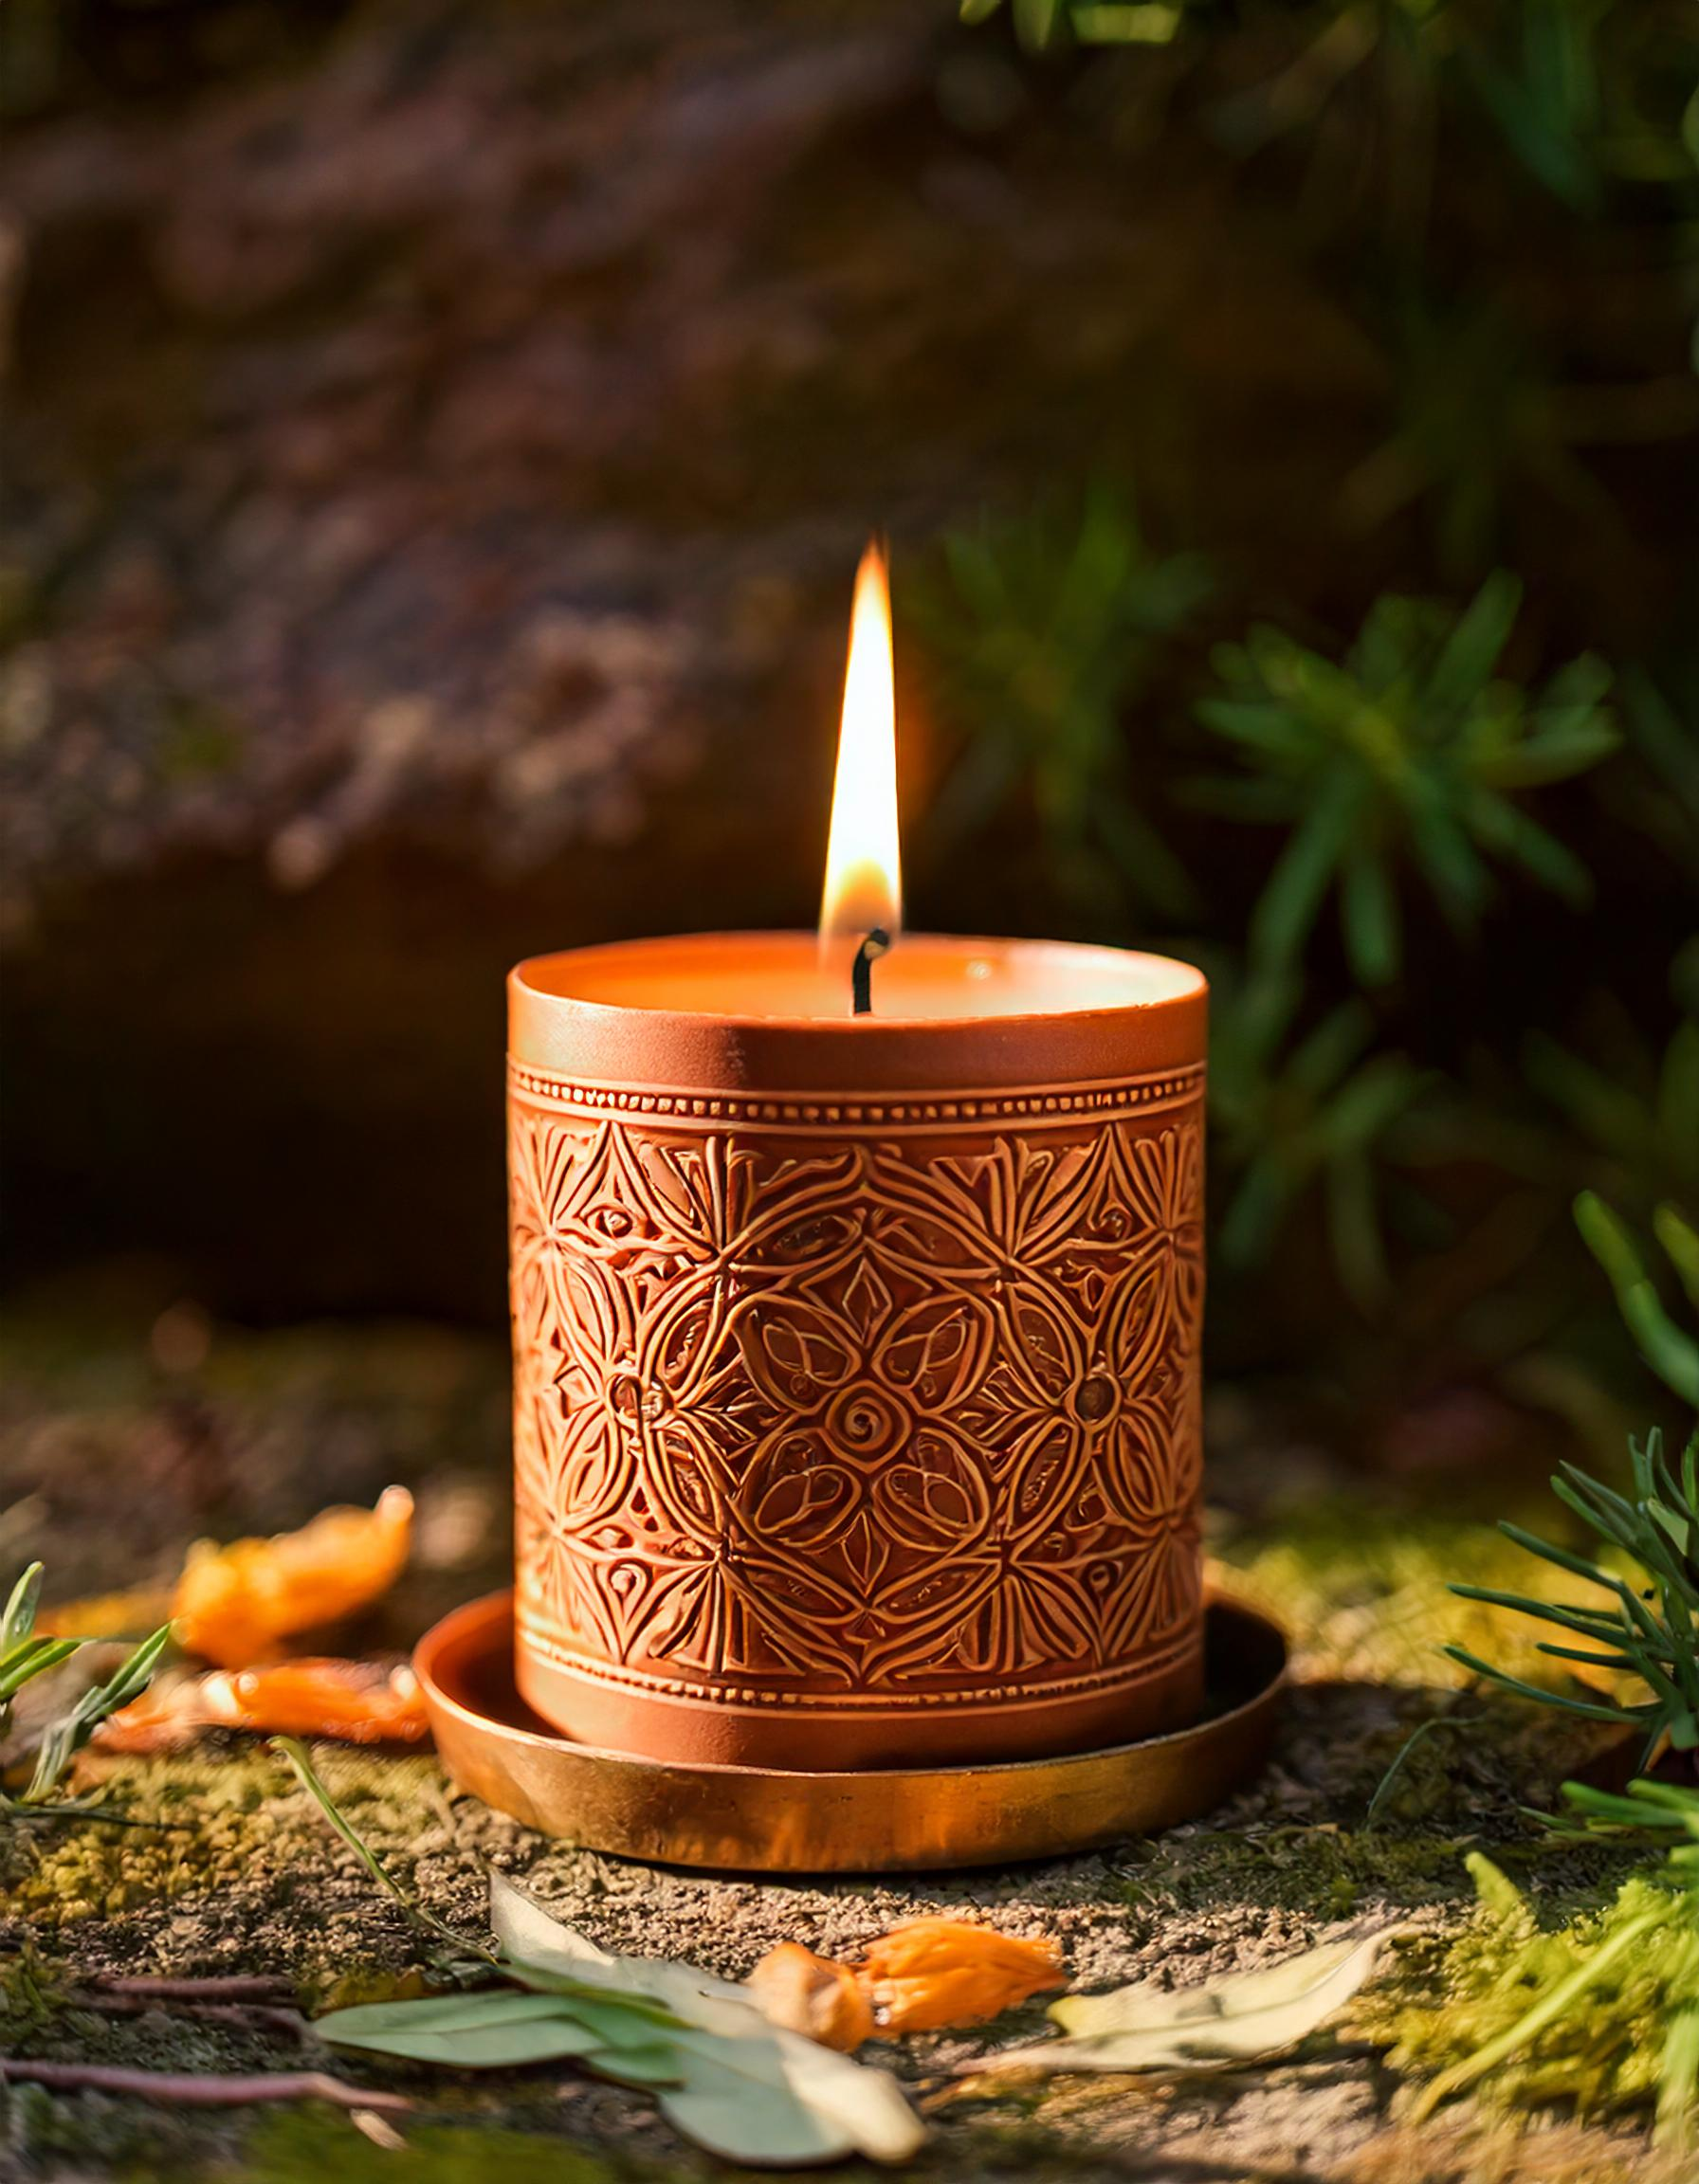
\includegraphics[width=\paperwidth,height=\paperheight]{bougie_style_cover_HD}%
}
\centering
\vspace*{3cm}
\par\normalfont\fontsize{35}{35}\sffamily\selectfont
\textbf{\textcolor{white}{Guide des Bougies Marocaines}}\\
\noindent{\LARGE \fcolorbox{white}{green!30!}{\textcolor{black}{Artisanat durable}}}\par

\vspace*{1cm}
{\Huge \fcolorbox{black}{white}{Créer, Vendre et Valoriser} }\par
\vspace*{5cm} % Réduit de 14cm à 5cm
{\huge \fcolorbox{black}{white}{\textbf{\textsc{Lumiere Academy}}} }
% Nom de l'éditeur
\endgroup
\newpage
%----------------------------------------------------------------------------------------
%	COPYRIGHT PAGE
%----------------------------------------------------------------------------------------
\afterpage{\null\newpage}

~\vfill
\noindent
\textcopyright\ Lumière Academy, 2024. Tous droits réservés.\par
\noindent
Ce document est la propriété de Lumière Academy. Aucune reproduction, totale ou partielle, n'est autorisée sans consentement écrit préalable.\par
\noindent
Pour toute demande \\ \url{https://lumiereacademy.com/contact}.\par

%----------------------------------------------------------------------------------------
%	TABLE OF CONTENTS
%----------------------------------------------------------------------------------------
\chapterimage{images/headers/cover-1.jpg} % heading image

\pagestyle{empty} % No headers

\renewcommand\contentsname{Table des matières}
\renewcommand{\bibname}{Bibliographie}
\tableofcontents% Print the table of contents itself

%\cleardoublepage % Forces the first chapter to start on an odd page so it's on the right

\pagestyle{fancy} % Print headers again


\chapterimage{images/headers/cover-1.jpg} % heading image
\onecolumn

\newpage
\part*{Préface}

\vspace{0.5cm}

\noindent Ma passion pour les produits artisanaux est née d’une prise de conscience écologique. En cherchant à réduire ma consommation de produits chimiques, j’ai commencé à fabriquer mes propres cosmétiques maison. Chaque création représentait un pas vers un mode de vie plus respble. Puis, en voyant toutes ces cires inutilisées issues de mes baumes et crèmes, une question m’est venue comment les réutiliser ? C’est ainsi que j’ai fabriqué ma première bougie. Ce fut une révélation je pouvais créer quelque chose de beau, utile, et écologique, tout en explorant ma créativité.

\vspace{0.5cm}

\noindent Ce livre est bien plus qu’un simple guide technique. Il est une invitation à explorer un univers où la cire se transforme en art, où les parfums éveillent les sens, et où les bougies deviennent des messagères d’émotions. Que vous soyez un amateur désireux de découvrir une nouvelle activité ou un entrepreneur en quête de nouvelles idées, ce livre a été conçu pour vous accompagner à chaque étape.

\vspace{0.5cm}

\noindent En tant que Marocaine, je suis profondément inspirée par la richesse de notre culture et de notre artisanat. À travers ce guide, je partage non seulement les secrets de la fabrication de bougies, mais aussi des anecdotes et des techniques adaptées à notre contexte local. Par exemple, avez-vous déjà pensé à utiliser des huiles essentielles issues de nos ressources naturelles, comme l’argan ou le romarin, pour parfumer vos créations ? Ces trésors marocains ajoutent une touche unique et authentique à vos bougies.

\vspace{0.5cm}

\noindent Mon parcours, enraciné dans les sciences naturelles et la gestion de projets, m’a permis de combiner expertise scientifique et passion artisanale. Forte d’une formation en biodiversité et conservation, j’intègre dans chaque création une approche respectueuse de l’environnement. Cet aspect, plus que jamais crucial dans notre monde d’aujourd’hui, est au cœur de mes valeurs et de mon travail.

\vspace{0.5cm}

\noindent Ce livre n’est pas une fin en soi, mais un début. À chaque page, vous trouverez des conseils pratiques, des astuces, et des récits pour vous inspirer. J’espère que ce voyage vous apportera autant de joie qu’il m’en a apporté, et qu’ensemble, nous pourrons illuminer vos maisons et celles de vos proches.

\vspace{1cm}

\noindent Bienvenue dans cet univers lumineux. Prenez vos outils, votre imagination, et laissez la magie opérer !

\vspace{1.5cm}

\hfill Souheila JEBBARI \\
\hfill Novembre 2024

\part{Introduction}


\chapter{Pourquoi fabriquer vos bougies ?}

\section{Introduction}


\begin{definition} La fabrication de bougies est bien plus qu’une simple activité manuelle. Elle représente une passerelle vers un univers riche d’exploration artistique, de pratiques respectueuses de l’environnement, et d’une profonde connexion avec des traditions ancrées dans l’histoire et la culture. Que vous soyez passionné d’artisanat ou en quête d’une activité créative, ce chapitre pose les bases pour comprendre et apprécier cet art lumineux. \end{definition}

\begin{itemize} \item \textbf{L’histoire et le symbolisme des bougies} Découvrez leur rôle spirituel, artistique, et culturel, tant au Maroc qu’à travers le monde, et comprenez pourquoi elles continuent de fasciner. \item \textbf{Les avantages de la fabrication artisanale} Plongez dans un art qui allie créativité, durabilité, et opportunités économiques, tout en explorant des matériaux comme la cire de soja ou d’abeille. \item \textbf{Des témoignages inspirants} Rencontrez des artisans marocains qui ont su marier traditions locales et techniques modernes pour transformer leur passion en succès. \item \textbf{Les premières étapes pratiques} Familiarisez-vous avec les matériaux essentiels (cires, mèches, parfums) et apprenez à organiser un espace de travail fonctionnel et sécurisé. \end{itemize}

\noindent Ce chapitre vous accompagnera dans une découverte où les bougies se révèlent comme des œuvres d’art, des objets porteurs de traditions, et des créations empreintes d’émotions. Vous serez également introduit aux bases techniques qui permettront de transformer vos idées en réalisations concrètes.

\begin{remark} La fabrication de bougies, bien qu’intemporelle dans son symbolisme, est aussi un art moderne qui peut enrichir votre quotidien. Plongeons ensemble dans le symbolisme fascinant et les bénéfices pratiques qui font de cet art une activité incontournable. \end{remark}

\section{Le Symbolisme des Bougies Une Passion Universelle}

\begin{definition} Les bougies sont bien plus que de simples objets utilitaires. Elles traversent les âges comme des témoins silencieux de l’histoire humaine, éclairant nos nuits, marquant des rituels sacrés et enveloppant nos instants de recueillement d’une lumière douce et apaisante. \end{definition}

\begin{remark} Au Maroc, les bougies occupent une place unique, mêlant spiritualité, tradition et art. Lors de ma visite à un souk de Marrakech, j’ai été frappée par la beauté des bougies artisanales ornées de motifs dorés. Elles semblaient capturer l’âme de notre culture, entre lumière divine et chaleur humaine. \end{remark}

\begin{remark} Le symbolisme des bougies nous rappelle leur importance culturelle et émotionnelle. Elles incarnent des valeurs universelles de paix, d’espoir et de célébration, tout en reflétant les identités culturelles locales à travers des motifs, des formes et des parfums uniques. Mais qu’en est-il des avantages pratiques et personnels que procure leur fabrication ? Découvrons ensemble les multiples facettes de cet art créatif. \end{remark}

\begin{figure}[htbp]
    \centering
    \includegraphics[
        width=0.6\textwidth,    % 60% de la largeur du texte
        height=0.4\textheight,  % 40% de la hauteur du texte
        keepaspectratio         % Maintient le ratio d'aspect pour éviter la déformation
    ]{images/chapitre1/image-ramadan.jpg}
    \caption{Lanterne ornementale avec bougie allumée}
    \label{fig:image_lanterne}
\end{figure}


\subsection*{Une Lumière dans Nos Traditions}

Les bougies sont profondément enracinées dans les traditions marocaines, symbolisant bien plus que la simple lumière. Voici quelques exemples qui témoignent de leur importance

\begin{itemize} \item \textbf{Cérémonies religieuses} Lors de fêtes comme Achoura, des bougies illuminent les foyers, symbolisant la guidance et la lumière divine qui éclaire le chemin des croyants. Leur douce lueur invite à la réflexion et au partage. \item \textbf{Décorations festives} Dans les mariages traditionnels marocains, les bougies ornées de motifs dorés ou argentés embellissent les plateaux portés par les mariées, ajoutant une touche de majesté et de solennité. Ces bougies incarnent également les vœux de bonheur et de prospérité pour les jeunes mariés. \item \textbf{Ambiances parfumées} Les bougies parfumées aux huiles essentielles locales, comme le romarin, la lavande ou l’argan, apportent une atmosphère de sérénité dans les foyers. Leur parfum évoque les montagnes de l’Atlas, les champs de lavande du Rif ou encore les vergers de fleurs d’oranger. \item \textbf{Symboles de paix et d’espoir} Dans les moments difficiles, allumer une bougie devient un geste de solidarité et d’espoir pour des jours meilleurs, une tradition universelle empreinte de sagesse et de résilience. Elle incarne également une mémoire vivante, souvent allumée en hommage aux êtres chers disparus. \end{itemize}

\begin{remark} Ces traditions, riches en symbolisme et en significations, se marient aujourd'hui avec des techniques modernes pour créer des bougies uniques et personnelles. L’alliance de l’histoire et de l’innovation fait de chaque bougie un objet qui raconte une histoire propre, tout en respectant les héritages du passé. \end{remark}

\subsection*{Une Source d’Émotion et de Mémoire}

\begin{corollary} Chaque bougie allumée est une manifestation de lumière et de chaleur humaine. Dans une maison marocaine, une bougie n’est pas seulement un objet c’est un vecteur d’émotions, une porte vers des souvenirs précieux et un reflet de notre attachement à nos racines. Allumer une bougie, c’est raviver un souvenir ou honorer une émotion. \end{corollary}

\begin{figure}[htbp]
    \centering
    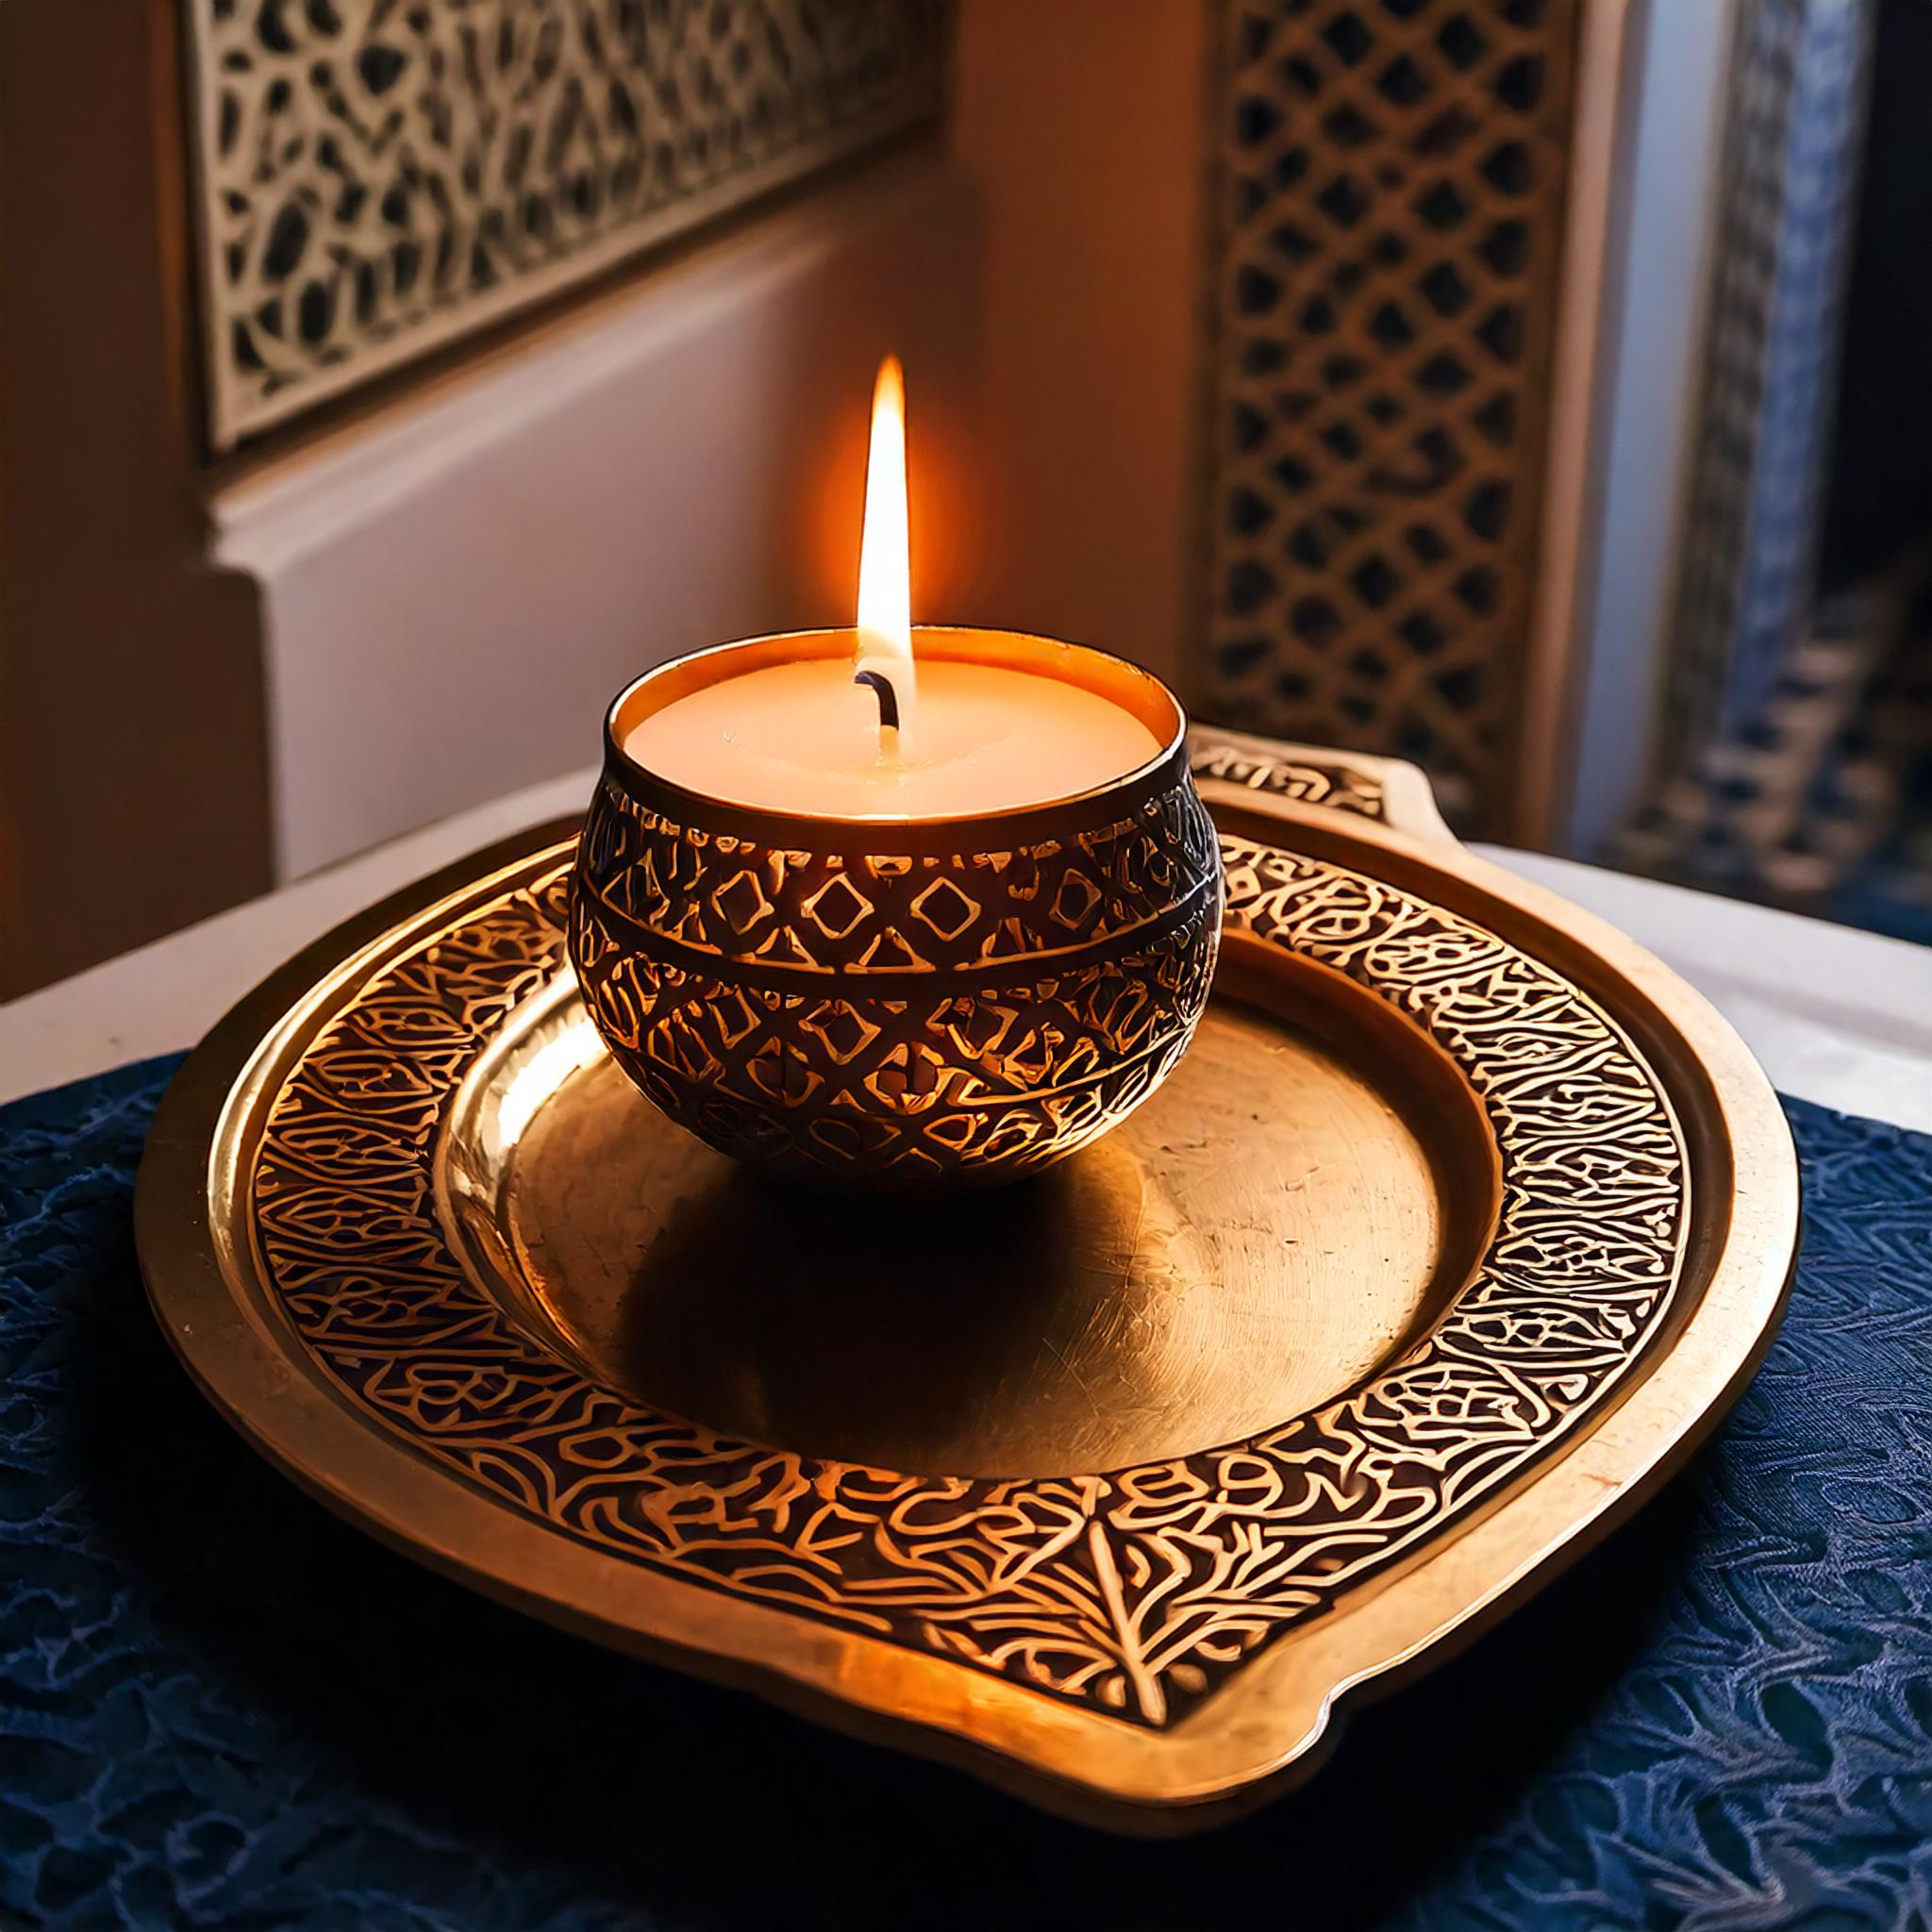
\includegraphics[
        width=0.6\textwidth,    % 60% de la largeur du texte
        height=0.4\textheight,  % 40% de la hauteur du texte
        keepaspectratio         % Maintient le ratio d'aspect pour éviter la déformation
    ]{images/chapitre1/nostalgie-bougie.jpg}
    \caption{Entre Tradition et Émotion}
    \label{fig:image_bougie_tradition_emotion}
\end{figure}


\begin{example} Lors d’un atelier organisé à Essaouira, une artisane racontait « Une bougie n’est pas simplement une source de lumière, c’est une mémoire. Elle porte en elle des histoires, des lieux et des moments qui nous unissent à nos racines et à nos aspirations. » \end{example}

\begin{remark} Le symbolisme des bougies nous rappelle leur importance culturelle, émotionnelle et spirituelle. En les façonnant de vos propres mains, vous créez non seulement un objet, mais aussi une œuvre qui incarne des souvenirs et des émotions. Dans la section suivante, explorons les avantages personnels et pratiques que procure la fabrication artisanale de bougies. \end{remark}

\section{Les Avantages de la Fabrication Artisanale}

\begin{definition}
Fabriquer ses propres bougies, c’est bien plus que créer un objet lumineux. C’est une aventure qui marie créativité, engagement écologique et opportunités économiques. Cette activité, simple en apparence, peut illuminer bien des aspects de votre vie.
\end{definition}

\subsection*{Expression Artistique}

\begin{remark}
Chaque bougie est une toile vierge, une opportunité d’exprimer votre créativité. Ali, un artisan de Fès, sculpte des bougies inspirées des motifs andalous, mêlant harmonieusement tradition et innovation. « Une bougie bien façonnée est comme une œuvre d’art elle capte la lumière et l’âme », aime-t-il dire.
\end{remark}

\begin{figure}[htbp]
    \centering
    \includegraphics[
        width=0.6\textwidth,    % 60% de la largeur du texte
        height=0.4\textheight,  % 40% de la hauteur du texte
        keepaspectratio         % Maintient le ratio d'aspect pour éviter la déformation
    ]{images/chapitre1/bougie-artistique.jpg}
    \caption{Atelier de bougies décorées. Fabrication artistique de bougies}
    \label{fig:image_bougie_art}
\end{figure}


Jouer avec les couleurs, les textures et les parfums permet de transformer une simple cire en une création unique. Par exemple, les parfums locaux comme la fleur d’oranger ou la menthe marocaine peuvent insuffler une touche authentique à vos bougies, rappelant les senteurs des marchés et des paysages marocains.

\begin{remark}
La maîtrise des matériaux comme la cire de soja, idéale pour une diffusion optimale des parfums, ou la cire d’abeille, prisée pour sa combustion lente et son parfum naturel, ouvre des possibilités infinies. Associée à des techniques modernes telles que le marbrage, le moulage complexe ou l’ajout de couches superposées, elle permet de créer des designs aussi élégants qu’originaux.
\end{remark}

En expérimentant avec des techniques avancées, telles que
\begin{itemize}
    \item \textbf{Le marbrage} joue sur les effets de texture et de mouvement des couleurs pour un rendu artistique.
    \item \textbf{Les motifs en relief} inspirés des zelliges marocains.
    \item \textbf{La combinaison de matériaux naturels} comme des mèches en bois et des huiles essentielles locales.
\end{itemize}
vous pouvez allier innovation et respect des traditions.

Les cires elles-mêmes deviennent un support d’expression. Tandis que la \textbf{cire de coco} permet des finitions douces et soyeuses, la \textbf{cire de soja} est plébiscitée pour ses possibilités de teintes vibrantes et sa facilité à capturer des parfums complexes. Quant à la \textbf{cire d’abeille}, elle confère une dimension écologique et luxueuse, idéale pour des créations haut de gamme.

\subsection*{Engagement Écologique Allier Tradition et Durabilité}

\begin{corollary}
En choisissant des matériaux respectueux de l’environnement, la fabrication artisanale de bougies peut contribuer activement à la préservation de la planète tout en valorisant les richesses locales. Contrairement aux bougies industrielles à base de paraffine, issues de la pétrochimie et générant des émissions de suie, les cires naturelles et les pratiques durables offrent une alternative écologique et esthétique.
\end{corollary}

\subsubsection*{Cires Naturelles Une Alternative Écologique}

Opter pour des cires naturelles comme la cire d’abeille ou la cire de soja présente des avantages écologiques significatifs 
\begin{figure}[htbp]
    \centering
    \includegraphics[
        width=0.6\textwidth,    % 60% de la largeur du texte
        height=0.4\textheight,  % 40% de la hauteur du texte
        keepaspectratio         % Maintient le ratio d'aspect pour éviter la déformation
    ]{images/chapitre1/bougie-cire-abeille.jpg}
    \caption{Une bougie faite à la main en cire naturelle avec une texture d'abeilles en nid d'abeille}
    \label{fig:image_bougie_cire_abeille}
\end{figure}



\begin{itemize}
    \item \textbf{Cire d’abeille} Ce produit renouvelable offre une combustion propre, dégage un parfum naturellement doux et apporte une texture luxueuse aux bougies. En valorisant les pratiques apicoles durables, les artisans marocains soutiennent la biodiversité tout en réduisant leur empreinte écologique.
    \item \textbf{Cire de soja} Issue de l’huile de soja, cette cire végétale est biodégradable, renouvelable et garantit une combustion lente et propre, tout en diffusant efficacement les parfums. Cependant, il est essentiel de s’assurer que le soja provient de cultures responsables pour éviter les impacts négatifs comme la déforestation.
    \item \textbf{Cire de coco} Plus récente sur le marché, elle est issue de l’huile de noix de coco et se distingue par sa douceur et son excellente diffusion des parfums. Bien que son coût soit plus élevé, elle constitue une option biodégradable et renouvelable.
\end{itemize}

\subsubsection*{Valorisation des Ressources Locales au Maroc}

L’utilisation des ressources naturelles locales est une démarche clé pour minimiser l’empreinte carbone tout en soutenant les économies locales.
\begin{figure}[htbp]
    \centering
    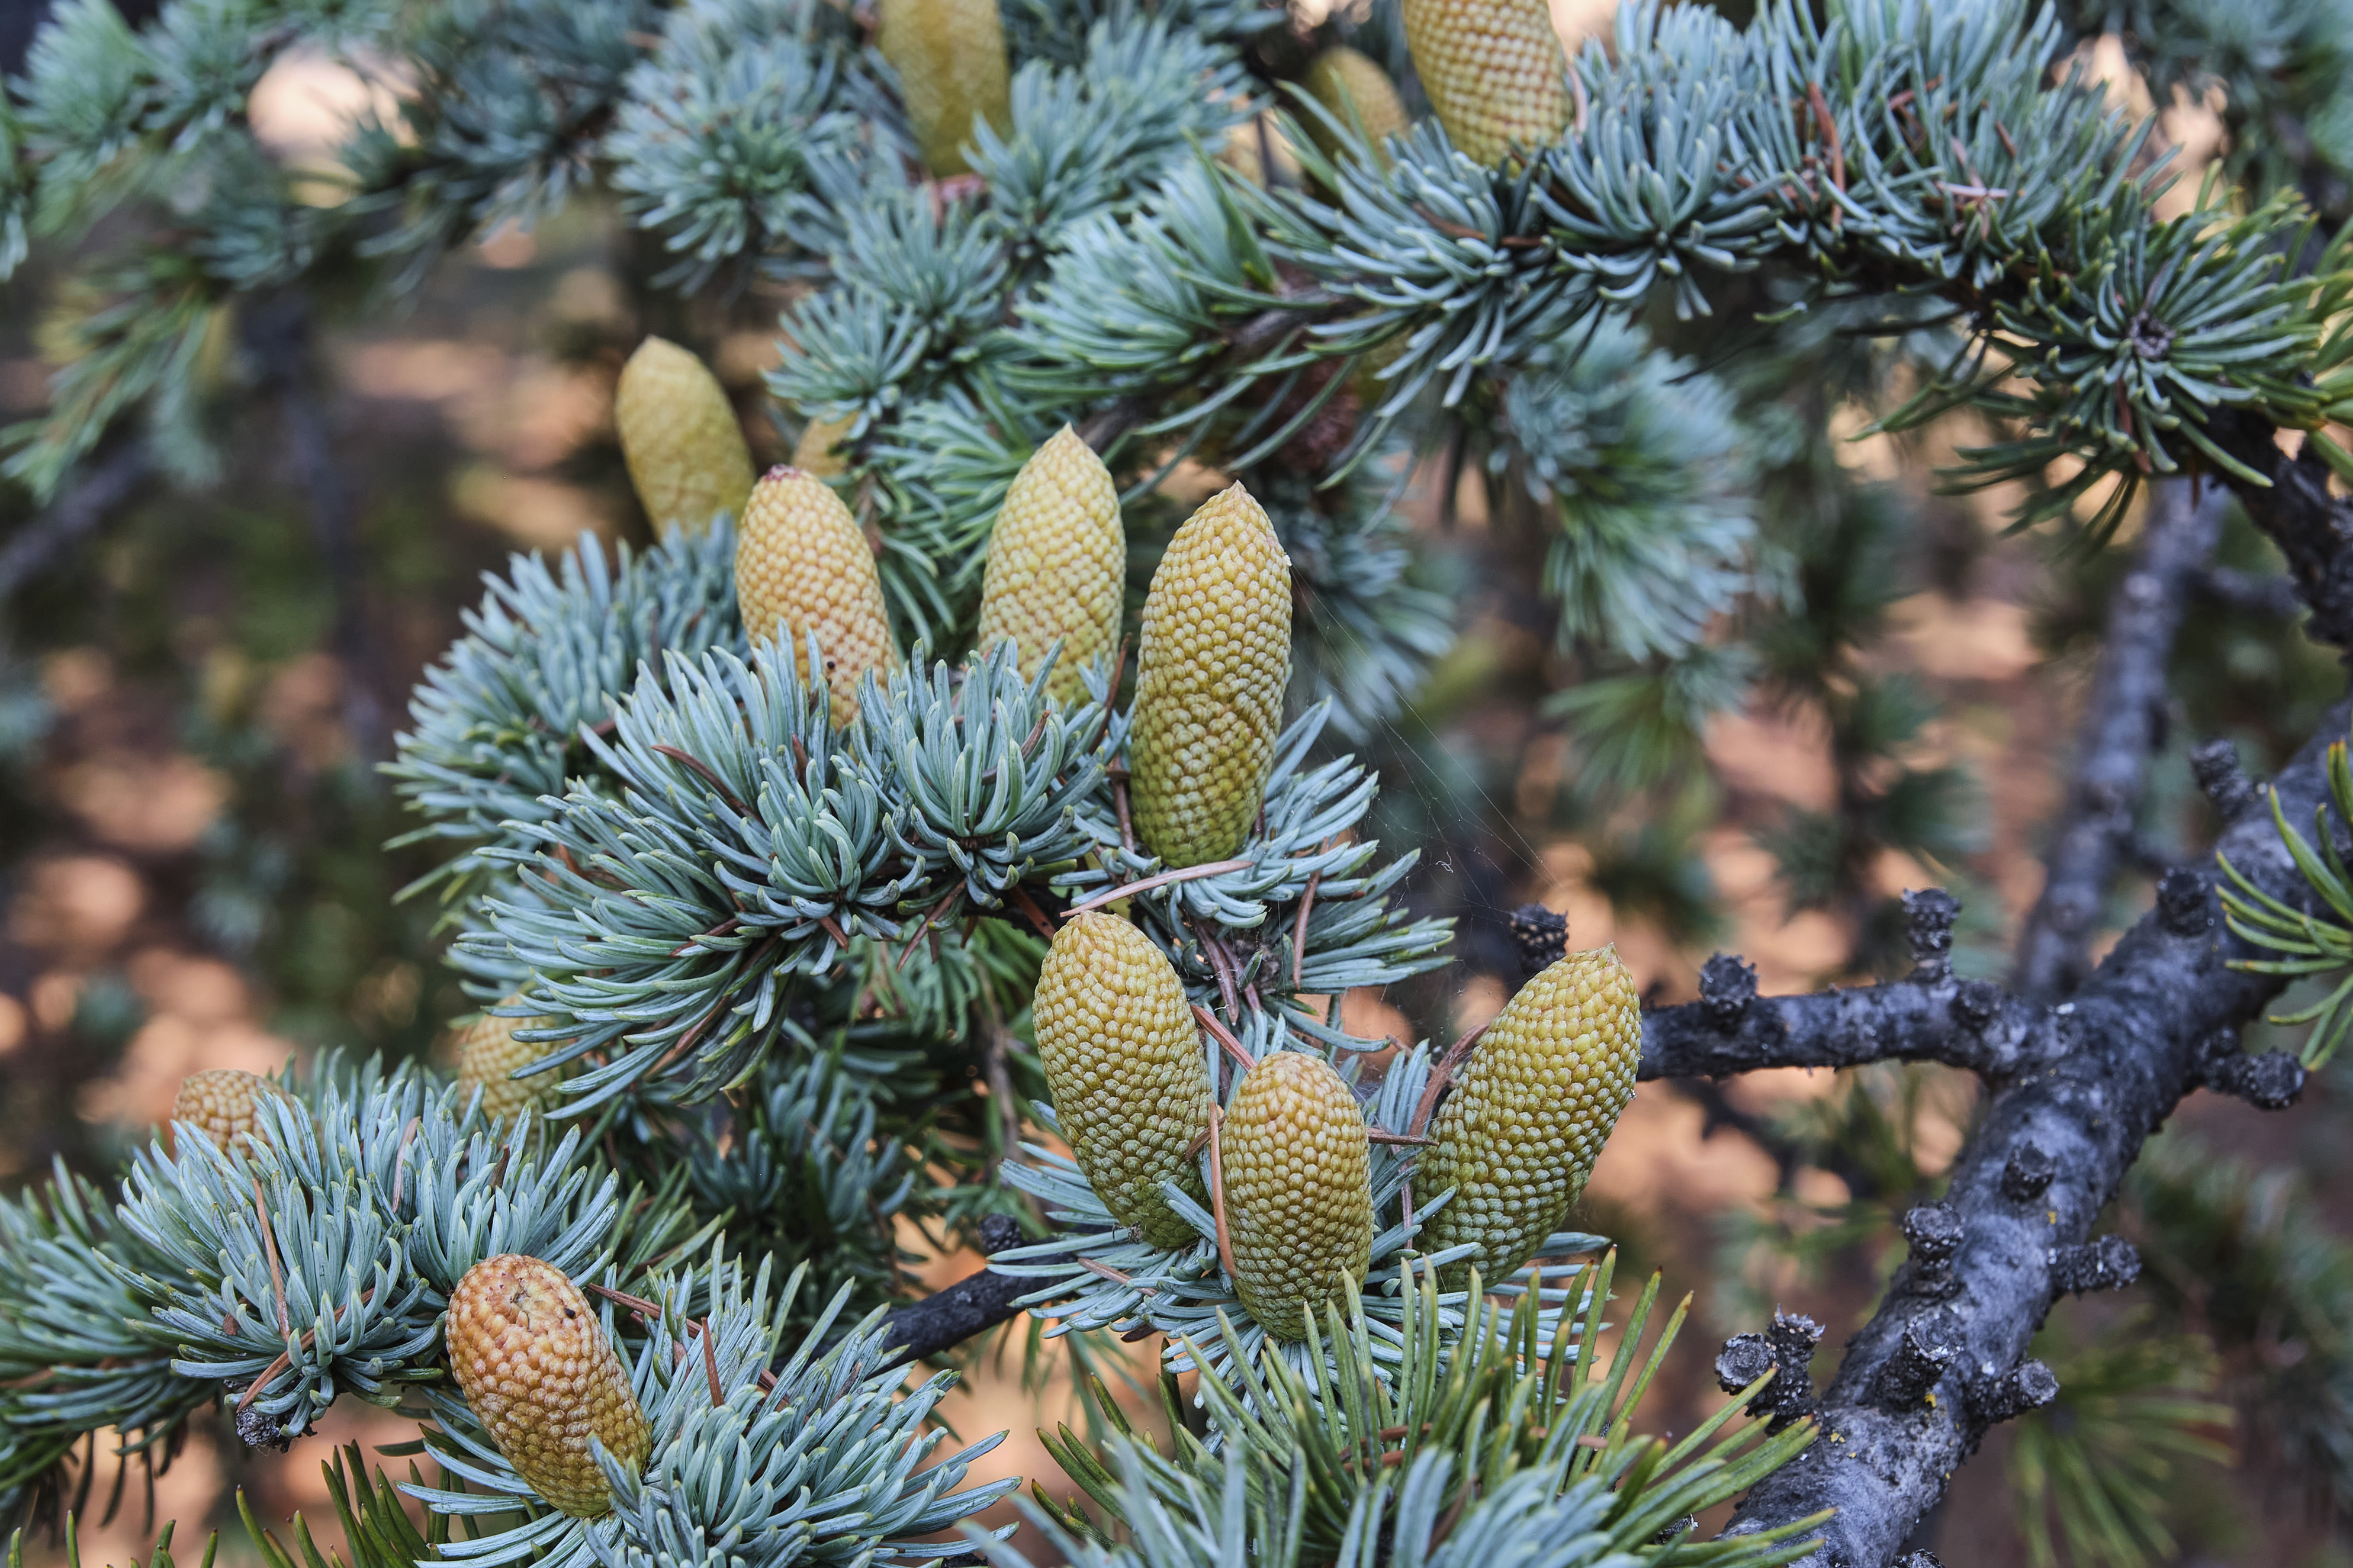
\includegraphics[
        width=0.6\textwidth,    % 60% de la largeur du texte
        height=0.4\textheight,  % 40% de la hauteur du texte
        keepaspectratio         % Maintient le ratio d'aspect pour éviter la déformation
    ]{images/chapitre1/cedre-atlas.jpg}
    \caption{Branche de cèdre de l'Atlas à cônes. Cedrus atlantica}
    \label{fig:cedrus_atlantica}
\end{figure}


\begin{itemize}
    \item \textbf{Huile essentielle de cèdre de l’Atlas} Produite au Maroc, cette huile précieuse est prisée pour ses arômes boisés et ses propriétés thérapeutiques. Elle apporte une touche authentique et locale aux bougies artisanales.
    \item \textbf{Huile essentielle d’eucalyptus} Cultivée au Maroc, elle offre des notes rafraîchissantes et antiseptiques, idéales pour des bougies bien-être.
    \item \textbf{Plantes locales} Intégrer des herbes séchées comme le romarin ou la lavande, cultivées dans les montagnes marocaines, enrichit les bougies d’une dimension visuelle et aromatique unique.
\end{itemize}

\subsubsection*{Autres Pratiques Durables}

Outre le choix des cires et des huiles essentielles, plusieurs pratiques renforcent l’engagement écologique des bougies artisanales.

\begin{figure}[htbp]
    \centering
    \includegraphics[
        width=0.6\textwidth,    % 60% de la largeur du texte
        height=0.4\textheight,  % 40% de la hauteur du texte
        keepaspectratio         % Maintient le ratio d'aspect pour éviter la déformation
    ]{images/chapitre1/meche-bois.jpg}
    \caption{Bocaux en verre vides avec mèches en bois}
    \label{fig:cedrus_atlantica}
\end{figure}

\begin{itemize}
    \item \textbf{Mèches écologiques} Privilégier des mèches en coton non traité ou en bois certifié FSC (provenant de forêts gérées durablement) réduit les impacts environnementaux.
    \item \textbf{Emballages biodégradables} Utiliser des emballages recyclables ou compostables, tels que le papier kraft ou le carton recyclé, évite la pollution plastique.
    \item \textbf{Optimisation de la production} Réduire les déchets de cire en recyclant les résidus dans de nouvelles créations contribue à limiter le gaspillage.
\end{itemize}

\begin{remark}
En adoptant ces pratiques, les artisans marocains peuvent non seulement préserver leur environnement, mais également répondre à une demande croissante pour des produits durables et éthiques. Ainsi, chaque bougie devient non seulement une source de lumière, mais aussi un témoignage d’harmonie entre créativité et respect de la nature.
\end{remark}


\subsection*{Opportunités Économiques L'Artisanat Marocain à la Conquête du Monde}

\begin{remark}
La fabrication artisanale de bougies n'est pas seulement un art, c'est aussi une porte ouverte vers des opportunités économiques infinies. Avec des plateformes en ligne, des événements locaux et des initiatives telles que celles de Lumière Academy, les artisans marocains disposent aujourd'hui de multiples vitrines pour dévoiler leur créativité au-delà des frontières.
\end{remark}

\subsubsection*{Plateformes en Ligne Une Vitrine Internationale}

Grâce à des sites comme Etsy, les artisans marocains peuvent présenter leurs créations à une clientèle mondiale avide d'authenticité. En naviguant sur ces plateformes, on découvre des bougies artisanales marocaines qui racontent des histoires, avec des motifs inspirés des zelliges ou des parfums évoquant les montagnes de l’Atlas.

\begin{example}
Prenons l’exemple de Fatima, une créatrice de Marrakech, qui a récemment lancé sa boutique en ligne. « Lorsque j’ai reçu ma première commande d’Australie, j’ai ressenti une immense fierté, comme si un morceau de ma culture voyageait dans le monde », raconte-t-elle.
\end{example}

Ces plateformes ne sont pas seulement des marchés, mais aussi des outils permettant aux artisans de partager leur passion, leur savoir-faire et leur identité culturelle avec un public diversifié.

\subsubsection*{Événements Locaux Le Savoir-Faire au Cœur des Communautés}

Les foires et marchés artisanaux, notamment ceux de Marrakech ou Essaouira, sont des rendez-vous incontournables pour les artisans. Ces événements attirent aussi bien les habitants que les touristes, créant un espace où tradition et modernité se rencontrent.

\begin{example}
Lors du Festival des Arts de l’Artisanat à Essaouira, les bougies artisanales de Youssef, un jeune entrepreneur, ont attiré des foules. Ses créations, mêlant des parfums locaux comme la fleur d’oranger à des designs modernes, se sont vendues en quelques heures.
\end{example}

Ces événements permettent non seulement de vendre des produits, mais aussi de tisser des liens avec les clients et de renforcer la visibilité des artisans sur le plan local et international.

\subsubsection*{Lumière Academy Allier Savoir-Faire et Transmission}

Lumière Academy, située à Rabat, illustre parfaitement comment l’artisanat peut devenir une force motrice pour l’économie locale tout en valorisant la culture marocaine. Fondée en 2023, cette entreprise familiale propose une expérience unique autour de l’art de la bougie

\begin{itemize}
    \item \textbf{Ateliers créatifs} Lumière Academy organise des sessions immersives où touristes et locaux apprennent à fabriquer leurs propres bougies. Ces ateliers sont non seulement éducatifs mais aussi un moyen de créer des souvenirs personnalisés ancrés dans la culture marocaine.
    \item \textbf{Formations en ligne} En complément de leurs ateliers sur place, Lumière Academy propose des formations accessibles via leur site internet. Ces cours en ligne offrent aux participants, même éloignés, l’opportunité d’apprendre les techniques de fabrication artisanale à leur rythme.
    \item \textbf{Formations en présentiel} Avec des sessions pratiques à Rabat, Lumière Academy partage son savoir-faire avec des passionnés désireux de maîtriser l’art de la bougie tout en s’imprégnant de l’ambiance marocaine.
    \item \textbf{Team-building} Les ateliers de team-building de Lumière Academy offrent une nouvelle approche du travail d'équipe en stimulant la créativité et en renforçant les liens au sein des groupes, dans une atmosphère détendue et inspirante.
    \item \textbf{Magasin} En parallèle, Lumière Academy propose une gamme de bougies artisanales uniques, disponibles dans leur magasin. Chaque création raconte une histoire, inspirée de la culture marocaine et des valeurs de durabilité et d'innovation.
\end{itemize}

\begin{remark}
« À travers Lumière Academy, nous voulons partager la lumière de l’artisanat marocain avec le monde entier, tout en offrant aux participants une expérience inoubliable et immersive », explique l’équipe fondatrice.
\end{remark}

\subsubsection*{Allier Tradition et Modernité Le Succès des Artisans Marocains}

De nombreux artisans marocains savent marier le charme intemporel des traditions avec les attentes contemporaines. Cette combinaison unique est un atout majeur qui séduit une clientèle exigeante.

\begin{example}
À Marrakech, la marque « Côté Bougie » illustre parfaitement cette symbiose. En travaillant avec des artisans locaux, elle crée des collections qui célèbrent les gestes séculaires tout en intégrant un design épuré et moderne. Ces bougies deviennent des œuvres d’art qui ornent les intérieurs à travers le monde.
\end{example}

Aïcha, une artisane de Casablanca, a également su transformer sa passion en une marque florissante. En adoptant un positionnement écologique, elle utilise des cires naturelles et des parfums locaux pour concevoir des bougies élégantes et respectueuses de l’environnement. « Chaque bougie que je vends est comme une étincelle d’espoir, un message de durabilité et de beauté », dit-elle avec émotion.

\subsubsection*{Conclusion Rayonner Ensemble}

Les opportunités économiques dans la fabrication de bougies artisanales montrent qu’il est possible de conjuguer créativité, tradition et modernité pour bâtir une activité prospère. Qu’il s’agisse de toucher un public international via des plateformes en ligne, de captiver les foules lors d’événements locaux, ou encore de transmettre ce savoir-faire unique grâce à des initiatives comme celles de Lumière Academy, l’artisanat marocain a tout pour rayonner.


\subsection*{Développement Personnel Une Alchimie de Bien-Être et de Compétences}

\begin{remark}
La fabrication artisanale de bougies dépasse la simple création d’un objet esthétique. C’est une pratique qui cultive à la fois l’apaisement mental et le développement de compétences clés, enrichissant ainsi la vie personnelle et professionnelle de ceux qui s’y adonnent.
\end{remark}

\subsubsection*{Une Activité Méditative et Thérapeutique}

Dans le silence d’un atelier ou la chaleur d’un espace créatif, la fabrication de bougies offre un moment d’évasion. Le choix des cires, des parfums et des couleurs engage les sens et favorise un état de concentration comparable à la méditation. Chaque étape, du mélange des cires à la création des motifs, devient une danse silencieuse entre les mains et l’esprit.

\begin{figure}[htbp]
    \centering
    \includegraphics[
        width=0.6\textwidth,    % 60% de la largeur du texte
        height=0.4\textheight,  % 40% de la hauteur du texte
        keepaspectratio         % Maintient le ratio d'aspect pour éviter la déformation
    ]{images/chapitre1/meche-bois.jpg}
    \caption{Bocaux en verre vides avec mèches en bois}
    \label{fig:cedrus_atlantica}
\end{figure}

\begin{example}
Amina, une participante à un atelier organisé par Lumière Academy, raconte « Chaque bougie que je crée est comme une histoire. Les parfums me rappellent des souvenirs, les couleurs apaisent mon esprit, et le processus me reconnecte avec moi-même. »
\end{example}

Certaines créations, comme les bougies de lithothérapie, vont encore plus loin en combinant les bienfaits apaisants des bougies à ceux des pierres semi-précieuses, transformant chaque flamme en un guide vers l’épanouissement personnel.

\subsubsection*{Développement de Compétences en Gestion de Projet}

La fabrication de bougies n’est pas qu’un exercice de détente ; c’est aussi un art exigeant qui requiert organisation et rigueur. De la conception à la commercialisation, chaque projet de bougie artisanale implique une série d’étapes interconnectées qui renforcent des compétences essentielles

\begin{itemize}
    \item \textbf{Planification} Définir un calendrier précis, organiser les étapes de production et anticiper les besoins en matériaux.
    \item \textbf{Organisation} Gérer efficacement les ressources, qu’elles soient matérielles ou humaines, et synchroniser les différentes phases du projet.
    \item \textbf{Créativité} Imaginer des designs uniques et audacieux, associer des couleurs harmonieuses et choisir des parfums évocateurs.
    \item \textbf{Marketing} Élaborer une identité de marque captivante, développer une stratégie de promotion efficace et séduire une clientèle diversifiée.
\end{itemize}

\begin{remark}
Chez Lumière Academy, nous avons constaté que chaque formation ou atelier en fabrication de bougies est une opportunité pour les participants de découvrir leurs capacités organisationnelles et leur créativité innée. Nos programmes, y compris nos formations en ligne, permettent à chacun d’acquérir et de perfectionner ces compétences dans un cadre à la fois ludique et professionnel.
\end{remark}

\subsubsection*{Un Engagement pour l’Insertion Professionnelle et Sociale}

Lumière Academy est fière de collaborer avec l’Association Marocaine d’Appui à la Promotion de la Petite Entreprise (AMAPPE), une organisation reconnue pour son rôle dans l’accompagnement des populations vulnérables au Maroc. Ensemble, nous travaillons à promouvoir la réinsertion professionnelle de populations telles que les femmes, les jeunes et les réfugiés, en leur offrant des formations pratiques dans la fabrication de bougies.

\begin{example}
Dans le cadre de ce partenariat, des ateliers de fabrication de bougies ont été organisés pour des groupes accompagnés par l’AMAPPE, comme les participants au Programme d’Insertion Socio-Économique des Réfugiés Urbains au Maroc (PISERUMA). Ces sessions permettent aux participants d’acquérir des compétences artisanales tout en les préparant à créer leurs propres micro-entreprises.
\end{example}

En s’appuyant sur des valeurs de durabilité et de solidarité, Lumière Academy contribue activement à la lutte contre le chômage et à l’autonomisation des populations défavorisées. Ces initiatives incarnent notre vision d’un artisanat inclusif, qui allie savoir-faire local et impact social.

\subsubsection*{Un Tremplin pour la Croissance Personnelle et Professionnelle}

Ce qui commence comme un simple passe-temps peut évoluer en une véritable aventure de développement personnel. Les participants aux ateliers ou aux formations rapportent souvent un sentiment d’accomplissement en voyant leurs créations prendre forme. De plus, pour ceux qui souhaitent aller plus loin, cette activité peut servir de tremplin pour bâtir un projet entrepreneurial solide.

\begin{example}
Lors d’une formation intensive à Lumière Academy, Youssef, un entrepreneur débutant, a appris à gérer les étapes de fabrication de bougies et à développer une marque écoresponsable. Aujourd’hui, il exporte ses créations parfumées aux huiles essentielles marocaines vers l’Europe, tout en valorisant les ressources locales.
\end{example}

\subsubsection*{Conclusion L'Art de Se Réinventer}

La fabrication artisanale de bougies est une alchimie subtile entre relaxation, expression artistique et apprentissage pratique. Elle invite à s’épanouir, à découvrir des talents insoupçonnés et à transformer un instant de détente en une compétence précieuse. Chez Lumière Academy, nous sommes fiers d’accompagner nos participants dans ce voyage lumineux et inspirant.

\begin{remark}
« Créer une bougie, c’est allumer une flamme en soi », résume Salma, une formatrice passionnée de Lumière Academy. « Que ce soit pour le plaisir ou pour bâtir une entreprise, chaque bougie reflète un morceau de votre histoire et de votre potentiel. »
\end{remark}

\subsection*{Personnalisation et Unicité Une Alchimie entre Culture et Créativité}

Créer vos propres bougies offre une liberté inégalée pour exprimer votre créativité et proposer des produits sur mesure. Ces créations deviennent autant d’objets uniques, où se mêlent inspirations culturelles, savoir-faire artisanal et préférences personnelles.

\subsubsection*{L’Art du Zellige dans la Conception de Bougies}

Le \textit{zellige}, art ancestral marocain des mosaïques en terre cuite émaillée, inspire profondément la création de bougies artisanales. Ce savoir-faire, reconnu pour ses motifs géométriques complexes et ses palettes de couleurs vibrantes, peut être intégré de plusieurs façons dans le design des bougies

\begin{itemize}
    \item \textbf{Décoration des contenants} Utiliser des pots ou des verres ornés de motifs de \textit{zellige} pour contenir les bougies. Ces objets deviennent alors de véritables pièces décoratives, sublimant chaque intérieur. Par exemple, des artisans comme Salima Filali réinterprètent les motifs traditionnels pour créer des contenants élégants et sophistiqués.
    \item \textbf{Incorporation dans la cire} Reproduire des reliefs ou des impressions de motifs de \textit{zellige} directement sur la surface des bougies. Ces détails artistiques transforment chaque pièce en une œuvre d’art unique, hommage à l’esthétique marocaine.
\end{itemize}

\begin{example}
Lors d’un atelier organisé par Lumière Academy, les participants ont appris à créer des bougies inspirées du \textit{zellige}. Les résultats étaient impressionnants des motifs délicats imprimés dans la cire et des contenants peints à la main, chacun racontant une histoire unique.
\end{example}

\subsubsection*{Des Parfums qui Rendent Hommage au Maroc}

La personnalisation s’étend aussi aux choix de parfums, permettant de capturer l’essence même du Maroc dans chaque création. Les fragrances emblématiques comme le jasmin et l’ambre évoquent des paysages, des marchés et des moments intimes chargés de souvenirs.

\begin{itemize}
    \item \textbf{Jasmin} Avec son arôme floral envoûtant, le jasmin incarne douceur et sérénité. Il est souvent utilisé pour créer une ambiance apaisante et romantique.
    \item \textbf{Ambre} Ses notes chaudes et résineuses apportent profondeur et sensualité, évoquant les parfums des souks marocains.
\end{itemize}

\begin{remark}
La combinaison du jasmin et de l’ambre crée une expérience olfactive à la fois exotique et chaleureuse, transportant les utilisateurs au cœur des jardins marocains ou des ruelles animées de Marrakech.
\end{remark}

\subsubsection*{Les Atouts de la Personnalisation}

La création de bougies personnalisées présente de nombreux avantages, tant pour les artisans que pour les utilisateurs

\begin{itemize}
    \item \textbf{Séduction des clients} Proposer des bougies sur mesure répond aux attentes d’une clientèle en quête d’authenticité et d’originalité.
    \item \textbf{Cadeaux mémorables} Offrir une bougie personnalisée, conçue selon les goûts et préférences du destinataire, est un geste attentionné et unique.
    \item \textbf{Expression artistique} Pour les artisans, la personnalisation est une opportunité d’exprimer leur créativité en intégrant des éléments culturels, esthétiques et émotionnels dans chaque pièce.
\end{itemize}

\begin{example}
Chez Lumière Academy, nous encourageons nos participants à repousser les limites de leur imagination. Lors d’une formation, un groupe d’apprenants a conçu une collection de bougies inspirées des saisons marocaines, associant des parfums de menthe fraîche au printemps et de bois de cèdre en hiver. Ces créations ont rapidement trouvé leur place sur les étagères de notre boutique.
\end{example}

\subsubsection*{Une Fusion entre Patrimoine et Innovation}

La personnalisation permet d’ancrer chaque création dans une double dynamique celle de l’héritage culturel marocain et celle de l’innovation contemporaine. En mêlant des techniques artisanales ancestrales, comme l’art du \textit{zellige}, à des parfums évocateurs, chaque bougie devient une invitation à la découverte sensorielle.

\begin{remark}
« La personnalisation, c’est donner une âme à chaque bougie », explique Salma, artisane chez Lumière Academy. « Une bougie n’est pas seulement un objet ; c’est une histoire, un voyage, une émotion. »
\end{remark}

\subsubsection*{Conclusion Un Art Intemporel et Unique}

Créer des bougies personnalisées, c’est bien plus qu’une simple activité manuelle c’est une démarche artistique et émotionnelle. Chaque pièce raconte une histoire et offre une expérience unique, qu’il s’agisse d’un cadeau, d’un objet décoratif ou d’un parfum qui réchauffe l’âme. Avec Lumière Academy, nous invitons chacun à découvrir cet art intemporel et à exprimer son unicité à travers des créations qui inspirent et illuminent.

\subsection*{Conclusion}

\begin{corollary}
La fabrication artisanale de bougies est bien plus qu’un simple loisir. C’est une porte ouverte vers une multitude de possibilités créatives et entrepreneuriales, tout en promouvant des valeurs de durabilité et de respect de l’environnement.
\end{corollary}

\begin{remark}
Maintenant que nous avons exploré les avantages variés de la fabrication artisanale, inspirons-nous des récits d’artisans marocains qui ont su transformer cette passion en véritable succès entrepreneurial.
\end{remark}

\section{Témoignages de Réussite Exemples d’Artisans Marocains}

\begin{definition}
Dans chaque bougie artisanale se cache une histoire unique, un éclat de créativité mêlé aux traditions marocaines. Découvrez ces récits inspirants d’artisans qui ont su transformer leur passion en succès, tout en valorisant le patrimoine local.
\end{definition}

\subsection*{Fatima La Lumière des Spas Haut de Gamme}

\begin{remark}
Fatima, une artisane de Marrakech, incarne parfaitement la rencontre entre tradition et innovation. Spécialisée dans les bougies de massage à base de cire d’abeille et d’huiles essentielles locales, elle a su conquérir le cœur des spas prestigieux, tant au Maroc qu’à l’étranger.
\end{remark}

Tout a commencé lorsqu’elle a remarqué une demande croissante pour des produits naturels dans l’industrie du bien-être. Chaque bougie qu’elle crée est un voyage sensoriel, mêlant la douceur de la cire d’abeille à des parfums envoûtants comme la rose de Damas ou le cèdre de l’Atlas. Ses créations, qui symbolisent luxe et authenticité, sont désormais exportées jusqu’en Europe, où elles séduisent une clientèle en quête de produits écologiques et raffinés.

\begin{example}
Fatima raconte « Lorsque mes bougies sont utilisées dans des spas internationaux, je me dis qu’une part de la culture marocaine illumine des espaces de sérénité à travers le monde. »
\end{example}

\subsection*{Youssef L’Éclat des Jardins Andalous}

\begin{corollary}
À Casablanca, Youssef s’est inspiré de l’héritage architectural des jardins andalous pour lancer une collection de bougies décoratives uniques. Son atelier, niché dans la médina historique, est devenu une adresse incontournable pour les locaux et les touristes.
\end{corollary}

Youssef combine des techniques artisanales ancestrales avec un design moderne. En utilisant des moules en terre cuite et des colorants naturels, il recrée les teintes vibrantes et les motifs géométriques des zelliges marocains. Grâce à une stratégie marketing habile sur les réseaux sociaux, ses bougies ont conquis un public international et sont désormais exposées dans des galeries d’art prestigieuses.

\begin{example}
Lors d’un salon de l’artisanat à Marrakech, ses bougies ont été particulièrement remarquées pour leur capacité à marier héritage et modernité. « Chaque bougie que je fabrique raconte une histoire, un fragment de culture transformé en lumière », dit-il avec fierté.
\end{example}

\subsection*{Aïcha La Gardienne des Traditions Amazighs}

Aïcha, basée à Essaouira, puise son inspiration dans les traditions locales pour ses créations. Elle fabrique des bougies en cire végétale, décorées à la main avec des motifs tribaux Amazighs. « Chaque ligne tracée est un hommage à mes ancêtres et à notre patrimoine », déclare-t-elle avec fierté.

Son engagement écologique et culturel lui a permis de se distinguer dans des salons internationaux, où ses bougies racontent l’histoire d’un Maroc intemporel.

\begin{example}
En 2024, Aïcha a remporté un prix au Salon de l’Artisanat Durable de Rabat pour sa collection « Lumières de l’Atlas », qui mêle des matériaux locaux à des designs inspirés des montagnes marocaines.
\end{example}

\subsection*{Un Héritage Lumineux La Symbiose entre Tradition et Modernité}

Ces témoignages montrent que la fabrication de bougies artisanales est bien plus qu’un métier. C’est une manière de préserver et de réinventer le patrimoine marocain tout en répondant aux exigences d’un marché globalisé. Avec créativité et détermination, ces artisans prouvent qu’il est possible de conjuguer tradition et modernité, local et global.

\begin{exercise}
Réfléchissez aux éléments culturels qui pourraient inspirer vos propres créations. Quelles matières, motifs ou senteurs choisiriez-vous pour raconter une histoire à travers vos bougies ?
\end{exercise}

\begin{remark}
Les récits de Fatima, Youssef et Aïcha témoignent de ce que passion, créativité et engagement peuvent accomplir. Ces exemples inspirants montrent que l’artisanat marocain est un trésor vivant, prêt à illuminer les foyers et les cœurs à travers le monde.
\end{remark}

\section{Préparation Matériaux, outils, et espace de travail}

\begin{definition}
Pour se lancer dans la fabrication de bougies, il est essentiel de s’équiper des bons matériaux et outils. Une préparation minutieuse est le socle d’une création réussie, où chaque élément contribue à l’harmonie finale. Au Maroc, le patrimoine artisanal et les ressources locales enrichissent cette expérience.
\end{definition}

\subsection*{Les Essentiels Cires, Mèches, Parfums et Colorants}

\begin{remark}
Chaque type de cire a ses propres caractéristiques, influençant la texture, la combustion et le parfum de vos bougies. 
\end{remark}

\begin{itemize}
    \item Cire de paraffine Facile à manipuler, elle retient bien les parfums. Idéale pour des créations décoratives.
    \item Cire de soja Biodégradable et naturelle, elle garantit une combustion propre et respecte l’environnement.
    \item Cire d’abeille Réputée pour son parfum doux et sa teinte naturelle, elle est parfaite pour des bougies haut de gamme.
\end{itemize}

Les mèches, souvent négligées, jouent un rôle crucial. Préférez des mèches en coton pour une combustion uniforme ou optez pour des mèches en bois, qui ajoutent une touche élégante avec leur crépitement doux. Côté parfums et colorants, le choix de matières premières de qualité comme les huiles essentielles locales (argan, rose de Damas) et des colorants naturels garantit des créations uniques et respectueuses de l’environnement.

\subsection*{Où se Fournir au Maroc Ressources Locales et Marchés}

\begin{exercise}
Soutenez l’économie locale tout en enrichissant vos créations avec des matériaux authentiques.
\end{exercise}

Le Maroc regorge de ressources pour les amateurs de bougies
\begin{itemize}
    \item Les \textbf{souks traditionnels} (Marrakech, Essaouira) Des cires naturelles, huiles essentielles et mèches artisanales.
    \item Les \textbf{fournisseurs locaux en ligne} \href{https://www.lumiereacademy.com}{Lumière Academy} propose des kits complets pour débutants.
    \item Les \textbf{marchés régionaux} Trouvez des produits uniques comme des parfums inspirés des montagnes de l’Atlas ou des colorants extraits de pigments naturels.
\end{itemize}

En privilégiant les circuits courts, vous apportez une dimension locale et écoresponsable à vos créations.

\subsection*{Aménagement de l’Espace de Travail Astuces Pratiques}

\begin{corollary}
Un espace de travail bien organisé n’est pas seulement pratique, il favorise aussi la créativité et garantit votre sécurité.
\end{corollary}

Voici quelques recommandations pour aménager un atelier fonctionnel
\begin{itemize}
    \item \textbf{Ventilation} Travaillez dans une pièce bien ventilée pour éviter les vapeurs.
    \item \textbf{Protection des surfaces} Utilisez des tapis ou bâches pour protéger contre les éclaboussures.
    \item \textbf{Organisation} Rangez vos outils et matériaux dans des boîtes dédiées.
    \item \textbf{Sécurité} Préparez un extincteur ou une couverture anti-feu à proximité.
    \item \textbf{Éclairage} Installez un éclairage puissant pour éviter les erreurs.
\end{itemize}

\begin{example}
Par exemple, Nadia, une artisane de Rabat, utilise des étagères modulables pour organiser ses cires et mèches, rendant son atelier fonctionnel et esthétiquement agréable.
\end{example}

\noindent
En investissant dans un espace de travail optimisé, vous maximisez votre productivité tout en rendant l’expérience créative agréable et sûre.

\section{Le Symbolisme des Bougies Une Passion Universelle}

\begin{definition}
Les bougies, véritables témoins silencieux de l’histoire humaine, incarnent chaleur, espoir et sérénité. Depuis des siècles, elles éclairent les nuits et marquent des rituels. Au Maroc, leur rôle transcende la simple utilité pour devenir une expression culturelle et spirituelle profondément enracinée.
\end{definition}

\subsection*{Les Bougies au Cœur des Traditions Marocaines}

\begin{remark}
Au Maroc, les bougies ne sont pas de simples objets fonctionnels. Elles deviennent des symboles, des ornements et des messagères de lumière.
\end{remark}

\begin{itemize}
    \item \textbf{Cérémonies religieuses} Pendant Achoura, une fête marocaine aux résonances spirituelles, les bougies illuminent les foyers. Cette tradition est un moment de partage, où les familles se réunissent autour de flammes vacillantes, unissant générations et croyances \cite{kasmi2018}.
    
    \item \textbf{Décorations festives} Lors des mariages traditionnels, les bougies ornées de dorures et de motifs artisanaux embellissent les plateaux portés par les mariées. Ces créations uniques reflètent l’art ancestral des artisans locaux, qui mêlent minutie et créativité pour sublimer ces instants mémorables.
    
    \item \textbf{Ambiances parfumées} Les bougies parfumées au romarin, à la lavande ou à la fleur d’oranger, issues des régions de l’Atlas ou du Souss, créent une atmosphère apaisante. Ces senteurs, profondément ancrées dans le patrimoine botanique marocain, transforment chaque pièce en un havre de bien-être.
    
    \item \textbf{Symboles de paix et d’espoir} Dans les moments d’épreuve, allumer une bougie devient un geste de solidarité et d’espoir, éclairant l’obscurité avec une lueur symbolique. Par exemple, lors des veillées en hommage aux disparus, les bougies offrent un éclat rassurant et un espace de recueillement.
\end{itemize}

\subsection*{La Flamme comme Porteuse d’Émotions}

\begin{corollary}
Chaque bougie allumée est bien plus qu’un simple objet. Elle devient un vecteur d’émotions, de souvenirs et de connexions humaines.
\end{corollary}

\begin{example}
Lors d’un atelier à Essaouira, une artisane racontait « Une bougie n’est pas seulement une lumière, c’est une mémoire. Chaque flamme qui vacille rappelle une personne, un instant, une émotion. »
\end{example}

\noindent
Ainsi, les bougies illuminent bien plus que des espaces. Elles éclairent des cœurs, relient les générations et célèbrent la richesse culturelle d’un pays.


\section{Les Avantages de la Fabrication Artisanale}

\begin{definition}
La fabrication artisanale de bougies offre bien plus que la simple satisfaction de créer. Elle constitue une aventure artistique, écologique et entrepreneuriale, enrichissante à tous égards.
\end{definition}

\subsection*{Expression artistique Une toile de créativité infinie}

Chaque bougie est une œuvre d'art en devenir, une toile vierge pour explorer formes, textures et couleurs. À Fès, Ali, un artisan renommé, sculpte des bougies ornées de motifs andalous. « Mon inspiration vient de l’architecture marocaine, des zelliges et des arcs élégants », explique-t-il. Ses créations, vendues dans les souks et en ligne, allient tradition et modernité.

\begin{example}
Lors d'un atelier organisé à Marrakech, des participants ont expérimenté avec des pigments naturels extraits de safran et d'indigo, créant des bougies aux nuances vibrantes, rappelant les paysages marocains.
\end{example}

\subsection*{Engagement écologique Un geste pour la planète}

La fabrication artisanale encourage l’utilisation de matériaux respectueux de l’environnement. Contrairement aux bougies industrielles à base de paraffine, issues de la pétrochimie, les cires naturelles comme celles d’abeille, de soja ou de colza offrent une alternative durable. En choisissant des mèches en coton bio ou en bois, et des colorants naturels, chaque création devient une déclaration écologique \cite{ecoFriendlyCandles}.

\begin{corollary}
Un atelier à Essaouira propose des bougies entièrement biodégradables, parfumées aux huiles essentielles locales comme l’argan et le romarin, soulignant le potentiel de la biodiversité marocaine.
\end{corollary}

\subsection*{Opportunités économiques Une activité lucrative et inspirante}

La fabrication de bougies est un secteur en plein essor. Les artisans marocains utilisent des plateformes comme Etsy pour toucher une clientèle internationale. À Casablanca, Youssef, un jeune entrepreneur, a lancé une gamme de bougies décoratives inspirées des jardins andalous. Ses ventes en ligne ont triplé en deux ans grâce à un marketing habile \cite{etsy2024}.

\begin{remark}
Participer à des foires artisanales locales, comme le Festival de l’artisanat de Marrakech, permet de se connecter à une clientèle fidèle tout en valorisant les savoir-faire marocains.
\end{remark}

\subsection*{Développement personnel Une activité méditative et enrichissante}

Fabriquer des bougies est une activité apaisante qui favorise la concentration et la créativité. Chaque étape – de la fonte de la cire à l’ajout des parfums – devient une forme de méditation active. En outre, cette pratique aide à développer des compétences variées comme la gestion de projet, le marketing artisanal et la planification des ressources.

\begin{exercise}
Prenez un moment pour créer une bougie en intégrant des huiles essentielles qui évoquent des souvenirs personnels. Notez l’effet de cette activité sur votre humeur et votre niveau de concentration.
\end{exercise}

\subsection*{Personnalisation et unicité Des créations à votre image}

La fabrication artisanale permet une personnalisation infinie. Expérimentez avec des mélanges uniques de parfums comme la fleur d’oranger et le cèdre, ou jouez avec des formes atypiques pour répondre aux besoins spécifiques de vos clients. Ce niveau de personnalisation est particulièrement apprécié lors des événements spéciaux comme les mariages ou les célébrations.

\begin{example}
À Tanger, un artisan a conçu une collection de bougies en forme de lanternes marocaines, chacune ornée de motifs gravés à la main, offrant un souvenir unique pour les visiteurs.
\end{example}

\begin{definition}
Fabriquer ses propres bougies, c’est allier passion, créativité et responsabilité. C’est un moyen de laisser une empreinte positive, aussi bien artistique qu’écologique, tout en explorant des opportunités économiques prometteuses.
\end{definition}

\section{Témoignages de Réussite Exemples d’Artisans Marocains}

Aïcha et Ali ne sont que deux exemples parmi tant d’autres. À Marrakech, Fatima s’est spécialisée dans les bougies de massage à base de cire d’abeille et d’huiles essentielles locales. Elle travaille avec des spas haut de gamme, exportant parfois ses créations en Europe. Sa philosophie est simple « Chaque bougie que je crée est une invitation au voyage sensoriel » \cite{artisanMoroccanSuccess}.

De son côté, Youssef, un jeune entrepreneur de Casablanca, a lancé une ligne de bougies décoratives inspirées des jardins andalous. En combinant des techniques traditionnelles avec des designs contemporains, Youssef a réussi à se faire une place sur le marché local et international \cite{ouali2019}. Son atelier, situé dans le quartier historique de la Médina, attire de nombreux touristes désireux d'acquérir des pièces uniques et authentiques.

\noindent
Ces témoignages montrent qu’avec détermination, créativité et respect des traditions, il est possible de transformer une passion en une entreprise prospère, tout en contribuant à la préservation du patrimoine culturel marocain.

\section{Préparation Matériaux, outils, et espace de travail}

\begin{definition}
La préparation minutieuse des matériaux, outils et de l’espace de travail est la clé pour réussir dans la fabrication de bougies. Que vous soyez débutant ou artisan confirmé, cette étape garantit une expérience créative fluide et sécurisée, où chaque élément contribue à sublimer vos créations.
\end{definition}

\subsection*{Les essentiels cires, mèches, parfums et colorants}

\begin{remark}
Les choix de matériaux influencent directement la qualité, l’esthétique et l’impact écologique de vos bougies. Chaque composant joue un rôle précis dans la réussite de vos créations.
\end{remark}

\paragraph{Cires} 
La cire est le cœur même de la bougie. Les artisans marocains, tels que Fatima à Marrakech, choisissent souvent des cires naturelles pour répondre aux attentes d’une clientèle exigeante en matière de durabilité et de raffinement. Voici les options principales
\begin{itemize}
    \item \textbf{Cire de paraffine} Polyvalente et facile à manipuler, elle offre une excellente diffusion des parfums. Cependant, son origine pétrochimique en fait une option moins écologique.
    \item \textbf{Cire de soja} Biodégradable et renouvelable, elle garantit une combustion propre et une diffusion olfactive exceptionnelle. Toutefois, la production massive de soja peut poser des enjeux environnementaux.
    \item \textbf{Cire d’abeille} Luxueuse et naturellement parfumée, elle est idéale pour des créations haut de gamme. Sa production reste limitée mais elle reflète un engagement écologique fort.
    \item \textbf{Cire de colza} Durable et locale, elle est particulièrement adaptée pour des bougies végétales, en minimisant l’empreinte carbone.
\end{itemize}

\paragraph{Mèches} 
Les mèches sont un élément fondamental dans la fabrication des bougies, influençant directement la qualité de la combustion, la diffusion des parfums et l’expérience globale de l’utilisateur. Le choix de la mèche doit tenir compte du type de cire utilisée, du diamètre de la bougie et de l’effet recherché.

\begin{itemize}
    \item \textbf{Mèches en coton non traité} Ces mèches sont réputées pour leur combustion propre et régulière, offrant une flamme stable sans émission de fumée noire. Elles sont particulièrement adaptées aux cires végétales, comme celles de soja ou de colza, et garantissent une expérience sans résidus nocifs. Par exemple, des fournisseurs spécialisés, tels que \textit{L’Instant Bougies}, proposent une large gamme de mèches en coton optimisées pour différents diamètres de bougies.
    
    \item \textbf{Mèches en bois} Parfaites pour ajouter une dimension sensorielle à vos créations, les mèches en bois produisent un crépitement doux qui rappelle le son apaisant d’un feu de cheminée. Ces mèches s’adaptent particulièrement bien aux cires végétales et animales, tout en ajoutant une touche de sophistication à vos bougies. Des artisans comme Youssef, basé à Casablanca, utilisent des mèches en bois dans leurs créations inspirées des jardins andalous, renforçant ainsi l’ambiance chaleureuse et relaxante de ses bougies.
\end{itemize}

\subparagraph{Choisir la mèche appropriée} Le choix de la mèche dépend de plusieurs critères
\begin{itemize}
    \item \textbf{Type de cire} Les mèches en coton sont polyvalentes et compatibles avec la plupart des cires, tandis que les mèches en bois offrent une performance optimale avec les cires végétales ou minérales.
    \item \textbf{Diamètre de la bougie} Une mèche inadaptée peut nuire à la combustion. Il est essentiel de choisir une mèche calibrée pour le diamètre de la bougie, en s’appuyant sur des guides techniques.
    \item \textbf{Effet recherché} Pour une ambiance classique avec une flamme stable, les mèches en coton sont idéales. En revanche, pour une expérience immersive, marquée par un doux crépitement, les mèches en bois constituent un excellent choix.
\end{itemize}

\begin{example}
Youssef, un artisan de Casablanca, raconte « L’intégration de mèches en bois dans mes créations ne se limite pas à une question esthétique. Le crépitement délicat qu’elles produisent enrichit l’expérience sensorielle, plongeant mes clients dans une atmosphère évoquant la chaleur et la quiétude des jardins andalous. »
\end{example}

En conclusion, la sélection de la mèche joue un rôle déterminant dans la qualité et l’atmosphère d’une bougie. Qu’il s’agisse d’un choix traditionnel ou innovant, les mèches permettent d’exprimer la personnalité et la vision de chaque création, tout en répondant aux attentes variées des utilisateurs.


\paragraph{Parfums et colorants} 
La personnalisation des bougies artisanales passe par l’intégration de senteurs et de couleurs issues du riche patrimoine naturel marocain. En combinant des huiles essentielles locales et des colorants naturels, les artisans créent des produits uniques, respectueux de l’environnement et empreints de l’essence du Maroc.

\subparagraph{Parfums Huiles essentielles locales.} 
Le Maroc, avec sa biodiversité exceptionnelle, offre une variété d’huiles essentielles aux arômes distinctifs, parfaits pour enrichir l’identité olfactive des bougies
\begin{itemize}
    \item \textbf{Cèdre de l’Atlas (\textit{Cedrus atlantica})} Originaire des majestueuses montagnes de l’Atlas, cette huile essentielle est réputée pour son parfum boisé et apaisant. Elle évoque la sérénité des forêts marocaines et est idéale pour créer une ambiance réconfortante.
    \item \textbf{Fleur d’oranger (\textit{Neroli})} Extraite des délicates fleurs de l’oranger amer, cette huile essentielle diffuse un parfum floral et relaxant. Elle est prisée pour ses propriétés apaisantes et pour l’élégance qu’elle confère aux bougies artisanales.
\end{itemize}
Ces huiles essentielles locales apportent une dimension sensorielle unique, évoquant les paysages et traditions marocaines, tout en ancrant chaque création dans un univers de bien-être.

\subparagraph{Colorants Extraits naturels et pigments minéraux.} 
Pour colorer les bougies tout en respectant l’environnement, les artisans privilégient des solutions naturelles
\begin{itemize}
    \item \textbf{Henné (\textit{Lawsonia inermis})} Utilisé depuis des siècles pour teindre les cheveux et les mains, le henné offre des teintes allant du rouge au brun, idéales pour conférer des nuances chaudes et naturelles aux bougies.
    \item \textbf{Pigments minéraux} Les oxydes de fer, par exemple, produisent des couleurs éclatantes, allant du jaune au rouge, tandis que les oxydes de chrome permettent de créer des teintes vertes subtiles et élégantes. Ces pigments, stables à la chaleur, assurent une coloration homogène et durable.
\end{itemize}
En utilisant ces colorants, les artisans allient esthétique et écoresponsabilité, ajoutant une touche de sophistication authentique à chaque création.

\subparagraph{Une signature marocaine.} 
L’intégration d’huiles essentielles emblématiques et de colorants naturels permet de transformer chaque bougie en une œuvre d’art sensorielle. Ces choix reflètent le patrimoine culturel et la richesse naturelle du Maroc, tout en favorisant une production durable. Ainsi, les bougies artisanales deviennent des produits uniques, porteurs des traditions et des paysages du pays, tout en répondant aux attentes des consommateurs modernes en quête d’authenticité et de durabilité.

\subsection*{Où se fournir au Maroc Ressources locales et marchés}

Le Maroc regorge de ressources authentiques pour les artisans bougiers, combinant qualité, diversité et soutien à l'économie locale. Voici une sélection de lieux et de fournisseurs recommandés pour s'approvisionner en matériaux de fabrication de bougies.

\subsubsection*{Souks traditionnels Les trésors du patrimoine artisanal}
Les souks marocains, emblématiques par leur richesse culturelle, sont des lieux incontournables pour dénicher des matériaux uniques
\begin{itemize}
    \item \textbf{Marrakech} Le célèbre souk de Marrakech est un véritable carrefour de l’artisanat. On y trouve des cires naturelles, des mèches artisanales en coton ou en bois, ainsi que des huiles essentielles locales, comme celles du cèdre ou de la fleur d’oranger.
    \item \textbf{Essaouira} Ce souk pittoresque propose des matériaux issus de coopératives locales, mettant en avant des produits respectueux de l’environnement. Des artisans comme Aïcha, d’Essaouira, collaborent avec ces coopératives pour garantir l'authenticité et la qualité des matériaux.
\end{itemize}

\subsubsection*{Apiculteurs et coopératives Une approche durable et locale}
Collaborer directement avec des apiculteurs et des coopératives locales permet d’accéder à des matériaux frais et authentiques, tout en soutenant les communautés rurales
\begin{itemize}
    \item \textbf{Région de Souss-Massa} Réputée pour sa production de cire d’abeille de haute qualité, cette région est une destination prisée des artisans en quête de matériaux durables. Travailler avec les apiculteurs locaux favorise une démarche écoresponsable.
    \item \textbf{Coopératives féminines} Dans de nombreuses régions rurales, des coopératives féminines produisent de la cire et des huiles essentielles en respectant des méthodes traditionnelles. Ces initiatives soutiennent non seulement l’économie locale, mais valorisent également le savoir-faire artisanal marocain.
\end{itemize}

\subsubsection*{Marchés spécialisés et salons artisanaux Découvrir et rencontrer}
Les salons et marchés spécialisés offrent une opportunité unique de rencontrer des fournisseurs engagés et d'explorer des matériaux innovants
\begin{itemize}
    \item \textbf{Salon National de l'Artisanat} Organisé par la Maison de l'Artisan, cet événement rassemble des artisans et des fournisseurs de tout le pays, mettant en lumière des matériaux innovants et des techniques contemporaines.
    \item \textbf{Foires régionales} Les foires artisanales, organisées régulièrement à travers le Maroc, sont des espaces privilégiés pour découvrir des produits locaux uniques et établir des partenariats avec des producteurs.
\end{itemize}

\subsubsection*{Fournisseurs en ligne Une solution moderne et pratique}
Pour les artisans optant pour une approche numérique, de nombreuses plateformes en ligne mettent à disposition des matériaux de qualité spécialement adaptés à la fabrication de bougies. Des fournisseurs spécialisés proposent une vaste gamme de cire d’abeille naturelle, idéale pour concevoir des créations respectueuses de l’environnement et durables. Par ailleurs, les plateformes e-commerce offrent une sélection diversifiée de cires naturelles et d’équipements, répondant ainsi aux exigences des artisans contemporains en quête de praticité et d’innovation.


\subsubsection*{Une démarche engagée et locale}
En s’approvisionnant auprès de ces fournisseurs et marchés, les artisans contribuent à valoriser le patrimoine marocain tout en soutenant l’économie régionale. Ces interactions avec les producteurs locaux renforcent également les liens culturels et permettent de créer des bougies empreintes d’authenticité et de durabilité. Que ce soit en explorant les souks, en collaborant avec des apiculteurs ou en participant à des salons, chaque étape de l’approvisionnement devient une expérience enrichissante, ancrée dans les traditions marocaines.

\subsection*{Aménagement de l’espace de travail Astuces pratiques}

Un espace de travail bien organisé est essentiel pour allier confort, efficacité et inspiration créative. Voici quelques recommandations pour transformer votre atelier en un lieu fonctionnel et propice à l’épanouissement artistique

\begin{itemize}
    \item \textbf{Ventilation} 
    Assurez-vous que votre espace est bien aéré afin de limiter l’accumulation de vapeurs provenant de la cire chaude ou des parfums concentrés. Une fenêtre ouverte ou un système de ventilation adéquat contribue à un environnement plus sain et sécuritaire.

    \item \textbf{Protection des surfaces} 
    Protégez vos meubles et sols en utilisant des tapis en silicone, des bâches ou des planches résistantes à la chaleur. Ces protections non seulement évitent les dégâts liés aux éclaboussures de cire, mais facilitent également le nettoyage après chaque session de travail.

    \item \textbf{Organisation} 
    Investissez dans des étagères modulables, des boîtes de rangement étiquetées et des supports muraux pour regrouper vos outils et matériaux (moules, thermomètres, spatules, mèches, cires). Une organisation rigoureuse permet non seulement de gagner du temps, mais aussi de créer un environnement qui favorise la créativité.

    \item \textbf{Sécurité} 
    Prévoyez un extincteur et une couverture anti-feu à portée de main pour réagir rapidement en cas d’incident. Éloignez les matériaux inflammables, comme les solvants ou les emballages en papier, des sources de chaleur. Familiarisez-vous avec les gestes de premier secours et les consignes de sécurité adaptées à votre activité.

    \item \textbf{Éclairage} 
    Un bon éclairage est primordial pour observer les détails de vos créations. Si possible, installez votre atelier près d’une fenêtre pour profiter de la lumière naturelle. En l’absence de celle-ci, optez pour des lampes LED à lumière blanche, qui reproduisent fidèlement les couleurs et minimisent la fatigue visuelle.

    \item \textbf{Personnalisation de l’espace}
    Ajoutez des éléments décoratifs et inspirants, comme des tableaux d’idées, des échantillons de motifs ou des objets liés à votre activité. Cet effort contribue à créer un environnement motivant et agréable où vous aurez plaisir à travailler.
\end{itemize}

\begin{corollary}
Un atelier bien conçu n’est pas qu’un simple espace de travail, c’est un véritable cocon créatif. Avec un aménagement pensé pour allier praticité, sécurité et confort, chaque session de fabrication de bougies devient un moment de plaisir et d’inspiration.
\end{corollary}

\section{Synthèse La Lumière de la Création Artisanale}

\begin{definition}
La fabrication artisanale de bougies est bien plus qu’un simple passe-temps. Ce premier chapitre a éclairé les multiples facettes de cet art, mêlant traditions, créativité et opportunités modernes, tout en soulignant son impact culturel, écologique et économique.
\end{definition}

\subsection*{Les points clés à retenir}

\begin{itemize}
    \item \textbf{Un voyage à travers le symbolisme et les traditions} 
    Les bougies sont bien plus que des objets utilitaires. Elles incarnent l’histoire, la spiritualité et les émotions. Des cérémonies marocaines comme Achoura aux décors majestueux des mariages, elles illuminent notre patrimoine et notre mémoire collective.
    
    \item \textbf{Les bienfaits de la fabrication artisanale} 
    Plus qu’un geste créatif, fabriquer des bougies favorise l’épanouissement personnel, le respect de l’environnement et l’exploration d’opportunités économiques. Chaque bougie devient une œuvre unique, porteuse de sens et de valeurs durables.
    
    \item \textbf{Des témoignages inspirants} 
    À travers les récits de Fatima, Youssef et Aïcha, nous avons vu comment des artisans marocains ont su marier héritage culturel et innovation contemporaine. Leurs histoires montrent que chaque bougie peut devenir un pont entre tradition et modernité.
    
    \item \textbf{L’importance d’une préparation rigoureuse} 
    La sélection des matériaux, le choix des parfums et l’aménagement d’un espace de travail adapté sont des étapes cruciales pour réussir dans cet art. Une attention particulière à ces aspects garantit une expérience enrichissante et sécurisée.
\end{itemize}

\subsection*{Un Art à la Portée de Tous}

La fabrication de bougies, tout en respectant les héritages ancestraux, est un art accessible et moderne. Que vous soyez motivé par le désir de créer des pièces uniques, de renouer avec vos racines culturelles ou d’explorer de nouvelles opportunités, ce chemin lumineux est riche en découvertes et en accomplissements.

\subsection*{Transition vers le chapitre pratique}

Ce premier chapitre vous a permis de comprendre l’univers riche et varié de la fabrication de bougies. Vous êtes désormais prêt à entrer dans le cœur de l’artisanat. Le chapitre suivant vous guidera pas à pas à travers les étapes pratiques de la préparation des matériaux à la réalisation de vos premières créations. Ensemble, explorons comment transformer une idée en une bougie lumineuse et significative.

\begin{remark}
La flamme d’une bougie ne symbolise pas seulement la lumière ; elle incarne également la passion et la créativité qui naissent en chacun de nous. Prêt à allumer la vôtre ?
\end{remark}

\part{Sécurité}
\chapterimage{images/headers/cover-2.jpg} % heading image
\chapter{Sécurité et utilisation des Bougies}

\begin{definition}
La fabrication et l’utilisation de bougies offrent une expérience à la fois créative et apaisante. Cependant, ces activités nécessitent une attention particulière pour garantir la sécurité des utilisateurs. Ce chapitre met en lumière les bonnes pratiques à adopter lors de la manipulation de la cire, des équipements et des bougies, afin de profiter pleinement de cette activité en toute sérénité.
\end{definition}

\section{Sécurité lors de la fabrication des bougies}

\subsection*{Surveillance constante de la cire}

La cire en fusion peut atteindre des températures très élevées et représenter un danger immédiat. Une vigilance constante est indispensable lors de sa fonte. 
\begin{itemize}
    \item \textbf{Restez attentif} Ne laissez jamais la cire sans surveillance, même pour un court instant. Si vous devez quitter la pièce, retirez immédiatement la cire de la source de chaleur.
    \item \textbf{Précaution similaire à l’huile chaude} La cire fondue se comporte comme de l’huile de cuisson chaude ; elle peut éclabousser ou s’enflammer si elle est trop chauffée.
\end{itemize}

\begin{remark}
Une cire qui commence à fumer est un indicateur qu’elle est surchauffée et à risque d’incendie. Retirez-la immédiatement de la source de chaleur pour éviter tout accident.
\end{remark}

\subsection*{Utilisation d’un bain-marie}

La méthode du bain-marie est essentielle pour chauffer la cire en toute sécurité
\begin{itemize}
    \item \textbf{Ne chauffez pas directement} Une flamme directe ou une plaque chauffante peut entraîner une surchauffe incontrôlée de la cire.
    \item \textbf{Contrôle optimal} Le bain-marie permet de maintenir la température en dessous de 100°C (212°F), le point d’ébullition de l’eau, réduisant ainsi les risques d’incendie tout en offrant une fonte uniforme.
\end{itemize}

\begin{remark}
Investir dans un thermomètre à cire est conseillé pour surveiller en continu la température et garantir qu’elle reste dans une plage sécuritaire.
\end{remark}

\subsection*{Précautions avec les équipements}

L’utilisation d’équipements adaptés et sécurisés est cruciale lors de la fabrication de bougies
\begin{itemize}
    \item \textbf{Évitez le micro-ondes} Ne faites jamais fondre de la cire dans un four à micro-ondes, car le chauffage peut être irrégulier, provoquant des projections et augmentant le risque d’incendie.
    \item \textbf{Portez une protection} Utilisez des gants de cuisine isolants pour manipuler des contenants chauds. Portez un tablier ou une blouse pour protéger vos vêtements et votre peau contre les éclaboussures.
    \item \textbf{Habillez-vous adéquatement} Évitez les vêtements amples qui pourraient entrer en contact avec la flamme ou la cire chaude.
\end{itemize}

\subsection*{Gestion des incendies liés à la cire}

Les incendies liés à la cire nécessitent des mesures spécifiques
\begin{itemize}
    \item \textbf{Éteindre correctement} N’utilisez jamais d’eau pour éteindre un feu de cire, car cela pourrait propager les flammes.
    \item \textbf{Utilisez des outils adaptés} Préparez une couverture anti-feu, un couvercle de casserole ou un torchon humide pour étouffer les flammes.
    \item \textbf{Autres solutions} Le bicarbonate de soude ou un extincteur chimique sont efficaces pour gérer ce type d’incident.
\end{itemize}

\begin{corollary}
Avoir ces outils de sécurité à portée de main dans votre atelier est essentiel pour répondre rapidement en cas d’urgence.
\end{corollary}

\section{Sécurité de l’espace de travail}

Un environnement de travail bien organisé et sécurisé contribue à réduire les risques d’accident
\begin{itemize}
    \item \textbf{Protection des surfaces} Couvrez votre espace de travail avec des tapis en silicone ou des bâches pour éviter les dégâts liés aux éclaboussures de cire.
    \item \textbf{Rangement sécurisé} Gardez les huiles parfumées, les solvants et autres produits inflammables hors de portée des enfants et des animaux domestiques.
    \item \textbf{Disposition des poignées} Orientez les poignées des casseroles ou des récipients vers l’intérieur pour éviter qu’ils ne soient renversés accidentellement.
\end{itemize}

\subsection*{Supervision des enfants}

Les enfants peuvent participer à la fabrication de bougies sous une supervision stricte. Cette activité peut être éducative et ludique, mais les risques liés à la chaleur et aux matériaux inflammables nécessitent une attention constante.

\section{Utilisation sécurisée des bougies finies}

\subsection*{Précautions avant l’allumage}

Avant d’allumer une bougie, vérifiez les points suivants
\begin{itemize}
    \item Assurez-vous que la bougie repose sur une surface plane et résistante à la chaleur.
    \item Placez la bougie loin de tout objet inflammable, comme les rideaux, les meubles ou les livres.
\end{itemize}

\subsection*{Pendant la combustion}

Les bougies doivent être manipulées avec soin lorsqu’elles sont allumées
\begin{itemize}
    \item \textbf{Ne laissez jamais une bougie sans surveillance} Éteignez toujours la bougie avant de quitter la pièce ou d’aller dormir.
    \item \textbf{Évitez de déplacer une bougie allumée} Cela pourrait entraîner des renversements de cire ou des brûlures.
\end{itemize}

\subsection*{Entretien des mèches}

L’entretien des mèches est crucial pour une combustion sûre et efficace
\begin{itemize}
    \item Taillez la mèche à une longueur comprise entre \SI{3}{\milli\meter} et \SI{6}{\milli\meter} (\(\frac{1}{8}\) à \(\frac{1}{4}\) de pouce) avant chaque utilisation, afin d’éviter une flamme trop haute ou instable.
    
    \item Nettoyez régulièrement les résidus de suie sur le bord des contenants pour prolonger leur durée de vie.
\end{itemize}

\subsection*{Extinction des bougies}

Pour éteindre une bougie en toute sécurité
\begin{itemize}
    \item Utilisez un éteignoir ou soufflez doucement sur la flamme pour éviter les éclaboussures de cire chaude.
    \item N’utilisez jamais d’eau pour éteindre une bougie ; cela pourrait fissurer le contenant ou provoquer des projections.
\end{itemize}

\section{Conclusion}

\begin{remark}
La fabrication et l’utilisation des bougies nécessitent une approche prudente et respectueuse. En suivant ces recommandations, vous pourrez profiter pleinement de cette pratique apaisante et créative tout en garantissant la sécurité de votre environnement.
\end{remark}

\begin{example}
Comme le souligne un artisan marocain « Chaque bougie que je crée porte une lumière de paix, mais elle exige aussi une attention particulière pour préserver son éclat. La sécurité est une flamme à ne jamais négliger. »
\end{example}



\part*{Équipements}
\chapter{Équipements et Matériaux}

\begin{definition}
La fabrication de bougies repose sur un savant mélange de créativité et de préparation minutieuse. Bien que certaines techniques nécessitent peu d’outils spécialisés, un ensemble de matériaux et d’équipements adaptés est indispensable pour garantir des résultats de qualité tout en assurant la sécurité. Ce chapitre présente les éléments clés pour débuter sereinement votre aventure dans la confection de bougies.
\end{definition}

\section{Les Fondations Temps et Patience}

Avant même de se pencher sur les outils, rappelez-vous que les deux ingrédients les plus précieux pour fabriquer des bougies ne s’achètent pas le \textbf{temps} et la \textbf{patience}. Comme un chef qui perfectionne une recette, prenez le temps d’apprendre, d’expérimenter et de maîtriser les bases. Une approche mesurée et réfléchie est la clé du succès.

\section{Matériaux de Base pour la Fabrication de Bougies}

\subsection*{La Cire Le Cœur de la Bougie}

\begin{definition}
La cire est l’élément essentiel qui détermine la qualité, la durée de combustion et l’impact écologique d’une bougie. Le choix de la cire est crucial, car chaque type offre des caractéristiques uniques adaptées à des besoins spécifiques. Voici un aperçu détaillé des cires les plus couramment utilisées dans la fabrication de bougies.
\end{definition}

\paragraph{Cire de paraffine}
\begin{itemize}
    \item \textbf{Origine et composition} Issue du raffinage du pétrole, la cire de paraffine est une substance inodore et incolore largement utilisée pour sa polyvalence.
    \item \textbf{Avantages} Elle est économique, facile à manipuler et offre une excellente diffusion des parfums. Ces qualités en font un choix populaire pour les débutants et les bougies décoratives.
    \item \textbf{Inconvénients} Étant dérivée de ressources fossiles, elle est moins respectueuse de l’environnement par rapport aux alternatives naturelles.
    \item \textbf{Principaux exportateurs} Les plus grands producteurs de cire de paraffine incluent la Chine, les États-Unis et l’Allemagne.
    \item \textbf{Disponibilité au Maroc} La cire de paraffine est largement accessible au Maroc, notamment dans les magasins spécialisés et les marchés artisanaux.
\end{itemize}

\paragraph{Cire d’abeille}
\begin{itemize}
    \item \textbf{Origine et composition} Produite naturellement par les abeilles, cette cire est récoltée lors de l’extraction du miel. Elle est réputée pour son arôme doux et sa texture luxueuse.
    \item \textbf{Avantages} Elle brûle proprement, plus longtemps que la paraffine, et ne nécessite ni colorant ni fragrance supplémentaire grâce à son parfum naturel.
    \item \textbf{Inconvénients} Plus coûteuse que d’autres cires, elle peut présenter des variations de couleur et d’odeur en fonction de sa source.
    \item \textbf{Principaux exportateurs} Parmi les grands producteurs de cire d’abeille, on trouve la Chine, l’Éthiopie et l’Argentine.
    \item \textbf{Disponibilité au Maroc} Le Maroc, riche en tradition apicole, produit une cire d’abeille de haute qualité. Les artisans peuvent se fournir directement auprès des apiculteurs ou via des coopératives locales.
\end{itemize}

\paragraph{Cire de soja}
\begin{itemize}
    \item \textbf{Origine et composition} Obtenue à partir de l’huile de soja hydrogénée, cette cire végétale constitue une alternative écologique aux cires minérales et animales.
    \item \textbf{Avantages} Biodégradable, renouvelable et respectueuse de l’environnement, elle offre une combustion propre et diffuse efficacement les huiles essentielles.
    \item \textbf{Inconvénients} Elle peut nécessiter des additifs pour améliorer sa texture et reste légèrement plus coûteuse que la paraffine.
    \item \textbf{Principaux exportateurs} Les États-Unis, le Brésil et l’Argentine dominent la production de cire de soja.
    \item \textbf{Disponibilité au Maroc} Importée par des fournisseurs spécialisés, elle est disponible dans les boutiques en ligne et certains magasins dédiés à l’artisanat.
\end{itemize}

\paragraph{Autres types de cires}
\begin{itemize}
    \item \textbf{Cire de coco} Produite à partir de l’huile de noix de coco, cette cire crémeuse garantit une combustion lente et une texture unique, idéale pour les bougies haut de gamme.
    \item \textbf{Cire de palme} Connue pour ses motifs cristallins, elle est souvent utilisée pour des créations décoratives. Cependant, son usage soulève des préoccupations environnementales liées à la production d’huile de palme.
    \item \textbf{Cire de colza} Originaire d’Europe, cette cire végétale est une alternative durable et locale, bien qu’elle soit encore peu répandue au Maroc.
    \item \textbf{Disponibilité au Maroc} Ces cires spécifiques sont généralement importées et accessibles via des plateformes en ligne ou des fournisseurs spécialisés.
\end{itemize}

\subparagraph{Résumé Comparaison des principales cires}
\begin{itemize}
    \item \textbf{Économique et polyvalente} La paraffine, idéale pour les débutants.
    \item \textbf{Écologique et raffinée} La cire d’abeille pour des créations haut de gamme.
    \item \textbf{Respectueuse de l’environnement} La cire de soja, biodégradable et renouvelable.
    \item \textbf{Innovante et esthétique} Les cires de coco et de palme pour des designs originaux.
\end{itemize}

\begin{corollary}
Le choix de la cire repose sur plusieurs critères, notamment l’esthétique, la durée de combustion et les préférences écologiques. Le Maroc offre un accès privilégié à des cires locales, telles que la cire d’abeille, tout en facilitant l’importation d’options végétales et innovantes. En comprenant les spécificités de chaque type de cire, les artisans peuvent adapter leurs créations à leurs besoins et à ceux de leur clientèle.
\end{corollary}


\subsection*{Les Additifs Stéarine, Vybar et Autres Agents Essentiels}

\begin{definition}
Les additifs sont des éléments essentiels dans la fabrication de bougies, permettant de modifier et d’améliorer les propriétés de la cire. Ils jouent un rôle clé dans l’aspect esthétique, la performance et la durabilité des bougies, tout en offrant une personnalisation avancée des créations.
\end{definition}

\paragraph{Stéarine Un Additif Polyvalent}

\begin{itemize}
    \item \textbf{Origine et composition} Connue également sous le nom d’acide stéarique, la stéarine est un acide gras saturé dérivé de sources végétales comme l’huile de palme ou de coco, et parfois de graisses animales.
    \item \textbf{Avantages}
        \begin{itemize}
            \item \textbf{Durcissement de la cire} La stéarine rend la paraffine plus résistante, minimisant les déformations sous l’effet de la chaleur.
            \item \textbf{Amélioration de l’opacité} Elle opacifie la cire, offrant une apparence homogène et esthétique aux bougies.
            \item \textbf{Facilitation de l’intégration des colorants et parfums} En favorisant une dispersion uniforme, elle garantit des teintes éclatantes et une diffusion optimale des fragrances.
            \item \textbf{Réduction du retrait} En limitant le rétrécissement de la cire lors du refroidissement, la stéarine facilite le démoulage et prévient les fissures.
        \end{itemize}
    \item \textbf{Dosage recommandé} Utilisez 10 à 15 % de stéarine par rapport au poids total de la cire. Par exemple, pour 500 g de cire, ajoutez 50 à 75 g de stéarine. Attention une surdose peut accélérer la combustion et diminuer la diffusion des parfums.
\end{itemize}

\paragraph{Vybar Un Atout pour des Bougies Parfumées et Élégantes}

\begin{itemize}
    \item \textbf{Origine et composition} Le Vybar est un polymère synthétique spécialement conçu pour améliorer la qualité des bougies, particulièrement celles à base de paraffine.
    \item \textbf{Avantages}
        \begin{itemize}
            \item \textbf{Rétention des parfums} Il permet une meilleure liaison des huiles parfumées avec la cire, offrant une fragrance plus intense et durable.
            \item \textbf{Prévention du suintement} En évitant que les huiles parfumées ne remontent à la surface, le Vybar garantit une apparence propre et professionnelle.
            \item \textbf{Amélioration de l’apparence} Il opacifie la cire, réduit les bulles d’air et offre une finition lisse et uniforme.
            \item \textbf{Facilitation de la dispersion des colorants} Le Vybar assure une répartition homogène des colorants pour des couleurs vibrantes et consistantes.
        \end{itemize}
    \item \textbf{Dosage recommandé} Ajoutez environ 1 % du poids total de la cire, soit 10 g de Vybar pour 1 kg de cire. Une utilisation excessive peut emprisonner le parfum, réduisant sa diffusion.
    \item \textbf{Variantes}
\begin{itemize}
    \item \textbf{Vybar 103} Id\'eal pour les paraffines \`a point de fusion \'elev\'e ($\geq$58$^\circ$C), utilis\'e dans les bougies piliers et votives.
    \item \textbf{Vybar 260} Con\c{c}u pour les paraffines \`a point de fusion bas ($\leq$58$^\circ$C), adapt\'e aux bougies en conteneur.
\end{itemize}

\end{itemize}

\paragraph{Autres Additifs Diversité et Utilité}

\begin{itemize}
    \item \textbf{Cires microcristallines} Ces cires augmentent la flexibilité et la résistance des bougies tout en améliorant l’adhérence de la cire aux conteneurs.
    \item \textbf{Huile de paraffine} Idéale pour créer des effets décoratifs tels que des motifs marbrés ou floconneux sur la surface des bougies.
    \item \textbf{Stabilisateurs UV} Ces additifs protègent les couleurs des bougies contre la décoloration due à une exposition prolongée à la lumière du jour.
    \item \textbf{Antioxydants} Ils prolongent la durée de vie des bougies en empêchant l’oxydation des composants, préservant leur apparence et leur performance.
\end{itemize}

\paragraph{Précautions et Conseils}

\begin{remark}
L’utilisation des additifs nécessite un dosage précis. Respectez les recommandations du fabricant pour éviter d’altérer les propriétés souhaitées de la bougie. Avant toute production à grande échelle, réalisez des tests pour vérifier l’effet des additifs sur la cire et la combustion.
\end{remark}

\begin{corollary}
Les additifs sont des outils précieux pour les artisans bougiers, permettant d’adapter les propriétés de la cire à des besoins spécifiques. Qu’il s’agisse d’améliorer la texture, d’optimiser la diffusion des parfums ou de garantir une apparence parfaite, ces agents ouvrent un champ infini de possibilités créatives. En combinant les additifs avec expertise et précision, vous pourrez transformer vos bougies en véritables œuvres d’art fonctionnelles et élégantes.
\end{corollary}

\subsection*{Les Mèches L’Âme de la Bougie}

\begin{definition}
La mèche est l’élément central de toute bougie, influençant sa combustion, sa diffusion de parfum et sa sécurité globale. Un choix adapté garantit une performance optimale et une expérience sûre. Avec une variété de types et de tailles disponibles, les artisans bougiers peuvent personnaliser leurs créations en fonction des besoins spécifiques.
\end{definition}

\paragraph{Types de mèches et leurs applications}

\begin{itemize}
    \item \textbf{Mèches en coton tressé} Ces mèches polyvalentes, fabriquées à partir de coton tressé, conviennent à une large gamme de bougies, y compris celles en cire d’abeille, en soja ou en paraffine. Leur combustion est propre et uniforme, et elles s’adaptent bien aux bougies coulées ou trempées.
    
    \item \textbf{Mèches à âme en papier (TCR)} Avec leur noyau en papier, elles sont rigides et faciles à manipuler, idéales pour les bougies en contenant. Ces mèches garantissent une flamme stable et une combustion régulière.
    
    \item \textbf{Mèches à âme métallique} Renforcées par un noyau métallique (zinc ou étain), elles offrent une rigidité accrue, adaptées aux bougies en contenant. Cependant, en raison de préoccupations environnementales, leur usage tend à diminuer.
    
    \item \textbf{Mèches en bois} Fabriquées à partir de fines lamelles de bois, elles produisent une flamme large et crépitante, ajoutant une dimension sensorielle. Ces mèches sont particulièrement prisées pour les bougies haut de gamme, bien qu’elles nécessitent des tests rigoureux pour garantir une combustion uniforme.
\end{itemize}

\paragraph{Considérations pour le choix de la mèche}

\begin{itemize}
    \item \textbf{Type de cire} Les cires végétales comme le soja nécessitent souvent des mèches plus larges en raison de leur point de fusion plus bas, tandis que la paraffine ou la cire d’abeille peuvent utiliser des mèches plus fines.
    \item \textbf{Diamètre de la bougie} Les bougies larges exigent une mèche épaisse ou plusieurs mèches pour éviter une combustion inégale. 
    \item \textbf{Additifs et parfums} Les additifs comme le Vybar ou la stéarine, ainsi que les huiles parfumées, influencent les propriétés de combustion et nécessitent une mèche adaptée pour des performances optimales.
\end{itemize}

\paragraph{Disponibilité des mèches au Maroc}

Au Maroc, les artisans bougiers bénéficient d’une vaste disponibilité de mèches adaptées à différents besoins. Les fournisseurs locaux proposent une large gamme, incluant des mèches en coton, des mèches armées et des mèches en bois, ainsi que des accessoires essentiels tels que des centreurs et des socles pour mèches. Ces ressources, accessibles dans les principales villes comme Casablanca et Marrakech, permettent aux artisans d'acquérir des matériaux de qualité, adaptés à leurs créations artisanales. En collaborant avec ces fournisseurs, les bougiers soutiennent non seulement l'économie locale, mais s'assurent également d'avoir des produits répondant aux normes de sécurité et de performance.

\paragraph{Précautions lors de l’utilisation des mèches}

\begin{itemize}
    \item \textbf{Qualité de la mèche} Privilégiez des mèches certifiées pour éviter les suies excessives ou une combustion instable.
    \item \textbf{Longueur de la mèche} Taillez la mèche à environ \SI{5}{\milli\meter} (entre \(\frac{1}{8}\) et \(\frac{1}{4}\) de pouce) avant chaque utilisation afin de limiter la hauteur des flammes et d'éviter les dépôts de suie.
    
    \item \textbf{Centrage} Assurez-vous que la mèche est parfaitement centrée pour éviter une combustion inégale et des risques de surchauffe du contenant.
\end{itemize}

\paragraph{Tests et ajustements}

Pour garantir des performances optimales, testez différentes tailles et types de mèches avec vos compositions de cire et de parfum. Prenez des notes détaillées sur les résultats pour identifier la configuration idéale.


\begin{corollary}
Le choix de la mèche est crucial pour une bougie performante, esthétique et sécurisée. En tirant parti de la diversité des mèches disponibles au Maroc et en réalisant des tests approfondis, les artisans peuvent produire des bougies de haute qualité, alliant innovation, tradition et fonctionnalité.
\end{corollary}

\subsection*{Colorants et Parfums L’Art de Personnaliser Vos Bougies}

\begin{definition}
Dans l’art de la fabrication des bougies, les colorants et les parfums sont bien plus que de simples ajouts. Ils apportent une dimension esthétique et sensorielle, transformant chaque bougie en une création unique et évocatrice. Toutefois, leur sélection et leur utilisation requièrent précision et soin pour garantir une combustion optimale et une expérience olfactive agréable.
\end{definition}

\paragraph{Les Colorants Une Palette Illimitée}

\begin{itemize}
    \item \textbf{Colorants en poudre} Concentrés et polyvalents, ces pigments offrent une vaste gamme de couleurs vibrantes. Faciles à doser, ils se dissolvent uniformément dans la cire fondue, permettant un contrôle précis de l’intensité des teintes.
    \item \textbf{Colorants liquides} Prisés pour leur simplicité d’utilisation, ces colorants permettent d’obtenir des nuances homogènes. Cependant, un excès peut altérer la combustion de la bougie, nécessitant une utilisation modérée.
    \item \textbf{Colorants en copeaux (chips)} Pratiques et rapides à intégrer, ces colorants solides fondent facilement dans la cire. Disponibles dans une variété de teintes, ils conviennent à toutes les cires couramment utilisées.
\end{itemize}

\paragraph{Conseils pour une Application Réussie}
\begin{itemize}
    \item \textbf{Dosage} Commencez toujours par une petite quantité de colorant, puis ajustez progressivement pour obtenir la teinte souhaitée.
    \item \textbf{Compatibilité} Vérifiez que le colorant est compatible avec la cire choisie pour éviter des problèmes de combustion ou d’esthétique.
    \item \textbf{Technique} Incorporez le colorant à une température adaptée, généralement comprise entre \SI{65}{\degreeCelsius} et \SI{85}{\degreeCelsius}, afin de garantir une dispersion homogène et une couleur uniforme.
\end{itemize}

\paragraph{Parfums La Signature Olfactive}

\begin{itemize}
    \item \textbf{Huiles parfumées synthétiques} Spécialement conçues pour les bougies, elles offrent une large gamme de fragrances, allant des notes florales aux arômes gourmands. Ces huiles garantissent une diffusion constante et agréable.
    \item \textbf{Huiles essentielles} Naturelles et authentiques, elles apportent des arômes raffinés tout en évoquant des bienfaits thérapeutiques. Toutefois, leur utilisation peut être délicate, certaines formulations pouvant affecter la combustion ou se mélanger difficilement avec la cire.
\end{itemize}

\paragraph{Conseils pour une Parfumerie Parfaite}
\begin{itemize}
    \item \textbf{Dosage} Utilisez entre 6 % et 10 % du poids total de la cire pour une fragrance équilibrée. Un excès de parfum peut compromettre la solidité de la bougie ou provoquer un excès de fumée.
    \item \textbf{Température} Incorporez le parfum à une température moyenne comprise entre \SI{60}{\degreeCelsius} et \SI{70}{\degreeCelsius}, afin d’éviter l’évaporation des composés aromatiques volatils.
    \item \textbf{Tests} Réalisez des essais avec différentes concentrations pour évaluer la qualité de diffusion et la stabilité de la bougie avant de lancer une production en série.
\end{itemize}

\paragraph{Colorants et Parfums au Maroc}

Le Maroc, riche en ressources naturelles et en traditions artisanales, propose des ingrédients locaux authentiques pour sublimer vos bougies
\begin{itemize}
    \item \textbf{Huiles essentielles locales} L’huile essentielle de fleur d’oranger, de cèdre de l’Atlas ou de menthe poivrée offre des senteurs uniques et évocatrices, reflétant l’âme du patrimoine marocain.
    \item \textbf{Colorants naturels} Les extraits de henné, de safran ou de pigments minéraux comme l’ocre ajoutent une dimension écologique et culturelle aux créations, tout en garantissant une esthétique naturelle et élégante.
\end{itemize}

\paragraph{Précautions et Bonnes Pratiques}
\begin{itemize}
    \item \textbf{Évitez les substituts non adaptés} Les crayons de cire, par exemple, peuvent obstruer la mèche et altérer la combustion.
    \item \textbf{Stockage} Conservez vos colorants et parfums dans des contenants hermétiques, à l’abri de la lumière et de la chaleur, pour préserver leur efficacité et leur qualité.
    \item \textbf{Soutenez l’économie locale} En optant pour des ingrédients locaux, vous favorisez un artisanat durable et valorisez les savoir-faire traditionnels marocains.
\end{itemize}

\begin{corollary}
La combinaison harmonieuse de colorants et de parfums transforme une simple bougie en une œuvre d’art sensorielle. En sélectionnant soigneusement vos ingrédients et en maîtrisant leur utilisation, vous pouvez créer des bougies uniques qui reflètent votre créativité tout en honorant les traditions artisanales marocaines.
\end{corollary}

\subsection*{Moules et Contenants Donner Forme à Vos Créations}

\begin{definition}
Le choix des moules et des contenants constitue une étape essentielle dans la fabrication de bougies. Ces éléments influencent non seulement l’apparence finale de vos créations, mais également leur fonctionnalité, leur combustion et leur durabilité. Avec une sélection réfléchie, les bougies peuvent devenir de véritables œuvres d’art, alliant esthétique et praticité.
\end{definition}

\paragraph{Les Moules Structure et Créativité}
\begin{itemize}
    \item \textbf{Moules en plastique rigide} Généralement fabriqués en polycarbonate, ces moules sont parfaits pour des formes simples telles que les piliers ou les bougies cylindriques. Leur surface lisse facilite le démoulage et leur durabilité en fait un choix économique pour les débutants comme pour les professionnels.
    \item \textbf{Moules en métal} Conçus en aluminium ou en acier inoxydable, ces moules offrent une solidité exceptionnelle. Ils conviennent parfaitement aux formes complexes et aux productions en série. Cependant, pour éviter les fissures ou les bulles d’air, il est conseillé de préchauffer ces moules avant utilisation.
    \item \textbf{Moules en silicone} Flexibles et réutilisables, les moules en silicone permettent de créer des designs détaillés tels que des motifs floraux, géométriques ou des figurines. Leur souplesse garantit un démoulage sans effort tout en préservant les détails fins de la bougie.
\end{itemize}

\paragraph{Les Contenants Élégance et Fonctionnalité}
\begin{itemize}
    \item \textbf{Verre} Les bocaux en verre, comme les pots à visser, sont idéaux pour les bougies parfumées. Ils mettent en valeur la couleur de la cire tout en protégeant la flamme des courants d’air. De plus, leur transparence permet d’apprécier les inclusions décoratives, telles que des herbes ou des fleurs séchées.
    \item \textbf{Métal} Les boîtes métalliques, souvent en aluminium, sont légères, résistantes et adaptées aux bougies de voyage. Leur robustesse et leur esthétique moderne en font un choix populaire pour des bougies à offrir en cadeau.
    \item \textbf{Céramique} Les contenants en céramique, souvent décorés à la main, apportent une touche artisanale et élégante. Réutilisables une fois la bougie consumée, ils combinent esthétisme et durabilité.
\end{itemize}

\paragraph{Considérations Pratiques pour les Moules et Contenants}
\begin{itemize}
    \item \textbf{Température adaptée} Pour garantir une finition uniforme, les moules doivent être utilisés à des températures adéquates. Par exemple, les moules en métal nécessitent souvent un préchauffage pour prévenir les fissures dues au refroidissement rapide.
    \item \textbf{Compatibilité avec la cire} Certains types de cires, comme la cire de soja ou de coco, se prêtent mieux à des moules en silicone ou en métal en raison de leurs propriétés de solidification.
    \item \textbf{Facilité de démoulage} Pour les designs complexes, privilégiez les moules en silicone ou appliquez un spray de démoulage sur les moules rigides pour simplifier l’extraction de la bougie.
\end{itemize}

\paragraph{Disponibilité au Maroc}
Le Maroc offre une grande variété de moules et de contenants, adaptés aux besoins des artisans locaux. Les souks regorgent de contenants uniques, notamment
\begin{itemize}
    \item \textbf{Contenants artisanaux} Des verres décoratifs peints à la main, des pots en céramique et des boîtes métalliques ornées reflètent l’héritage culturel marocain. Ces contenants ajoutent une touche unique aux bougies artisanales.
    \item \textbf{Moules disponibles} Des moules en silicone pour des designs détaillés aux moules en plastique rigide pour des formes classiques, les options abondent grâce aux fournisseurs locaux et aux plateformes en ligne proposant des livraisons à travers le Maroc.
\end{itemize}

\paragraph{Un Atout Culturel et Artistique}
En collaborant avec des artisans locaux, les créateurs de bougies peuvent intégrer des éléments marocains authentiques à leurs créations. Par exemple, les contenants en céramique peints à la main ou les motifs inspirés des zelliges marocains sur des bougies moulées offrent une valeur ajoutée, à la fois culturelle et esthétique.


\begin{corollary}
Le choix des moules et des contenants est une étape fondamentale dans la fabrication de bougies. En tirant parti des ressources locales et des traditions artisanales marocaines, les bougies peuvent devenir des pièces uniques, mêlant innovation et authenticité. Que ce soit pour des créations traditionnelles ou modernes, les possibilités sont infinies.
\end{corollary}

\section{Équipements Essentiels}

Pour débuter dans la fabrication de bougies, il est crucial de disposer d’un ensemble d’équipements adaptés. Ces outils garantissent une production sûre, efficace et de qualité. Voici une présentation des équipements indispensables, organisés selon leur usage, avec des conseils pratiques et des informations sur leur disponibilité au Maroc.

\subsection*{Sources de Chaleur et Ustensiles}

\paragraph{Bain-marie} 
Le bain-marie est un élément incontournable pour faire fondre la cire en toute sécurité. Il permet de chauffer uniformément la cire tout en évitant les risques de surchauffe. Vous pouvez utiliser
\begin{itemize}
    \item Une casserole à double paroi, idéale pour un contrôle précis de la température.
    \item Un bol résistant à la chaleur placé au-dessus d’une casserole d’eau frémissante.
\end{itemize}
Des modèles spécifiques, adaptés à la fabrication artisanale, sont disponibles dans les magasins de fournitures de cuisine au Maroc.

\paragraph{Thermomètre}
Un thermomètre de cuisine ou à bonbons est indispensable pour surveiller la température de la cire. Choisissez un modèle couvrant une plage de \SI{100}{\degreeCelsius} à \SI{180}{\degreeCelsius} pour une précision optimale. Cela garantit une fusion homogène et prévient les accidents liés à une surchauffe.

\paragraph{Couteaux et ciseaux}
Des couteaux robustes sont nécessaires pour découper les blocs de cire, tandis que des ciseaux de qualité permettent d’ajuster précisément la longueur des mèches. Optez pour des outils bien affûtés pour des coupes nettes et sécurisées.

\subsection*{Outils de Mélange et de Coulage}

\paragraph{Pichets en métal}
Les pichets en métal, dotés d’un bec verseur, facilitent le coulage précis de la cire fondue dans les moules ou contenants. Préférez des modèles en acier inoxydable pour leur durabilité et leur résistance à la chaleur.

\paragraph{Bâtonnets en bois}
Utilisés pour plusieurs fonctions, ces bâtonnets permettent de
\begin{itemize}
    \item Mélanger les colorants, parfums et additifs dans la cire fondue.
    \item Maintenir les mèches droites lors du refroidissement de la cire.
\end{itemize}
Les brochettes en bois ou les baguettes réutilisables sont des alternatives pratiques et économiques.

\subsection*{Protection de l’Espace de Travail}

\paragraph{Tapis en silicone}
Les tapis en silicone protègent efficacement les surfaces de travail contre les éclaboussures de cire. Leur résistance à la chaleur et leur facilité de nettoyage en font un outil essentiel pour maintenir un espace de travail propre et sécurisé.

\paragraph{Torchons et papier journal}
Le papier journal, disposé en couches épaisses, protège les surfaces et simplifie le nettoyage. Les torchons absorbent les déversements accidentels et peuvent être réutilisés après lavage.

\paragraph{Tablier et gants}
Un tablier épais protège vos vêtements des éclaboussures de cire, tandis que des gants résistants à la chaleur protègent vos mains lors de la manipulation d’outils ou de récipients chauds.

\subsection*{Autres Équipements Complémentaires}

\paragraph{Moules}
Les moules en plastique rigide, en métal ou en silicone sont essentiels pour donner forme à vos bougies. Choisissez des moules adaptés à la cire utilisée et au design souhaité.

\paragraph{Spatules ou cuillères longues}
Ces outils sont utilisés pour remuer la cire fondue en toute sécurité et intégrer les additifs de manière homogène.

\paragraph{Support pour mèches}
Les supports pour mèches aident à les maintenir centrées et droites, garantissant une combustion uniforme de la bougie.

\subsection*{Disponibilité des Équipements au Maroc}

Au Maroc, de nombreux fournisseurs proposent ces équipements essentiels
\begin{itemize}
    \item \textbf{Fournisseurs locaux} Les magasins spécialisés dans les fournitures artisanales et les marchés locaux offrent des équipements de base comme les pichets, thermomètres et moules.
    \item \textbf{Plateformes en ligne} Des sites comme E-Commerce au Maroc proposent une variété d’équipements, avec livraison dans tout le pays.
    \item \textbf{Artisanat local} Les souks marocains regorgent d’options uniques pour les contenants et certains outils, alliant fonctionnalité et esthétique.
\end{itemize}

\begin{remark}
Un équipement adéquat est le fondement de toute fabrication de bougies réussie. En investissant dans des outils de qualité et en s’assurant d’une organisation efficace de l’espace de travail, les artisans peuvent se concentrer pleinement sur leur créativité tout en minimisant les risques. 
\end{remark}

\section{Conseils pour les Débutants}

\begin{remark}
N’utilisez jamais vos ustensiles de cuisine habituels pour fabriquer des bougies. La cire peut être difficile à nettoyer et laisser des résidus.
\end{remark}

\begin{itemize}
    \item Faites une liste des matériaux nécessaires avant d’aller en magasin.
    \item Expérimentez avec des petits projets avant de passer à des créations complexes.
    \item Prenez des notes sur vos mélanges pour reproduire vos succès.
\end{itemize}

\begin{corollary}
Investir dans des équipements de qualité et bien connaître leurs usages garantit une expérience de fabrication de bougies agréable et réussie. Avec ces outils à votre disposition, vous êtes prêt à laisser libre cours à votre créativité et à explorer cet art lumineux.
\end{corollary}

\part{Les Bougies}
\chapter{Les Bougies de Contenant Basique}

\section{Introduction}

Les bougies en contenant, ou bougies en récipient, sont des bougies coulées directement dans des récipients qui servent à la fois de moule et de support. Cette technique accessible convient aussi bien aux débutants qu'aux artisans expérimentés et offre une grande liberté de personnalisation en termes de design, de couleur et de parfum.

\section{Principes Fondamentaux}

\paragraph{Définition} Une bougie en contenant est coulée, durcie et brûlée dans un récipient résistant à la chaleur, comme un bocal en verre, une tasse ou un bol. Ces bougies diffusent généralement un parfum agréable, même lorsqu’elles ne sont pas allumées, et sont très populaires dans les environnements domestiques.

\paragraph{Temps nécessaire} La fabrication de ces bougies nécessite environ \SI{2.5}{\hour} pour la préparation, avec un temps de refroidissement supplémentaire de \SI{2}{\hour} à \SI{3}{\hour}.

\paragraph{Types de contenants adaptés}
\begin{itemize}
    \item \textbf{Bocaux en verre} Idéaux pour les bougies parfumées, ils permettent de voir la couleur de la cire.
    \item \textbf{Boîtes métalliques} Résistantes et légères, elles sont parfaites pour les bougies de voyage.
    \item \textbf{Récipients naturels} Noix de coco ou coquillages, souvent utilisés pour des bougies décoratives.
\end{itemize}

\begin{remark}
Certains contenants naturels, comme les noix de coco, peuvent brûler et conviennent uniquement à des fins décoratives.
\end{remark}

\section{Équipements Essentiels et Préparation}

\subsection*{Matériel Requis}
\begin{itemize}
    \item \textbf{Bain-marie} Assure une fonte uniforme et sécurisée de la cire.
    \item \textbf{Thermomètre} Un modèle pour la cuisine ou les bonbons (\SIrange{100}{180}{\degreeCelsius}) est nécessaire pour surveiller la température.
    \item \textbf{Pichets en métal} Facilitent le coulage précis de la cire.
    \item \textbf{Mèches avec languettes en métal} Garantissent une combustion uniforme.
    \item \textbf{Colorants et parfums} Adaptés à la cire pour des bougies uniques.
    \item \textbf{Protection} Journaux, tapis en silicone, tablier et gants pour protéger les surfaces et l’utilisateur.
\end{itemize}

\subsection*{Préparation de l’Espace de Travail}
\begin{enumerate}
    \item Libérez l’espace de travail et retirez les objets inutiles.
    \item Protégez la surface avec des journaux ou des tapis en silicone.
    \item Nettoyez et séchez tous les équipements pour éviter les imperfections dans la cire.
\end{enumerate}

\section{Processus de Fabrication}

Le processus de fabrication des bougies de contenant suit une série d'étapes clés, comme illustré dans la figure~\ref{fig:processus-bougies}. Chaque étape est détaillée ci-dessous pour fournir une explication claire et complète.

\begin{figure}
\centering
\begin{tikzpicture}[node distance=1.2cm and 1.2cm]

% Main steps
\node (step1) [step] {Préparation de la Cire};
\node (step2) [step, below of=step1, yshift=-1.5cm] {Préparation des Mèches};
\node (step3) [step, below of=step2, yshift=-1.5cm] {Ajout des Colorants et Parfums};
\node (step4) [step, below of=step3, yshift=-1.5cm] {Coulage de la Cire};
\node (step5) [step, below of=step4, yshift=-1.5cm] {Refroidissement et Finition};

% Substeps for step1 (Right)
\node (sub1) [substep, right of=step1, xshift=4.5cm] {Remplir le bain-marie (\SI{100}{\degreeCelsius})};
\node (sub2) [substep, below of=sub1] {Peser \SI{450}{\gram} de paraffine};
\node (sub3) [substep, below of=sub2] {Ajouter \SI{3}{\cuil} de stéarine};
\node (sub4) [substep, below of=sub3] {Mélanger doucement};

% Substeps for step2 (Left)
\node (sub5) [substep, left of=step2, xshift=-4.5cm] {Couper les mèches à la bonne longueur};
\node (sub6) [substep, below of=sub5] {Immergez-les dans la cire fondue};
\node (sub7) [substep, below of=sub6] {Fixez et centrez les mèches};

% Substeps for step3 (Right)
\node (sub8) [substep, right of=step3, xshift=4.5cm] {Ajouter \SI{3}{\gram} de colorant};
\node (sub9) [substep, below of=sub8] {Tester la couleur sur papier absorbant};
\node (sub10) [substep, below of=sub9] {Incorporer \SI{10}{\milli\litre} de parfum};

% Substeps for step4 (Left)
\node (sub11) [substep, left of=step4, xshift=-4.5cm] {Chauffer les contenants};
\node (sub12) [substep, below of=sub11] {Verser la cire lentement};
\node (sub13) [substep, below of=sub12] {Maintenir les mèches droites};

% Substeps for step5 (Right)
\node (sub14) [substep, right of=step5, xshift=4.5cm] {Refroidir pendant \SIrange{2}{3}{\hour}};
\node (sub15) [substep, below of=sub14] {Piquez pour libérer l’air};
\node (sub16) [substep, below of=sub15] {Combler les creux si nécessaire};
\node (sub17) [substep, below of=sub16] {Couper les mèches à \SI{1}{\centi\metre}};

% Connections for step1
\draw [arrow] (step1) -- (sub1);
\draw [arrow] (sub1) -- (sub2);
\draw [arrow] (sub2) -- (sub3);
\draw [arrow] (sub3) -- (sub4);

% Connections for step2
\draw [arrow] (step2) -- (sub5);
\draw [arrow] (sub5) -- (sub6);
\draw [arrow] (sub6) -- (sub7);

% Connections for step3
\draw [arrow] (step3) -- (sub8);
\draw [arrow] (sub8) -- (sub9);
\draw [arrow] (sub9) -- (sub10);

% Connections for step4
\draw [arrow] (step4) -- (sub11);
\draw [arrow] (sub11) -- (sub12);
\draw [arrow] (sub12) -- (sub13);

% Connections for step5
\draw [arrow] (step5) -- (sub14);
\draw [arrow] (sub14) -- (sub15);
\draw [arrow] (sub15) -- (sub16);
\draw [arrow] (sub16) -- (sub17);

% Arrows between main steps
\draw [arrow] (step1) -- (step2);
\draw [arrow] (step2) -- (step3);
\draw [arrow] (step3) -- (step4);
\draw [arrow] (step4) -- (step5);

\end{tikzpicture}
\caption{Processus de fabrication des bougies de contenant}
\label{fig:processus-bougies}
\end{figure}

\subsection*{Préparation de la Cire}
\begin{enumerate}
    \item Remplissez le bain-marie à moitié avec de l’eau et portez à ébullition (\SI{100}{\degreeCelsius}).
    \item Pesez \SI{450}{\gram} de paraffine et placez-la dans la partie supérieure du bain-marie.
    \item Ajoutez \SI{3}{\cuil} de stéarine pour améliorer la solidité et la couleur.
    \item Mélangez doucement pour éviter les bulles d’air.
\end{enumerate}

\subsection*{Préparation des Mèches}
\begin{enumerate}
    \item Coupez les mèches \SI{5}{\centi\metre} plus longues que la hauteur du contenant.
    \item Immergez-les dans la cire fondue pendant \SI{30}{\second} pour les «primer».
    \item Fixez les mèches à l’aide de languettes en métal et centrez-les avec un bâtonnet en bois.
\end{enumerate}

\subsection*{Ajout des Colorants et Parfums}
\begin{enumerate}
    \item Ajoutez \SI{3}{\gram} de colorant à la cire fondue, puis mélangez jusqu’à homogénéité.
    \item Testez la couleur en laissant une goutte refroidir sur un papier absorbant.
    \item Incorporez \SI{10}{\milli\litre} de parfum pour \SI{450}{\gram} de cire.
\end{enumerate}

\subsection*{Coulage de la Cire}
\begin{enumerate}
    \item Chauffez légèrement les contenants pour éviter un refroidissement trop rapide.
    \item Versez la cire lentement et régulièrement jusqu’à \SI{1.25}{\centi\metre} du bord.
    \item Maintenez les mèches droites pendant le refroidissement.
\end{enumerate}

\subsection*{Refroidissement et Finition}
\begin{enumerate}
    \item Laissez la bougie refroidir pendant \SIrange{2}{3}{\hour} à température ambiante.
    \item Piquez doucement la surface après \SI{30}{\minute} pour libérer l’air emprisonné.
    \item Ajoutez de la cire si nécessaire pour combler les creux.
    \item Coupez les mèches à une longueur de \SI{1}{\centi\metre}.
\end{enumerate}

\section{Variations Créatives}
\begin{itemize}
    \item \textbf{Bougies en couches} Alternez les couleurs en laissant chaque couche refroidir partiellement avant de verser la suivante.
    \item \textbf{Bougies inclinées} Inclinez le contenant pour obtenir des couches colorées en diagonale.
    \item \textbf{Bougies votives} Coulées dans de petits moules, elles sont placées dans des supports décoratifs pour la combustion.
\end{itemize}

\section{Conseils Pratiques}
\begin{itemize}
    \item Refroidir les bougies dans un bain d’eau froide peut accélérer le processus, mais évitez les chocs thermiques.
    \item Nettoyez immédiatement les outils et les surfaces pour éviter que la cire ne durcisse.
    \item Conservez les restes de cire dans des contenants hermétiques pour d’autres projets.
\end{itemize}

\begin{remark}
Avec de la pratique, la fabrication de bougies en contenant devient une activité gratifiante, permettant de combiner créativité et savoir-faire artisanal.
\end{remark}

\chapter{Les Bougies Moulées}

\section{Introduction aux Bougies Moulées}


Depuis l’Antiquité, les bougies moulées ont traversé les âges, jouant un rôle central dans diverses cultures. Elles illuminaient les cérémonies royales, symbolisaient la spiritualité lors des rites religieux, et marquaient les moments les plus significatifs de la vie. Dans le Maroc ancestral, les artisans utilisaient des techniques similaires pour façonner des bougies à partir de cire d’abeille pure, souvent ornées de motifs géométriques rappelant l'artisanat traditionnel. Ces bougies, au parfum subtil et naturel, trouvaient leur place dans les mariages, les fêtes de l’Aïd ou les célébrations familiales.

\begin{definition}
\textbf{Pourquoi opter pour les bougies moulées ?}
\begin{itemize}
    \item \textbf{Un charme intemporel} Symboles de lumière et de pureté, elles apportent une touche de magie à tout espace.
    \item \textbf{Une personnalisation infinie} Formes, couleurs et parfums peuvent être adaptés pour refléter une occasion ou une esthétique spécifique.
    \item \textbf{Une esthétique autonome} Contrairement aux bougies en récipient, elles n’exigent aucun support, offrant une présentation élégante et raffinée.
\end{itemize}
\end{definition}

\subsection*{Caractéristiques des Bougies Moulées}

\paragraph{Une Évocation Sensorielle}
Imaginez une flamme dansante au sommet d'un pilier finement sculpté, diffusant un parfum délicat de vanille et d’ambre dans l’air. Les bougies moulées ne se contentent pas d’éclairer ; elles évoquent une ambiance empreinte de sérénité et de sophistication.

\paragraph{Définition}
Les bougies moulées sont fabriquées en versant de la cire liquide dans des moules rigides (plastique, métal ou silicone), qui déterminent leur forme et leurs dimensions finales. Ces bougies, connues pour leur structure autoportante, combinent élégance visuelle et durabilité.

% \begin{figure}[H]
%     \centering
%     \includegraphics[width=0.5\textwidth]{example_candle.jpg}
%     \caption{Bougies moulées en pilier exemple d’élégance artisanale.}
%     \label{fig:bougie_pilier}
% \end{figure}

\paragraph{Temps nécessaire}
\begin{itemize}
    \item \textbf{Préparation} Environ \SI{2.5}{\hour}.
    \item \textbf{Refroidissement} Entre \SIrange{2}{3}{\hour}.
\end{itemize}

\paragraph{Avantages Notables}
\begin{itemize}
    \item \textbf{Polyvalence} Elles peuvent être sculptées dans des designs complexes ou rester simples et élégantes.
    \item \textbf{Longévité} Leur densité permet une combustion lente et uniforme.
    \item \textbf{Adaptabilité} Idéales pour des mariages, fêtes traditionnelles marocaines ou décors minimalistes modernes.
\end{itemize}

\begin{remark}
\textbf{Un Art Technique et Esthétique} Grâce à l’utilisation de moules rigides, ces bougies offrent une précision exceptionnelle, permettant de reproduire des motifs traditionnels marocains ou des designs modernes sophistiqués.
\end{remark}

\subsection*{Un Univers d’Applications}

Les bougies moulées, par leur nature polyvalente et leur beauté, s’intègrent dans de nombreux contextes:
\begin{itemize}
    \item \textbf{Décorations événementielles} Mariages élégants, tables de fêtes traditionnelles, cérémonies religieuses.
    \item \textbf{Usage domestique} Créent une atmosphère chaleureuse dans les salons ou chambres à coucher.
    \item \textbf{Objets d'artisanat} Utilisées comme créations personnalisées pour les cadeaux ou les ventes artisanales.
\end{itemize}

\begin{example}
Lors d'un mariage traditionnel marocain, les bougies moulées sculptées avec des motifs zelliges sont souvent placées autour du trône nuptial, illuminant l'espace avec une lumière douce et une touche d'élégance ancestrale.
\end{example}


\begin{quote}
« Ila ma-qdartich tkoun njma f-sma, kun msbah f-dar dyalk » — Proverbe marocain.
\end{quote}

\section{Matériel et Préparation}

\subsection*{Équipements et Matériaux Requis}

\begin{table}[H]
\centering
\begin{tabular}{|p{4cm}|p{8cm}|}
\hline
\rowcolor{gray!20}\textbf{Matériel} & \textbf{Utilité} \\ \hline
Bain-marie & Chauffe uniformément la cire sans danger. \\ \hline
Moules rigides & Déterminent la forme et les dimensions de la bougie. \\ \hline
Thermomètre & Indispensable pour maintenir la cire à la température idéale (\SIrange{100}{180}{\degreeCelsius}). \\ \hline
Pichets en métal & Facilitent le coulage sans éclaboussures. \\ \hline
Mèches et languettes métalliques & Assurent une combustion équilibrée. \\ \hline
Stéarine & Améliore la solidité et la finition de la bougie. \\ \hline
Colorants et parfums & Personnalisent l’apparence et l’arôme. \\ \hline
Protection & Journaux, tapis en silicone, tablier et gants pour un travail en toute sécurité. \\ \hline
\end{tabular}
\caption{Matériel nécessaire pour les bougies moulées}
\end{table}

\subsection*{Préparation de l’Espace de Travail}


\begin{exercise}
\textbf{Étapes de préparation}
\begin{enumerate}
    \item Dégagez et nettoyez soigneusement votre espace.
    \item Protégez les surfaces avec des journaux ou des tapis en silicone.
    \item Préparez et séchez tous les équipements pour éviter les imperfections dans la cire.
\end{enumerate}
\end{exercise}

\section{Processus de Fabrication des Bougies Moulées}

Les bougies moulées nécessitent un processus rigoureux, qui combine des étapes de préparation minutieuse et des calculs précis pour garantir des résultats optimaux. Dans cette section, nous détaillons chaque étape du processus, depuis la préparation des mèches jusqu’à la finition, tout en intégrant les calculs nécessaires pour déterminer les quantités exactes de cire et d’additifs.

\begin{figure}[H]
    \centering
    \begin{tikzpicture}[node distance=1cm and 1cm]

    % Main steps
    \node (step1) [step] {Préparation de la Cire};
    \node (step2) [step, below of=step1, yshift=-2.5cm] {Préparation des Mèches};
    \node (step3) [step, below of=step2, yshift=-2.5cm] {Ajout des Colorants et Parfums};
    \node (step4) [step, below of=step3, yshift=-2.5cm] {Coulage de la Cire};
    \node (step5) [step, below of=step4, yshift=-2.5cm] {Refroidissement et Finition};

    % Substeps for step1 (Right)
    \node (sub1) [substep, right of=step1, xshift=4cm] {Remplir le bain-marie (\SI{100}{\degreeCelsius})};
    \node (sub2) [substep, below of=sub1] {Peser \SI{450}{\gram} de paraffine};
    \node (sub3) [substep, below of=sub2] {Ajouter \SI{3}{\cuil} de stéarine};
    \node (sub4) [substep, below of=sub3] {Mélanger doucement};

    % Substeps for step2 (Left)
    \node (sub5) [substep, left of=step2, xshift=-4cm] {Couper les mèches à la bonne longueur};
    \node (sub6) [substep, below of=sub5] {Immergez-les dans la cire fondue};
    \node (sub7) [substep, below of=sub6] {Fixez et centrez les mèches};

    % Substeps for step3 (Right)
    \node (sub8) [substep, right of=step3, xshift=4cm] {Ajouter \SI{3}{\gram} de colorant};
    \node (sub9) [substep, below of=sub8] {Tester la couleur sur papier absorbant};
    \node (sub10) [substep, below of=sub9] {Incorporer \SI{10}{\milli\litre} de parfum};

    % Substeps for step4 (Left)
    \node (sub11) [substep, left of=step4, xshift=-4cm] {Chauffer les contenants};
    \node (sub12) [substep, below of=sub11] {Verser la cire lentement};
    \node (sub13) [substep, below of=sub12] {Maintenir les mèches droites};

    % Substeps for step5 (Right)
    \node (sub14) [substep, right of=step5, xshift=4cm] {Refroidir pendant \SIrange{2}{3}{\hour}};
    \node (sub15) [substep, below of=sub14] {Piquez pour libérer l’air};
    \node (sub16) [substep, below of=sub15] {Combler les creux si nécessaire};
    \node (sub17) [substep, below of=sub16] {Couper les mèches à \SI{1}{\centi\metre}};

    % Connections for step1
    \draw [arrow] (step1) -- (sub1);
    \draw [arrow] (sub1) -- (sub2);
    \draw [arrow] (sub2) -- (sub3);
    \draw [arrow] (sub3) -- (sub4);

    % Connections for step2
    \draw [arrow] (step2) -- (sub5);
    \draw [arrow] (sub5) -- (sub6);
    \draw [arrow] (sub6) -- (sub7);

    % Connections for step3
    \draw [arrow] (step3) -- (sub8);
    \draw [arrow] (sub8) -- (sub9);
    \draw [arrow] (sub9) -- (sub10);

    % Connections for step4
    \draw [arrow] (step4) -- (sub11);
    \draw [arrow] (sub11) -- (sub12);
    \draw [arrow] (sub12) -- (sub13);

    % Connections for step5
    \draw [arrow] (step5) -- (sub14);
    \draw [arrow] (sub14) -- (sub15);
    \draw [arrow] (sub15) -- (sub16);
    \draw [arrow] (sub16) -- (sub17);

    % Arrows between main steps
    \draw [arrow] (step1) -- (step2);
    \draw [arrow] (step2) -- (step3);
    \draw [arrow] (step3) -- (step4);
    \draw [arrow] (step4) -- (step5);

    \end{tikzpicture}
    \caption{Étapes principales du processus de fabrication des bougies moulées.}
    \label{fig:processus-bougies-moulees}
\end{figure}

\subsection*{Préparation des Mèches}

\begin{exercise}
\textbf{Étapes de préparation des mèches :}
\begin{enumerate}
    \item Mesurez les mèches en laissant une marge de \SI{7}{\centi\metre} de plus que la hauteur du moule.
    \item Plongez-les dans la cire fondue pendant \SI{30}{\second} pour les « primer » et améliorer leur combustion.
    \item Fixez les mèches avec des languettes métalliques.
    \item Passez la mèche à travers le trou du moule et maintenez-la tendue avec un bâtonnet en bois.
    \item Scellez la base du moule avec de la pâte d’étanchéité pour éviter toute fuite de cire pendant le coulage.
\end{enumerate}
\end{exercise}


\subsection*{Préparation de la Cire}

La préparation de la cire est une étape clé dans la fabrication des bougies moulées. Cette section détaille le processus, en expliquant pourquoi certaines quantités, comme les \SI{450}{\gram} de paraffine, sont utilisées dans les recettes de base.

\begin{exercise}
\textbf{Étapes pour préparer la cire :}
\begin{enumerate}
    \item Faites fondre \SI{450}{\gram} de paraffine à \SI{180}{\degreeCelsius} dans un bain-marie.
    \item Incorporez \SI{3}{\cuil} de stéarine pour améliorer la solidité et l’opacité de la bougie.
    \item Ajoutez progressivement les colorants et parfums selon les calculs précédents, tout en mélangeant délicatement pour éviter les bulles d’air.
\end{enumerate}
\end{exercise}

\begin{remark}
\textbf{Pourquoi \SI{450}{\gram} de paraffine ?}

Les \SI{450}{\gram} de paraffine constituent une quantité standard utilisée pour plusieurs raisons :
\begin{itemize}
    \item \textbf{Facilité de mesure :} Cette valeur, équivalente à environ une livre, est une base courante pour les petits lots.
    \item \textbf{Compatibilité avec des moules moyens :} Cette quantité permet de remplir 2 à 4 moules de taille moyenne (environ \SI{200}{\milli\litre} à \SI{250}{\milli\litre} chacun), en tenant compte de la densité de la cire (\(\rho_{\text{cire}} = 0,8 \, \text{g/ml}\)).
    \item \textbf{Flexibilité pour les ajouts :} Les \SI{450}{\gram} offrent une marge idéale pour intégrer les parfums (généralement entre 6 et 10 \% du poids) et les colorants.
    \item \textbf{Point de départ pédagogique :} Cette valeur est adaptée aux recettes d'initiation pour simplifier les calculs et fournir une base reproductible.
\end{itemize}
\textbf{Adaptation :} Si vos moules nécessitent une quantité différente de cire, calculez le poids exact en fonction du volume de vos contenants, comme expliqué dans la section \textit{Calcul de la Quantité de Cire et d’Additifs}.
\end{remark}

\subsection*{Calcul de la Quantité de Cire et d’Additifs}

Avant de préparer la cire, il est indispensable de calculer la quantité exacte nécessaire pour éviter le gaspillage.

\begin{definition}
\textbf{Étape 1 : Calculer le volume du récipient ou du moule.}
\begin{enumerate}
    \item Remplissez le récipient ou le moule avec de l’eau jusqu’au niveau souhaité.
    \item Mesurez le volume d’eau à l’aide d’un récipient gradué.
\end{enumerate}
\end{definition}

\begin{example}
Si votre récipient contient \(150 \, \text{ml}\) d’eau, cela correspondra à \(150 \, \text{ml}\) de volume pour la cire.
\end{example}

\begin{definition}
\textbf{Étape 2 : Convertir le volume en poids de cire.}
La densité moyenne de la cire est de \(\rho_{\text{cire}} = 0,8 \, \text{g/ml}\). Utilisez la formule suivante :
\[
P_{\text{cire}} = V_{\text{récipient}} \times \rho_{\text{cire}}
\]
\end{definition}

\begin{example}
Pour un récipient contenant \(150 \, \text{ml}\), le poids de la cire sera :
\[
P_{\text{cire}} = 150 \times 0,8 = 120 \, \text{g}
\]
\end{example}

\begin{definition}
\textbf{Étape 3 : Ajouter les additifs.}
\begin{itemize}
    \item \textbf{Parfum :} Ajoutez entre \(6 \%\) et \(10 \%\) du poids de la cire.
    \[
    P_{\text{parfum}} = P_{\text{cire}} \times \%_{\text{parfum}}
    \]
    \item \textbf{Poids total :} Additionnez le poids de la cire et celui des additifs :
    \[
    P_{\text{total}} = P_{\text{cire}} + P_{\text{parfum}}
    \]
\end{itemize}
\end{definition}

\begin{example}
Avec \(120 \, \text{g}\) de cire et \(8 \%\) de parfum :
\[
P_{\text{parfum}} = 120 \times 0,08 = 9,6 \, \text{g}
\]
\[
P_{\text{total}} = 120 + 9,6 = 129,6 \, \text{g}
\]
\end{example}
\section{Variations Créatives}

\begin{definition}
Les variations permettent de personnaliser vos bougies tout en explorant des techniques avancées.
\end{definition}

\subsection*{Bougies Givrées (Ice Candles)}
Ajoutez des morceaux de glace dans le moule avant de verser la cire. En fondant, la glace crée des textures originales qui apportent un caractère unique à vos bougies.

\subsection*{Bougies en Couches}
Alternez les couleurs en versant plusieurs couches de cire colorée, chaque couche devant refroidir partiellement avant l’ajout de la suivante.

\subsection*{Bougies Drip (Effet Goutte)}
Faites couler de la cire sur une bougie finie en utilisant une bougie fine comme source. Cet effet donne une touche artistique.

\section{Conseils Pratiques pour des Résultats Optimaux}

\begin{itemize}
    \item \textbf{Refroidissement progressif} Évitez les changements brusques de température pour prévenir les fissures.
    \item \textbf{Nettoyage rapide} Nettoyez immédiatement les outils pour empêcher la cire de durcir.
    \item \textbf{Tests et ajustements} Expérimentez avec différentes combinaisons de colorants et parfums pour obtenir des résultats uniques.
    \item \textbf{Préparez un surplus} Prévoyez toujours 10 \% de cire en plus pour compenser les pertes.
\end{itemize}

\begin{remark}
Les bougies moulées offrent une infinité de possibilités pour les amateurs comme pour les professionnels. En suivant ces étapes avec précision et en ajoutant votre touche créative, vous pourrez réaliser des œuvres uniques et raffinées.
\end{remark}

\part{Durée de Combustion}
\chapter{Estimation du Temps de Combustion}

\section{Introduction}

Dans l’art de la fabrication des bougies, le temps de combustion incarne bien plus qu’une donnée technique. Il raconte l’histoire de la maîtrise artisanale, du choix des matériaux et du soin apporté à chaque création. Au Maroc, où les bougies illuminent les cérémonies traditionnelles et les moments de recueillement, leur durée de vie symbolise la lumière de la continuité et du respect pour le savoir-faire ancestral.

Imaginez une bougie parfumée à la fleur d’oranger, éclairant doucement une table lors d’un dîner familial sous les étoiles marocaines. Sa flamme stable, sa combustion lente et homogène témoignent de l’attention portée à sa conception. Ce chapitre explore les principes théoriques et les étapes pratiques permettant d’évaluer et d’optimiser cette durée de combustion, garantissant à chaque bougie de remplir pleinement sa mission d’éclat.

\section{Partie Théorique : Principes et Facteurs Influents}

\subsection*{Définition et Importance}

Le temps de combustion d’une bougie représente la durée totale pendant laquelle elle peut brûler avant d’être entièrement consumée. Cette donnée joue un rôle fondamental :
\begin{itemize}
    \item \textbf{Gage de qualité :} Une durée longue assure un produit durable, renforçant la perception de qualité auprès des consommateurs.
    \item \textbf{Clarté pour les utilisateurs :} Les clients recherchent des informations précises sur la longévité de leurs bougies.
    \item \textbf{Outil marketing :} Les bougies avec une combustion optimisée se démarquent comme des produits premium.
\end{itemize}

\subsection*{Facteurs Affectant la Combustion}

\paragraph{1. Type de Cire}
Chaque type de cire possède une densité et une composition spécifiques influençant la vitesse de combustion :
\begin{itemize}
    \item Les cires végétales, comme le soja et le colza, offrent une combustion lente et régulière.
    \item La paraffine, bien que plus rapide, peut être mélangée à des additifs pour modérer sa combustion.
\end{itemize}

\paragraph{2. Taille et Type de Mèche}
\begin{itemize}
    \item Une mèche trop grande favorise une combustion rapide et irrégulière, accompagnée de suie.
    \item Une mèche trop petite peut provoquer une flamme faible et une mauvaise fusion de la cire.
\end{itemize}

\paragraph{3. Additifs}
Les parfums et colorants, bien que nécessaires à la personnalisation, modifient la structure de la cire. Certains parfums accélèrent la combustion, tandis que des colorants peuvent en altérer la régularité.

\paragraph{4. Environnement de Combustion}
Les courants d'air, l'humidité et la température ambiante influencent la combustion en modifiant l’apport d’oxygène et la stabilité de la flamme.


\begin{figure}[H]
    \centering
    \includegraphics[width=0.7\textwidth]{factors_combustion.jpg}
    \caption{Facteurs influençant la combustion d’une bougie.}
    \label{fig:factors_combustion}
\end{figure}

\subsection*{Valeurs de Référence}

\begin{table}[H]
    \centering
    \caption{Temps de Combustion Moyen selon le Type de Cire}
    \label{tab:temps_combustion}
    \begin{tabular}{|l|c|}
        \hline
        \textbf{Type de Cire} & \textbf{Temps de Combustion (pour 100 g)} \\
        \hline
        Paraffine & 7 - 10 heures \\
        Cire d'Abeille & 4 - 6 heures \\
        Cire de Soja & 6 - 8 heures \\
        \hline
    \end{tabular}
\end{table}

\begin{table}[H]
    \centering
    \caption{Température de Fusion selon le Type de Cire}
    \label{tab:temperature_fusion}
    \begin{tabular}{|l|c|}
        \hline
        \textbf{Type de Cire} & \textbf{Température de Fusion} \\
        \hline
        Paraffine & 46°C - 68°C \\
        Cire d'Abeille & 62°C - 65°C \\
        Cire de Soja & 49°C - 82°C \\
        \hline
    \end{tabular}
\end{table}

\begin{remark}
\textbf{Note :} Ces valeurs sont des moyennes et peuvent varier en fonction des spécificités de votre formulation et des conditions de test.
\end{remark}

\begin{remark}
\textbf{Savoir-faire marocain :} Dans les médinas, les artisans ajustent intuitivement ces paramètres pour créer des bougies adaptées aux conditions locales, un héritage transmis de génération en génération.
\end{remark}

\section{Partie Pratique : Méthodologie de Mesure et Calcul}

\subsection*{Étapes Pratiques pour Calculer le Temps de Combustion}

L’estimation du temps de combustion nécessite des mesures précises et un processus structuré.

\subsubsection*{1. Pesée Initiale}
Pesez la bougie avant de l’allumer et notez son poids initial (\( P_{\text{initial}} \)).

\subsubsection*{2. Session de Combustion}
Allumez la bougie dans un environnement sans courants d’air et laissez-la brûler pendant une période définie, généralement entre 3 et 4 heures, pour obtenir une mesure représentative.

\subsubsection*{3. Pesée Finale}
Éteignez la bougie, laissez-la refroidir, puis pesez-la pour obtenir son poids final (\( P_{\text{final}} \)).

\subsubsection*{4. Calcul du Taux de Combustion}
Le taux de combustion (\( T_{\text{comb}} \)) indique la quantité de cire consommée par heure :
\[
T_{\text{comb}} = \frac{P_{\text{initial}} - P_{\text{final}}}{\Delta t}
\]

\subsubsection*{5. Estimation de la Durée Totale de Combustion}
La durée totale (\( D_{\text{total}} \)) est calculée en divisant le poids total de la bougie par le taux de combustion :
\[
D_{\text{total}} = \frac{P_{\text{total}}}{T_{\text{comb}}}
\]

\subsection*{Exemple Pratique}

Une bougie pesant \SI{250}{\gram} est allumée pendant \SI{4}{\hour}. Après combustion, son poids est de \SI{230}{\gram}.
\begin{itemize}
    \item \textbf{Taux de Combustion} :
    \[
    T_{\text{comb}} = \frac{250\,g - 230\,g}{4\,h} = \frac{20\,g}{4\,h} = 5\,g/h
    \]
    \item \textbf{Durée Totale de Combustion} :
    \[
    D_{\text{total}} = \frac{250\,g}{5\,g/h} = 50\,h
    \]
\end{itemize}

\subsection*{Tests et Optimisation}

Les tests permettent de vérifier et d’ajuster les paramètres de combustion :
\begin{itemize}
    \item \textbf{Observation de la flamme :} Une flamme stable indique une mèche adaptée.
    \item \textbf{Résidus de cire :} Une fusion uniforme montre un équilibre optimal.
    \item \textbf{Présence de fumée :} Minimisez la fumée en ajustant la mèche.
\end{itemize}

\begin{exercise}
Effectuez plusieurs tests avec des variations dans les tailles de mèches et les types de cire pour trouver la combinaison idéale.
\end{exercise}

\subsection*{Conseils pour Optimiser la Combustion}

\begin{itemize}
    \item Choisissez des mèches adaptées à la taille et au type de cire.
    \item Modérez les quantités de parfums et colorants.
    \item Placez les bougies dans un environnement stable, sans courants d’air.
    \item Testez chaque nouveau lot pour garantir une cohérence.
\end{itemize}

\section{Résumé et Importance}

Connaître et maîtriser le temps de combustion d’une bougie permet non seulement d’améliorer la qualité du produit, mais également de satisfaire les attentes des consommateurs. C’est une compétence essentielle pour les artisans, qui allie technique et intuition, à l’image des maîtres bougiers marocains.

\begin{quote}
\textit{« La lumière d’une bougie peut illuminer bien plus qu’un espace ; elle reflète la main et l’âme de son créateur. »}
\end{quote}

\part{Qualité et Sécurité}
\chapter{Qualité et Sécurité : Les Piliers d’un Artisanat Réussi}

\section{Introduction}

Dans les ruelles sinueuses d’un souk marocain, les senteurs de la cire chaude et des huiles essentielles flottent dans l’air, évoquant un mélange de traditions séculaires et d’artisanat méticuleux. Un artisan, les mains habiles et le regard concentré, façonne chaque bougie comme une œuvre d’art unique. Chaque flamme qu’il allume raconte une histoire : celle de la qualité et de la sécurité, deux fondations essentielles pour que son travail inspire confiance et émerveillement.

Comme cet artisan dévoué, chaque créateur de bougies doit veiller à ce que ses produits incarnent beauté, durabilité et sûreté. Ce chapitre explore ces principes clés, en mêlant récits inspirants et conseils pratiques, pour guider chaque artisan vers l’excellence.

\section{L’Importance de la Qualité et de la Sécurité}

\subsection*{Qualité : L’Art d’Émerveiller}

Imaginez une soirée paisible dans un riad marocain. Une bougie diffuse un parfum subtil de fleur d’oranger et illumine les motifs complexes des zelliges d’un éclat chaleureux. Cette expérience magique ne serait possible qu’avec une bougie d’une qualité irréprochable. Une qualité qui dépasse le simple produit pour devenir une émotion.

\begin{corollary}
Les clients, tels des explorateurs d’un trésor artisanal, remarquent chaque détail. Une mèche qui fume ou une cire mal fondue peut briser leur enchantement. Maintenir une qualité constante est non seulement une obligation, mais aussi un hommage à l’artisanat.
\end{corollary}

\subsection*{L’Art de l’Emballage : Une Expérience Client Unique}

L’emballage joue un rôle central dans l’expérience client. Imaginez un client ouvrant une boîte élégante et découvrant une bougie soigneusement enveloppée. Voici comment optimiser votre emballage :
\begin{enumerate}
    \item \textbf{Harmonie avec le produit :} L’emballage doit refléter l’identité de la marque et le style du produit.
    \item \textbf{Matériaux de qualité :} Optez pour des boîtes robustes et esthétiques, résistantes aux chocs et adaptées à l’expédition.
    \item \textbf{Message subtil :} Ajoutez des éléments comme une citation inspirante ou une carte personnalisée pour rendre l’expérience mémorable.
    \item \textbf{Conformité :} Respectez les normes locales pour garantir que l’emballage est sûr et adapté au produit.
\end{enumerate}

\begin{example}
Les artisans marocains qui exportent des bougies parfumées intègrent souvent des motifs traditionnels sur l’emballage, rappelant les mosaïques colorées des médinas.
\end{example}

\subsection*{Unboxing : L’Expérience Virale}

Avec l’essor des réseaux sociaux, l’expérience d’unboxing est devenue un aspect crucial de l’image de marque. Pour rendre cette expérience exceptionnelle :
\begin{itemize}
    \item Utilisez des rubans ou des éléments décoratifs pour rehausser la présentation.
    \item Intégrez des messages personnalisés, comme une note de remerciement.
    \item Assurez-vous que le produit est bien protégé pour éviter les dommages pendant le transport.
\end{itemize}

\subsection*{Sécurité : Une Priorité Incontournable}

Dans un salon marocain, une bougie illumine un plateau en cuivre ciselé. Mais une bougie mal conçue peut transformer cette scène paisible en un risque majeur. Assurer la sécurité des produits n’est pas une option, c’est une responsabilité.

\begin{example}
En tant qu’artisans, nous devons imaginer le pire scénario : une bougie placée à proximité de textiles délicats ou allumée sans surveillance. Ce n’est qu’en anticipant ces dangers que nous pouvons garantir la sérénité de nos clients.
\end{example}

\section{Sécurité des Bougies : Règles d’Or}

\subsection*{Consignes Claires pour les Consommateurs}

Les consignes de sécurité sont comme une boussole pour guider les utilisateurs dans une expérience sans risque. Voici les instructions essentielles :
\begin{itemize}
    \item \textbf{Taille de la mèche :} ``Coupez la mèche à 6 mm avant chaque utilisation.''
    \item \textbf{Durée de combustion :} ``Ne laissez pas la bougie allumée plus de 4 heures.''
    \item \textbf{Surfaces résistantes :} ``Placez la bougie sur une surface résistante à la chaleur.''
    \item \textbf{Supervision :} ``Ne laissez jamais une bougie allumée sans surveillance.''
    \item \textbf{Débris :} ``Retirez tout débris pour éviter des flammes imprévisibles.''
\end{itemize}

\begin{quote}
``La flamme d’une bougie éclaire mieux lorsqu’elle respecte les règles de prudence.''
\end{quote}

\subsection*{Placement des Consignes}

Les consignes doivent être visibles et accessibles :
\begin{itemize}
    \item \textbf{Sous la bougie :} Une large surface pour inclure toutes les instructions.
    \item \textbf{Sur l’emballage :} Un rappel invitant les utilisateurs à consulter les consignes.
\end{itemize}

\subsection*{Sécurité dans l’Atelier}

L’atelier, où l’art prend vie, peut aussi devenir une zone de danger. Voici quelques pratiques pour minimiser les risques :
\begin{enumerate}
    \item Utilisez des contenants certifiés résistants à la chaleur.
    \item Vérifiez la compatibilité des cires et des parfums pour éviter des réactions imprévues.
    \item Éloignez les matériaux inflammables.
    \item Testez vos mèches pour garantir une flamme stable et sécurisée.
\end{enumerate}

\section{Normes et Réglementations en Vigueur au Maroc}

\subsection*{Normes Marocaines d'Application Obligatoire (NMO)}

Le Maroc établit des normes pour garantir la sécurité et la qualité des produits industriels. Bien que les bougies ne figurent pas explicitement parmi les produits couverts par ces normes, les artisans doivent se conformer aux exigences générales :
\begin{itemize}
    \item \textbf{Liste des normes obligatoires :} Le Ministère de l’Industrie et du Commerce publie régulièrement des mises à jour. \textit{(Source : \url{https://mcinet.gov.ma})}
    \item \textbf{Réglementations techniques :} Les produits doivent répondre à des critères de fabrication et d’étiquetage pour assurer leur conformité. 
\end{itemize}

\subsection*{Étiquetage et Conformité des Produits}

Les directives en matière d’étiquetage au Maroc sont alignées sur les normes internationales pour informer et protéger les consommateurs :
\begin{itemize}
    \item Indiquer la composition (cire, parfums, colorants).
    \item Fournir des consignes de sécurité claires et visibles.
    \item Respecter les standards d’étiquetage définis par l’ONSSA pour les produits artisanaux. \textit{(Source : \url{https://www.onssa.gov.ma})}
\end{itemize}

\subsection*{Recommandations de l'IMANOR}

L'Institut Marocain de Normalisation (IMANOR) joue un rôle clé dans l’élaboration des normes. Les artisans sont invités à consulter leur catalogue pour adopter des pratiques conformes et reconnues.

\begin{remark}
\textbf{Astuce :} Même en l’absence de normes spécifiques pour les bougies au Maroc, inspirez-vous des normes européennes EN 15494, qui couvrent les exigences de sécurité, de performance et d’étiquetage.
\end{remark}

\section{Maintenir une Qualité Artisanale Exceptionnelle}

\subsection*{Consistance et Excellence}

Les clients fidèles reviennent pour revivre une expérience unique. La consistance est la clé :
\begin{enumerate}
    \item \textbf{Limiter les commandes :} Connaissez votre capacité de production et respectez-la.
    \item \textbf{Documenter vos recettes :} Notez chaque détail, de la température de fusion au poids des additifs.
    \item \textbf{Contrôle des Fournisseurs :} Vérifiez que vos fournisseurs maintiennent des standards élevés.
\end{enumerate}

\subsection*{Tester, Ajuster et Améliorer}

Chaque test est une opportunité pour perfectionner votre art :
\begin{itemize}
    \item Testez vos bougies dans divers environnements.
    \item Ajustez les proportions de cire, d’additifs et la taille des mèches selon les performances.
\end{itemize}

\begin{remark}
\textbf{Astuce :} Utilisez une checklist pour garantir que chaque étape de fabrication respecte vos standards de qualité.
\end{remark}

\section{Résumé et Vision d’Avenir}

Chaque bougie est une promesse lumineuse. En mettant l’accent sur la qualité et la sécurité, vous ne créez pas seulement un produit, mais une expérience mémorable qui inspire confiance et fidélité.

\begin{quote}
``Dans l’obscurité, une bougie bien conçue éclaire plus qu’une pièce, elle illumine les cœurs.''
\end{quote}


\part{Vendre vos Bougies}
\chapter{Entreprise de Bougies Réussie}

\section{Introduction}

\begin{definition}
Lancer une entreprise artisanale, comme la fabrication de bougies, est un voyage passionnant qui allie tradition, innovation et entrepreneuriat. Ce chapitre explore les étapes clés pour transformer votre passion en une activité florissante, des bases de la planification à la création d’une marque mémorable.
\end{definition}

\subsection*{Lumière sur l’Artisanat Marocain}

\begin{remark}
Imaginez les ruelles animées de Marrakech, où des artisans transforment des matières brutes en créations lumineuses. Chaque flamme raconte une histoire, et chaque bougie peut devenir un vecteur de succès entrepreneurial.
\end{remark}

\section{Premiers Pas : Les Bases de l’Entrepreneuriat}

\subsection*{Planification : Votre Boussole Entrepreneuriale}

Un plan d’affaires solide est essentiel pour guider vos décisions et convaincre vos partenaires.

\subsubsection*{Les Composantes Clés d’un Plan d’Affaires}

\begin{enumerate}
    \item \textbf{Résumé exécutif} Une vision synthétique de votre projet.
    \item \textbf{Opportunité} Une analyse du marché, de votre produit et de la concurrence.
    \item \textbf{Exécution} Une stratégie claire pour exploiter les opportunités identifiées.
    \item \textbf{Résumé de l’entreprise} La structure, l’équipe et l’historique de votre activité.
    \item \textbf{Plan financier} Prévisions des ventes, flux de trésorerie et bilans.
    \item \textbf{Annexes} Informations supplémentaires comme des visuels ou spécifications produit.
\end{enumerate}

\begin{example}
Amina, une artisane de Fès, a inclus dans son plan d’affaires des projections financières et des photos de ses créations. Cela lui a permis d’obtenir un financement pour agrandir son atelier.
\end{example}

\subsection*{Investir son Temps Judicieusement}

\begin{corollary}
Le temps est votre ressource la plus précieuse. Chaque minute dédiée à la recherche, aux tests et au réseautage renforce les fondations de votre entreprise.
\end{corollary}

\section{Créer une Identité de Marque : Nom et Structure Juridique}

\subsection*{Choisir un Nom qui Rayonne}

Un nom mémorable et évocateur est crucial pour capter l’attention de vos clients.

\begin{itemize}
    \item \textbf{Mémorable} Facile à retenir et à prononcer.
    \item \textbf{Significatif} Reflète l’essence de votre marque.
    \item \textbf{Disponible} Vérifiez la disponibilité en ligne et sur les registres locaux.
\end{itemize}

\begin{exampleT}
Lumière Academy a choisi un nom qui illustre parfaitement sa mission : éclairer le chemin de ses participants, qu’ils soient particuliers ou entreprises. ``Lumière'' symbolise à la fois la lumière tangible des bougies et l’éclairage des connaissances et compétences transmises. ``Academy'' renforce l’idée d’un lieu d’apprentissage, où la créativité, l’innovation et l’entrepreneuriat sont cultivés. Avec des ateliers immersifs, des formations pratiques (en présentiel et en ligne), et un accompagnement personnalisé pour lancer des activités commerciales, Lumière Academy illumine bien plus que des bougies : elle inspire des carrières et des passions.
\end{exampleT}


\subsection*{Définir Votre Structure Juridique}

Décidez entre les options suivantes :
\begin{itemize}
    \item \textbf{Entreprise individuelle} Idéale pour commencer seul.
    \item \textbf{Partenariat} Pour partager respbilités et ressources.
    \item \textbf{Société à respbilité limitée (SARL)} Pour protéger vos actifs personnels.
\end{itemize}

\begin{remark}
\textbf{Astuce :} Consultez un expert juridique ou fiscal pour choisir la structure la mieux adaptée à vos besoins.
\end{remark}

\section{Établir la Conformité Légale}

\subsection*{Licences et Permis}

Assurez-vous que votre activité est conforme aux réglementations locales :
\begin{itemize}
    \item Obtenez les licences et permis nécessaires.
    \item Respectez les normes de sécurité applicables à la fabrication et à la vente.
\end{itemize}

\subsection*{Souscrire à une Assurance}

\begin{remark}
Les assurances pour petites entreprises protègent contre les imprévus. Optez pour une couverture adaptée à votre activité.
\end{remark}

\section{Fixer Vos Prix : Stratégie et Calculs}

\subsection*{Analyser Vos Coûts}

Décomposez vos dépenses en :
\begin{itemize}
    \item \textbf{Coûts fixes} (loyer, outils, assurance).
    \item \textbf{Coûts variables} (cire, mèches, parfums).
\end{itemize}

Calculez le coût total : 
\[
\text{Coût total} = \text{Coûts fixes} + \text{Coûts variables}
\]

\subsection*{Stratégies de Tarification}

\begin{itemize}
    \item Multipliez le coût total par 2 pour les prix de gros.
    \item Multipliez le coût total par 3 pour les prix au détail.
    \item Maintenez une marge de 25 \% à 50 \% pour rester compétitif.
\end{itemize}

\begin{quote}
``Un prix juste équilibre vos coûts et les attentes des clients.''
\end{quote}

\section{Gérer l’Inventaire et Optimiser les Fournisseurs}

\subsection*{Gestion des Stocks}

Utilisez des outils numériques pour suivre vos stocks et connaître votre point de réapprovisionnement.

\begin{remark}
Astuce : Préparez une alerte pour les réapprovisionnements avant d’être en rupture de stock.
\end{remark}

\subsection*{Établir des Relations avec Vos Fournisseurs}

Privilégiez des partenaires fiables capables de fournir des matières premières de qualité en temps voulu.

\section{Créer une Marque Qui Brille}

\subsection*{Racontez une Histoire avec Votre Marque}

Associez votre marque à une histoire authentique et engageante. Par exemple :
\begin{itemize}
    \item Intégrez des éléments de la culture marocaine, comme des motifs de \textit{zellige}.
    \item Utilisez des matériaux durables pour refléter un engagement écologique.
\end{itemize}

\begin{example}
Fatima a collaboré avec des artisans locaux pour intégrer des pots en céramique peints à la main dans ses bougies. Ses produits sont devenus très prisés pour leur authenticité.
\end{example}

\subsection*{Engagez Votre Audience}

Organisez des ateliers participatifs ou partagez des vidéos sur Instagram montrant les coulisses de la fabrication.

\begin{remark}
Astuce : Utilisez un hashtag unique, comme \#LumièreMarocaine, pour engager vos clients en ligne.
\end{remark}

\section{Résumé et Perspectives}

\begin{corollary}
Créer une entreprise de bougies, c’est allumer une flamme dans le monde de l’artisanat. Avec une stratégie solide et une identité de marque forte, votre entreprise peut briller sur le marché local et au-delà.
\end{corollary}

\begin{quote}
``Chaque bougie est une lumière, et chaque entreprise peut devenir un phare.''
\end{quote}

\chapter{Comment Commercialiser Vos Bougies}

\section{Introduction}

\begin{definition}
Imaginez une lumière douce qui danse sur les murs d’un riad marocain, illuminant des mosaïques colorées et diffusant un parfum délicat de fleur d’oranger. Cette lumière provient d’une bougie artisanale, façonnée avec soin par un artisan passionné. Pourtant, malgré sa beauté et son authenticité, cette bougie demeure méconnue, cachée dans l’ombre d’un marché saturé. Pourquoi ? Parce qu’un produit, aussi exceptionnel soit-il, a besoin d’une histoire et d’une stratégie pour briller.
\end{definition}

L’artisanat marocain regorge de trésors, des tapis tissés à la main aux céramiques ornées de motifs ancestraux. Les bougies, avec leur flamme apaisante et leurs senteurs envoûtantes, ne font pas exception. Pourtant, pour que ces créations atteignent leur véritable potentiel, il faut bien plus qu’un produit de qualité. Il faut savoir capturer l’attention, créer un désir et transformer ce désir en action. C’est là que le marketing entre en jeu.

\begin{example}
Prenons l’histoire de Fatima, une artisane de Marrakech. Passionnée par la création de bougies parfumées, elle passait des journées entières à expérimenter des mélanges de cires et d’huiles essentielles locales. Ses créations étaient un hommage à sa culture : des parfums de rose de Damas et de cèdre de l’Atlas, associés à des designs inspirés des \textit{zelliges} marocains. Mais, pendant longtemps, Fatima n’avait que quelques clients, principalement des amis et des voisins. Ce n’est que lorsqu’elle a commencé à partager son histoire sur Instagram, en postant des photos captivantes de son atelier et des vidéos montrant son processus, que sa marque a pris son envol. Aujourd’hui, ses bougies éclairent des maisons à travers le monde.
\end{example}

\subsection*{L’Art du Marketing : Illuminer Votre Marque}

Le marketing, c’est bien plus que vendre un produit. C’est raconter une histoire, éveiller des émotions et établir une connexion avec vos clients. Imaginez une bougie comme une étoile ; le marketing est le télescope qui permet au monde entier de la voir. Grâce à des outils stratégiques et une vision claire, vous pouvez transformer votre passion en un succès commercial.

\begin{remark}
\textbf{Astuce :} Un marketing efficace peut transformer une simple phrase ou une image en un outil puissant pour générer des ventes et accroître votre visibilité.
\end{remark}

Ce chapitre vous guidera à travers les éléments essentiels pour commercialiser vos bougies avec succès. Vous apprendrez à définir vos objectifs marketing, à exploiter le potentiel des réseaux sociaux, à créer une présence web percutante, et à interagir avec vos clients pour bâtir une marque durable et mémorable.

\subsection*{Pourquoi le Marketing Est Essentiel}

\begin{corollary}
Dans un marché saturé, la qualité seule ne suffit pas. Une stratégie marketing bien pensée peut faire la différence entre une bougie qui reste sur une étagère et une bougie qui éclaire des milliers de foyers.
\end{corollary}

\begin{quote}
« Une bougie bien faite illumine une pièce, mais une bougie bien commercialisée illumine des vies. »
\end{quote}

Que vous soyez un artisan individuel ou une entreprise naissante, ce chapitre vous montrera comment transformer vos bougies en une marque incontournable, à la fois locale et internationale. Préparez-vous à allumer une flamme, non seulement dans vos créations, mais aussi dans le cœur de vos clients.


\section{Marketing : Les Fondamentaux}

Avant de plonger dans les techniques spécifiques, il est essentiel de comprendre les bases du marketing. Le marketing, c’est comme préparer une recette de bougie parfaite : chaque ingrédient compte, et le moindre détail peut transformer une simple lumière en une flamme qui captive les cœurs.

\subsection*{Créer un Plan Marketing}

Un plan marketing est votre feuille de route, une boussole qui oriente vos efforts pour atteindre vos clients et créer un lien émotionnel avec eux. Voici les étapes pour structurer votre stratégie.

\begin{enumerate}
    \item \textbf{Définir les objectifs marketing :} Vos objectifs doivent être comme des lanternes qui éclairent votre chemin, spécifiques et réalistes. Par exemple :
    \begin{itemize}
        \item Augmenter le trafic sur votre site web de 25\% grâce à des campagnes Instagram.
        \item Générer 100 nouveaux abonnés à votre newsletter mensuelle dédiée aux astuces bien-être.
        \item Accroître les ventes mensuelles de 15\% en lançant une collection inspirée des parfums de l’Atlas marocain.
    \end{itemize}
    
    \begin{quote}
    ``Fixez des objectifs qui transforment vos rêves en plans concrets.'' 
    \end{quote}
    
    \item \textbf{Mettre en avant vos points forts :} Vos \textit{Unique Selling Points} (USPs) sont ce qui rend vos bougies irrésistibles. Mettez-les en lumière, littéralement et figurativement :
    \begin{itemize}
        \item ``Des bougies artisanales parfumées aux essences locales, comme la fleur d’oranger ou le cèdre de l’Atlas.''
        \item ``Fabriquées à la main dans le respect des traditions marocaines, avec des matériaux durables.''
    \end{itemize}
    
    \begin{remark}
    \textbf{Astuce :} Assurez-vous que chaque bougie raconte une histoire unique. Par exemple, une collection ``Souvenirs de Marrakech'' pourrait évoquer les senteurs des souks et les couleurs des zelliges.
    \end{remark}
    
    \item \textbf{Connaître votre public cible :} Comme une flamme qui attire l’attention dans l’obscurité, concentrez vos efforts sur les segments de marché pertinents. Les bougies artisanales séduisent souvent :
    \begin{itemize}
        \item Des consommateurs sensibles à la durabilité et au naturel.
        \item Des amateurs de design unique et d’objets décoratifs raffinés.
        \item Des personnes recherchant des produits bien-être ou des cadeaux sur mesure.
    \end{itemize}
    
    \begin{example}
    Rachid, un artisan de Casablanca, a identifié que ses clients idéaux étaient des expatriés et des touristes. Il a donc créé une gamme de bougies en cire de soja avec des motifs de mosaïques marocaines, et a distribué ses produits dans des boutiques haut de gamme locales et sur Etsy.
    \end{example}
\end{enumerate}

\subsection*{L’Importance de Raconter une Histoire}

Le marketing, c’est avant tout une histoire à raconter. Pensez à vos bougies comme à des messagères. Elles transmettent non seulement de la lumière, mais aussi une émotion, une culture, un souvenir. 

\begin{corollary}
Chaque bougie est une expérience sensorielle : l’arôme de l’ambre évoque les nuits étoilées du désert, le parfum du jasmin rappelle les jardins en fleurs de Fès. En mettant en avant ces éléments, vous connectez vos produits à l’âme de vos clients.
\end{corollary}

\begin{remark}
\textbf{Astuce :} Utilisez des légendes poétiques sur vos étiquettes ou vos publications en ligne. Par exemple, ``Allumez une bougie, et laissez le souffle du Maroc illuminer votre espace.''
\end{remark}

\subsection*{Évaluer et Ajuster Votre Stratégie}

Un bon plan marketing est vivant : il évolue avec votre public, vos produits, et les tendances du marché. Analysez régulièrement vos données pour comprendre ce qui fonctionne et ajuster vos campagnes.

\begin{example}
Fatima, une artisane de Marrakech, a remarqué que ses publications mettant en avant le processus de fabrication de ses bougies recevaient plus d’engagement. Elle a donc intégré des vidéos courtes montrant comment elle mélange les cires et parfums locaux, doublant ainsi ses ventes en ligne.
\end{example}

\begin{quote}
``Un marketing réussi, c’est allumer une flamme dans le cœur de vos clients.'' 
\end{quote}

\section{Créer une Présence Web}

Une présence en ligne solide est essentielle pour atteindre un public plus large. Voici les éléments clés pour optimiser votre visibilité numérique :

\subsection*{Construire un Site Web Professionnel}

Un site web est la vitrine de votre entreprise en ligne. Voici ce qu’il doit inclure :
\begin{itemize}
    \item \textbf{Galerie de produits :} Présentez des photos de haute qualité mettant en valeur vos bougies.
    \item \textbf{Page ``À propos'' :} Partagez votre histoire et vos valeurs pour créer un lien avec vos clients.
    \item \textbf{Blog :} Publiez des articles sur l’artisanat, les tendances des bougies et des conseils d’utilisation.
    \item \textbf{Formulaire de contact :} Facilitez la communication avec vos clients potentiels.
\end{itemize}

\begin{example}
Lumière Academy a intégré des témoignages Et des photos de leurs ateliers, renforçant ainsi leur crédibilité et leur attrait.
\end{example}

\subsection*{Utiliser les Réseaux Sociaux}

Les plateformes comme Instagram, Pinterest et Facebook sont idéales pour promouvoir vos bougies. Adoptez ces stratégies :
\begin{itemize}
    \item \textbf{Contenu visuel :} Publiez des photos esthétiques et des vidéos courtes montrant le processus de fabrication.
    \item \textbf{Histoires engageantes :} Partagez des anecdotes sur votre parcours ou sur l’inspiration derrière chaque produit.
    \item \textbf{Campagnes de hashtags :} Créez un hashtag unique, par exemple \#BougiesÉclairées, pour encourager les clients à partager leurs achats.
\end{itemize}


\section{Interactions Directes : Vendre en Physique et Recueillir des Retours}

\subsection*{Participer à des Marchés Locaux}

Les marchés artisanaux et les foires locales sont des opportunités idéales pour établir un contact direct avec vos clients. Ces événements permettent non seulement de vendre vos bougies, mais aussi de raconter l’histoire derrière vos créations et de tisser des liens avec une clientèle fidèle.

\begin{itemize}
    \item \textbf{Festival des Arts Populaires de Marrakech :} Ce célèbre événement annuel célèbre la richesse culturelle et artisanale marocaine. En y participant, vous pouvez mettre en avant des bougies inspirées des traditions locales et profiter de l’afflux de touristes nationaux et internationaux.
    
    \begin{example}
    Lors du dernier festival, un artisan a présenté une collection de bougies sculptées inspirées des motifs de zelliges. En proposant une démonstration en direct, il a attiré de nombreux visiteurs, augmentant ses ventes de 50\%.
    \end{example}
    
    \item \textbf{Souk El Had d’Agadir :} Ce marché permanent offre une plateforme exceptionnelle pour atteindre une clientèle variée, des locaux aux touristes en quête de souvenirs authentiques. Vous pourriez y proposer des bougies aux senteurs typiques comme le cèdre ou la fleur d’oranger.
    
    \item \textbf{Festival de l’Artisanat de Fès :} Fès, connue pour son héritage artisanal, accueille régulièrement des foires qui mettent en avant des produits faits main. Présenter vos bougies ici renforcerait leur image en tant qu’œuvres artisanales uniques.
    
    \begin{example}
    À Fès, un artisan a lancé une collection dédiée à l’art andalou, alliant bougies parfumées et contenants en céramique fabriqués localement. Son succès lui a permis d’établir un partenariat avec des boutiques locales.
    \end{example}
    
    \item \textbf{Foire Artisanale d’Essaouira :} Cette ville côtière est le lieu idéal pour séduire un public à la recherche de produits écologiques et artisanaux. Des démonstrations en direct sur la fabrication de bougies à base de cire de soja ont été un véritable succès lors des éditions précédentes.
\end{itemize}

\begin{remark}
\textbf{Astuce :} Lors de ces événements, proposez des démonstrations en direct pour attirer les visiteurs, collectez des adresses e-mail pour des campagnes de newsletters, et distribuez des cartes de visite avec vos coordonnées et liens vers vos réseaux sociaux.
\end{remark}

\subsection*{Obtenir des Retours}

Interagir directement avec les clients vous permet de comprendre leurs besoins et attentes :
\begin{itemize}
    \item Posez des questions sur leurs préférences en termes de parfums et de designs.
    \item Utilisez leurs retours pour améliorer vos produits.
\end{itemize}


\section{Stratégies de Contenu : Attirer et Fidéliser les Clients}

\subsection*{Créer une Présence Envoûtante en Ligne}

Dans l'univers artisanal, raconter une histoire authentique est le premier pas pour captiver et fidéliser vos clients. Une stratégie de contenu bien pensée ne se limite pas à vendre vos bougies ; elle établit une connexion émotionnelle avec votre public.

\begin{remark}
« Les histoires éclairent l’esprit et touchent l’âme. À travers chaque bougie, racontez une étincelle de votre vision. »
\end{remark}

\subsubsection*{Blog : Partager votre Passion et vos Savoirs}

Un blog est une excellente plateforme pour raconter l’histoire de votre marque, éduquer vos clients et mettre en valeur votre expertise artisanale. 

\begin{itemize}
    \item \textbf{Tutoriels créatifs :} Rédigez des articles tels que \textit{« Comment fabriquer des bougies avec des senteurs marocaines authentiques »}.
    \item \textbf{Histoire des traditions marocaines :} Partagez l’inspiration culturelle derrière vos créations, par exemple, l’influence des motifs de \textit{zellige} sur vos designs.
    \item \textbf{Valeurs éthiques :} Décrivez vos engagements écologiques et votre utilisation de matériaux durables comme la cire de soja ou d’abeille locale.
\end{itemize}

\begin{example}
Sur le blog de Lumière Academy, une série d’articles explore les secrets des huiles essentielles marocaines, attirant des milliers de lecteurs intéressés par l’artisanat durable.
\end{example}

\subsubsection*{Réseaux Sociaux : L’Art de Captiver Visuellement}

Les réseaux sociaux comme Instagram et Pinterest sont idéaux pour promouvoir des bougies artisanales grâce à des contenus visuels inspirants.

\begin{itemize}
    \item \textbf{Photographies captivantes :} Publiez des clichés de vos bougies dans des décors marocains typiques, comme un salon éclairé par la lumière tamisée de vos créations.
    \item \textbf{Vidéos courtes :} Partagez des vidéos montrant les étapes artisanales de fabrication, de la fonte de la cire à l’emballage.
    \item \textbf{Stories interactives :} Posez des questions à votre audience, comme \textit{« Quel parfum vous évoque le Maroc ? »}.
\end{itemize}

\begin{quote}
« Une image bien choisie peut capturer un moment, une idée, ou même une émotion, établissant un lien direct avec votre public. »
\end{quote}

\subsubsection*{Collaborations : Étendre votre Portée}

S’associer avec des influenceurs ou d’autres artisans peut multiplier votre audience. 

\begin{itemize}
    \item Organisez des partenariats avec des blogueurs marocains spécialisés dans le lifestyle ou l’artisanat.
    \item Collaborez avec des artisans locaux pour créer des collections limitées, comme des bougies présentées dans des contenants en céramique faits main.
\end{itemize}

\begin{example}
Lors d’une collaboration entre un artisan de Marrakech et une influenceuse lifestyle, les ventes de bougies ont triplé en une semaine grâce à une campagne de co-branding sur Instagram.
\end{example}

\subsection*{Fidélisation à Travers des Expériences Authentiques}

Attirer un client est une chose ; le fidéliser en est une autre. Offrez des expériences mémorables qui renforceront leur attachement à votre marque.

\subsubsection*{Programmes de Fidélité et Offres Exclusives}

\begin{itemize}
    \item Offrez des réductions aux clients réguliers.
    \item Proposez des collections exclusives réservées à vos abonnés ou membres VIP.
    \item Utilisez des campagnes par e-mail pour informer vos clients des nouvelles créations ou des promotions spéciales.
\end{itemize}

\subsubsection*{Ateliers en Ligne et en Présentiel}

Organisez des ateliers pour apprendre à fabriquer des bougies artisanales. Ces événements :
\begin{itemize}
    \item Créent un lien émotionnel fort avec vos clients.
    \item Offrent une opportunité éducative et interactive.
    \item Renforcent votre image de marque en tant qu’expert de l’artisanat.
\end{itemize}

\begin{example}
Lumière Academy organise des ateliers présentiels sur la fabrication de bougies aux parfums marocains. Des dizaines de participants rejoignent l'événement chaque week-end, renforçant la notoriété de l'entreprise.
\end{example}

\subsubsection*{Création de Communautés}

\begin{itemize}
    \item Créez un groupe Facebook ou un forum pour vos clients.
    \item Encouragez les échanges autour de vos produits et recevez des retours précieux.
    \item Partagez des témoignages de clients satisfaits pour inspirer confiance et engagement.
\end{itemize}

\begin{quote}
« Une communauté solide transforme vos clients en ambassadeurs passionnés de votre marque. »
\end{quote}

\subsection*{Conclusion}

Adopter des stratégies de contenu efficaces vous permet de transformer vos bougies artisanales en une marque inoubliable. En combinant des récits inspirants, des collaborations stratégiques et des expériences engageantes, vous poserez les bases d’une fidélité durable et d’un succès à long terme.

\chapter{Transformer Vos Bougies en Profits}

\section{Introduction}

Imaginez une bougie qui brille de mille feux, allumée dans une maison chaleureuse, remplissant l’air d’un parfum apaisant. Cette bougie, tout comme votre entreprise, a été soigneusement fabriquée, mais pour continuer à rayonner, elle a besoin d’attention et de soin constants. Dans ce chapitre, nous allons explorer comment maintenir votre entreprise en marche et transformer vos bougies artisanales en une activité durablement profitable.

\begin{remark}
« Une entreprise artisanale est comme une flamme : elle nécessite de l’attention pour brûler avec éclat. » 
\end{remark}

\section{Investir du Temps et de l’Attention}

\subsection*{Votre Entreprise, Votre Enfant}

Votre entreprise est comme un enfant qui a besoin de soins constants. Tout comme un enfant qui grandit avec amour et guidance, votre entreprise a besoin de votre temps, de votre énergie et de votre concentration.

\begin{itemize}
    \item Prenez le temps de comprendre chaque aspect de votre entreprise.
    \item Surveillez les moindres détails pour éviter les erreurs coûteuses.
    \item Ne négligez aucune tâche, même celles qui semblent mineures.
\end{itemize}

\begin{example}
Fatima, une artisane de Casablanca, a confié que ccrer deux heures par jour à perfectionner ses emballages a doublé ses ventes en un mois. « Chaque client apprécie le soin apporté à chaque détail », dit-elle.
\end{example}

\subsection*{Externaliser pour Éviter l’Épuisement}

Il est naturel de se sentir dépassé par certains aspects de votre entreprise. Pour ces tâches :
\begin{itemize}
    \item Envisagez d’embaucher de l’aide.
    \item Externalisez des activités spécifiques, comme le support client ou les ventes.
\end{itemize}

\begin{remark}
Externaliser certains aspects de votre entreprise peut libérer du temps pour vous concentrer sur ce que vous faites de mieux : créer des bougies uniques et inspirantes.
\end{remark}

\section{Évoluer avec le Temps}

\subsection*{Surveiller vos Progrès}

Votre entreprise doit évoluer constamment. Cela inclut :
\begin{itemize}
    \item Réévaluer régulièrement vos prix.
    \item Explorer de nouveaux designs ou types de bougies.
    \item Introduire des produits complémentaires comme des lampes ou des fragrances.
\end{itemize}

\begin{example}
L’artisan Youssef a diversifié son activité en proposant des diffuseurs de parfums inspirés des senteurs marocaines, ce qui lui a permis d’élargir sa clientèle.
\end{example}

\subsection*{Fixer des Objectifs Réalistes}

Divisez vos objectifs en étapes réalisables :
\begin{enumerate}
    \item \textbf{Premier objectif :} Atteindre le seuil de rentabilité (\textit{break-even point}).
    \item \textbf{Objectif suivant :} Générer des bénéfices constants.
\end{enumerate}

\begin{quote}
« La patience et la détermination sont les piliers d’une entreprise prospère. » 
\end{quote}

\section{Explorer de Nouvelles Opportunités}

\subsection*{Franchisage}

Si votre activité prospère, envisagez d’ouvrir une franchise. Voici les points clés à considérer :
\begin{itemize}
    \item Frais de redevance et de franchise.
    \item Accord de franchise et ses termes.
    \item Formation et accompagnement pour les franchisés.
\end{itemize}

\begin{remark}
Consultez un avocat pour garantir que vos franchises respectent les lois locales et internationales.
\end{remark}

\subsection*{Offrir des Cours et Ateliers}

Proposer des cours ou ateliers, en ligne ou en présentiel, est un excellent moyen d’ajouter une source de revenus supplémentaire tout en renforçant votre marque.

\section{Suggestions}

\subsection*{Adopter les Tendances du Marché}

\begin{itemize}
    \item Utilisez des données récentes pour suivre les tendances.
    \item Adaptez vos produits aux besoins et goûts actuels des clients.
\end{itemize}

\subsection*{Améliorer votre Branding}

\begin{itemize}
    \item Réalisez des sondages et collectez des retours clients.
    \item Mettez à jour votre identité visuelle pour refléter votre évolution.
\end{itemize}

\begin{example}
Après avoir introduit des bougies aux designs inspirés du \textit{zellige}, une marque artisanale de Fès a enregistré une hausse de 40\% de ses ventes.
\end{example}

\subsection*{Revoir vos Plans de Marketing}

Analysez l'efficacité de vos campagnes marketing :
\begin{itemize}
    \item Si les résultats sont positifs, poursuivez sur cette voie.
    \item Sinon, ajustez votre stratégie en fonction des nouvelles données.
\end{itemize}

\begin{quote}
« Une campagne marketing efficace transforme un simple produit en une marque incontournable. »
\end{quote}

\section{Conclusion}

Maintenir votre entreprise artisanale à flot nécessite de l’attention, de l’adaptabilité et une stratégie claire. En investissant dans vos compétences, en explorant de nouvelles opportunités et en écoutant votre marché, vous pouvez transformer votre passion pour les bougies en une aventure rentable et épanouissante.

\begin{corollary}
« Chaque bougie que vous allumez n’éclaire pas seulement un espace, mais également l’avenir de votre entreprise. » 
\end{corollary}

\part{Conclusion}
\chapter*{Conclusion}

\section*{Synthèse Générale}

La fabrication de bougies artisanales combine savoir-faire technique, créativité, et gestion stratégique. À travers ce livre, nous avons exploré chaque étape clé de cette activité, en partant des fondamentaux jusqu’aux stratégies avancées pour maintenir et faire croître une entreprise prospère.

Nous avons commencé par les bases de la fabrication de bougies, en mettant l’accent sur les matériaux, la qualité, et la sécurité. Ces piliers fondamentaux garantissent non seulement la satisfaction des clients, mais aussi la pérennité de votre activité.

Les chapitres suivants ont mis en lumière l’importance d’un plan d’affaires bien structuré, la gestion des coûts et des inventaires, ainsi que la création d’une identité de marque forte. Ces éléments constituent le socle sur lequel toute entreprise doit s’appuyer pour se développer.

L’importance du marketing et des stratégies de contenu a également été abordée en détail. Nous avons vu comment utiliser les marchés locaux, les plateformes numériques, et les réseaux sociaux pour attirer et fidéliser une clientèle. Ces outils sont essentiels pour construire une visibilité et maximiser les ventes.

Enfin, nous avons exploré les moyens de pérenniser votre activité, en diversifiant vos offres, en adaptant votre entreprise aux tendances du marché, et en envisageant des options telles que le franchisage ou l’accompagnement éducatif.

\section*{Objectifs Clés pour Aller de l’Avant}

Pour conclure, voici les points essentiels à retenir et à appliquer dans votre entreprise :
\begin{itemize}
    \item \textbf{Qualité et sécurité :} Maintenez des standards élevés pour construire une réputation fiable.
    \item \textbf{Planification stratégique :} Utilisez un plan d’affaires détaillé comme guide pour vos décisions.
    \item \textbf{Marketing efficace :} Investissez dans des campagnes ciblées et des stratégies de contenu qui mettent en avant vos atouts uniques.
    \item \textbf{Adaptabilité :} Surveillez les tendances et ajustez vos produits et votre offre pour rester compétitif.
    \item \textbf{Relation client :} Mettez en place des canaux solides pour écouter vos clients et répondre à leurs attentes.
\end{itemize}

\section*{Vers l’Avenir}

En appliquant ces principes, vous posez les bases d’une activité artisanale prospère et durable. Que vous soyez au début de votre parcours ou en pleine croissance, chaque étape est une opportunité d’apprentissage et d’amélioration.

\begin{corollary}
Une entreprise bien gérée ne repose pas uniquement sur la passion, mais aussi sur une exécution réfléchie et rigoureuse. Avec une attention constante à la qualité, au marketing et à la satisfaction client, votre activité peut évoluer et prospérer dans un marché compétitif.
\end{corollary}

\section*{Dernières Recommandations}

Pour garantir la continuité et le succès de votre entreprise :
\begin{itemize}
    \item \textbf{Restez informé :} Utilisez les données de recherche de marché pour guider vos décisions stratégiques.
    \item \textbf{Innovez :} Explorez de nouvelles idées et diversifiez vos offres pour rester pertinent.
    \item \textbf{Faites appel à des experts :} Si nécessaire, consultez des spécialistes pour vous aider dans des domaines complexes comme le marketing ou la finance.
    \item \textbf{Engagez-vous envers vos clients :} Fournissez des produits et un service exceptionnels pour bâtir une relation de confiance.
\end{itemize}

\section*{Conclusion Finale}

Avec une planification rigoureuse, une stratégie bien pensée, et un engagement envers l’excellence, votre entreprise de fabrication de bougies a toutes les chances de réussir. Ce livre vous a fourni les outils nécessaires pour démarrer, gérer et développer votre activité. Il ne reste plus qu’à mettre ces connaissances en pratique et à travailler avec détermination pour atteindre vos objectifs.

Nous vous souhaitons tout le succès possible dans votre parcours entrepreneurial.


\end{document}







Éléments structuraux enrichis : Usage de remark, example, corollary, quote pour dynamiser et organiser le contenu.